%%%%%%%%%%%%%%%%%%%%%%%%%%%%%%%%%%%%%%%%%%%%%%%%%%%%%%%%%%%%%%%
%
%     filename  = "YourName-Dissertation.tex",
%     version   = "1.3.0",
%     date      = "2013/10/21",
%     authors   = "Gary L. Gray,
%     copyright = "Gary L. Gray",
%     address   = "Engineering Science and Mechanics,
%                  212 Earth & Engineering Sciences Bldg.,
%                  Penn State University,
%                  University Park, PA 16802,
%                  USA",
%     telephone = "814-863-1778",
%     email     = "gray@psu.edu",
%
%%%%%%%%%%%%%%%%%%%%%%%%%%%%%%%%%%%%%%%%%%%%%%%%%%%%%%%%%%%%%%%
%
% Change History:
%
% 1.3.0	**	Added the cite package.
%
%		**	Give that the Graduate School now allows essentially
%			any line spacing, I have moved the line space setting
%			from psuthesis.cls to this driver file. Go ahead and
%			make it ugly if you want. :-)
%
%		**	Removed \addtocounter{page}{-1} after \psutitlepage is
%			executed. It made the paging of the frontmatter
%			incorrect. I can no longer remember why it was there.
%
%		**	Removed \psusigpage since the Graduate School now
%			provides the signature page.
%
%		**	Added the command \collegesubmittedto to add the College
%			in which the thesis/dissertation has been completed to
%			the title page.
%
%		**	Added instructions for documents that include a single
%			appendix since the Graduate School just hates calling it
%			``Appendix A'' is there is a single appendix.
%
%		**	Removed the fncychap package since I could not easily
%			find a way to make it work with documents that have a
%			single appendix.
%
%		**	Added the titlesec package so that the user can make the
%			format of the chapter titles a little less boring than
%			LaTeX's default.
%
% 1.2.2	**	Added some information to the main driver file (this
%			file) regarding the use of hyperref with the
%			psuthesis class. Thanks to Nathan Urban for pointing
%			out the included workaround.
%
% 1.2.1	**	Finally reproduced and fixed the problem where the
%			page number listed in the TOC for the Bibliography
%			was the last page number of the Bibliography.
%
%		**	Added 10pt and 11pt options to the document class,
%			though we have no idea why anyone would want to use
%			such insanely small font sizes since it will lead to
%			line lengths that are much too long.
%
% 1.2.0	**	Two additional class options have been added to
%			support honors theses submitted to the Schreyer
%			Honors College. These options are:
%			- honors
%			- honorsdepthead
%			See below for details.
%
%		**	We have also added the commands:
%			- honorsdegreeinfo
%			- honorsadviser
%			- honorsdepthead
%			Again, see below for details.
%
% 1.1.2	**	If you want to use the subfigure package with our
%			psuthesis class file, then you must must find the 
%			following line in the psuthesis.cls file:
%
%			\RequirePackage{tocloft}
%
%			and add the subfigure option. We have already set
%			this up for you in the psuthesis.cls file to make
%			this easy to do.
%
% 1.1.1	**	Added the fncychap package to the distribution.
%
% 1.1.0	**	The way that the thesis frontmatter and backmatter
%			is generated has been completely re-done in order
%			to be more intuitive.
%
%		**	We have added the ability to change the title of
%			the Dedication/Epigraph to anything you please.
%
%		**	In the process of changing the format of the Table
%			of Contents to conform to the inflexible rules of
%			the Grad School (the word ``Chapter'' and
%			``Appendix'' need to appear before the number and
%			letter, respectively), we have added an option to
%			the class called inlinechaptertoc that changes the
%			format of the Chapter/Appendix entries in the TOC.
%			Note that the tocloft package is now required.
%
%		**	Appendices should now start with the
%			\Appendix command rather than \chapter. See the
%			accompanying files for examples.
%
%		**	Added information regarding the Nontechnical
%			Abstract that is required of ESM students.
%
%		**	Added the fncychap package for those of you who like
%			the nice Chapter headings it provides. We like
%			Lenny, but you don't have to use it if you don't
%			want to. In addition, the other options are: Sonny,
%			Glenn, Conny, Rejne, and Bjarne
%
% 1.0.4	**	fixed the \addcontentsline entry for BibTeX within
%			the commented out text in the Bibliography section
%
% 1.0.3	**	added a sigpage option to conform to new Grad School
%			requirements
%
% 1.0.2	**	issued the \appendix command to start the appendices
%
%		**	moved the \addcontentsline for the bibliography so
%			that the bibliography now shows up on the right page
%			in the TOC
%
%		**	added some info if you use bibtex
%
% 1.0.1	**	eqlist and eqparbox are now included in the archive
%
%%%%%%%%%%%%%%%%%%%%%%%%%%%%%%%%%%%%%%%%%%%%%%%%%%%%%%%%%%%%%%%
%
% This is a template file to help get you started using the
% psuthesis.cls for theses and dissertations at Penn State
% University. You will, of course, need to put the
% psuthesis.cls file someplace that LaTeX will find it.
%
% We have set up a directory structure that we find to be clean
% and convenient. You can readjust it to suit your tastes. In
% fact, the structure used by our students is even a little
% more involved and commands are defined to point to the
% various directories.
%
% This document has been set up to be typeset using pdflatex.
% About the only thing you will need to change if typesetting
% using latex is the \DeclareGraphicsExtensions command.
%
% The psuthesis document class uses the same options as the
% book class. In addition, it requires that you have the
% ifthen, calc, setspace, and tocloft packages.
%
% The first additional option specifies the degree type. You
% can choose from:
%	Ph.D. using class option <phd>
%	M.S. using class option <ms>
%	M.Eng. using class option <meng>
%	M.A. using class option <ma>
%	B.S. using class option <bs>
%	B.A. using class option <ba>
%	Honors Baccalaureate using the option <honors>
%
% If you specify either ba or bs in addition to honors, it will
% just use the honors option and ignore the ba or bs option.
%
% The second additional option <inlinechaptertoc> determines
% the formatting of the Chapter entries in the Table of
% Contents. The default sets them as two-line entries (try it).
% If you want them as one-line entries, issue the
% inlinechaptertoc option.
%
% The class option ``honors'' should be used for theses
% submitted to the Schreyer Honors College. This option
% changes the formatting on the Title page so that the
% signatures appear on the Title page.
%
% The class option ``honorsdepthead'' adds the signature of the
% department head on the Title page for those baccalaureate
% theses that require this.
%
% The class option ``secondthesissupervisor'' should be used
% for baccalaureate honors degrees if you have a second
% Thesis Supervisor.
%
% The vita is only included with the phd option and it is
% placed at the end of the thesis. The permissions page is only
% included with the ms, meng, and ma options.
%%%%%%%%%%%%%%%%%%%%%%%%%%%%%%%%%%%%%%%%%%%%%%%%%%%%%%%%%%%%%%%
% Only one of the following lines should be used at a time.
%\documentclass[draft,phd,12pt]{psuthesis}
%\documentclass[draft,phd,inlinechaptertoc]{psuthesis}
%\documentclass[draft,ms]{psuthesis}
%\documentclass[draft,honorsdepthead,honors]{psuthesis}
\documentclass[phd,12pt]{psuthesis}
%\documentclass[draft,secondthesissupervisor,honors]{psuthesis}
%\documentclass[draft,bs]{psuthesis}

\usepackage[T1]{fontenc}
\usepackage{lmodern}
\usepackage{textcomp}
\usepackage{microtype}
\usepackage[hidelinks]{hyperref}
\usepackage{subfigure}
\usepackage{multirow}

\usepackage{colortbl}


\definecolor{Gray}{gray}{0.85}


\newcommand{\f}{\vec{\mathbf{f}}}
\newcommand{\x}{\vec{\mathbf{x}}}
\newcommand{\w}{\vec{\mathbf{w}}}
\newcommand{\y}{\vec{\mathbf{y}}}
\newcommand{\yp}{\vec{\mathbf{y}_p}}
\newcommand{\demow}{\vec{\mathbf{\alpha}}}
\newcommand{\z}{\vec{\mathbf{z}}}





%%%%%%%%%%%%%%%%%%%%%%%%%%%%
% Packages we like to use. %
%%%%%%%%%%%%%%%%%%%%%%%%%%%%
\usepackage{amsmath}
\usepackage{amssymb}
%\usepackage{amsthm}
%\usepackage{exscale}
%\usepackage[mathscr]{eucal}
%\usepackage{bm}
\usepackage{eqlist} % Makes for a nice list of symbols.
\usepackage[final]{graphicx}
%\usepackage[dvipsnames]{color}
\DeclareGraphicsExtensions{.pdf, .jpg, .png}
\DeclareMathOperator*{\argmin}{arg\,min}

% http://www.tex.ac.uk/cgi-bin/texfaq2html?label=citesort
\usepackage{cite}

\usepackage{titlesec}

%%%%%%%%%%%%%%%%%%%%%%%%%%%%%%%
% Use of the hyperref package %
%%%%%%%%%%%%%%%%%%%%%%%%%%%%%%%
%
% This is optional and is included only for those students
% who want to use it.
%
% To the hyperref package, uncomment the following line:
%\usepackage{hyperref}
%
% Note that you should also uncomment the following line:
%\renewcommand{\theHchapter}{\thepart.\thechapter}
%
% to work around some a problem hyperref has with the fact
% the psuthesis class has unnumbered pages after which page
% counters are reset.

% Set the baselinestretch using the setspace package.
% The LaTeX Companion claims that a \baselinestretch of
% 1.24 gives one-and-a-half line spacing, which is allowed
% by the PSU thesis office. As of October 18, 2013, the Graduate
% School states ``The text of an eTD may be single-, double- or
% one- and-a-half-spaced.'' Go nuts!
\setstretch{1.24}


%%%%%%%%%%%%%%%%%%%%%%%%%%%%%%%%%%%%
% SPECIAL SYMBOLS AND NEW COMMANDS %
%%%%%%%%%%%%%%%%%%%%%%%%%%%%%%%%%%%%
\definecolor{Gray}{gray}{0.85}


\newcommand{\f}{\vec{\mathbf{f}}}
\newcommand{\x}{\vec{\mathbf{x}}}
\newcommand{\w}{\vec{\mathbf{w}}}
\newcommand{\y}{\vec{\mathbf{y}}}
\newcommand{\yp}{\vec{\mathbf{y}_p}}
\newcommand{\demow}{\vec{\mathbf{\alpha}}}
\newcommand{\z}{\vec{\mathbf{z}}}

\newcommand{\todo}[1]{\textcolor{red}{#1}}
\newcommand{\V}{\mathcal{V}}
\newcommand{\uv}{\mathbf{u}}


\DeclareMathOperator*{\argmin}{arg\,min}
\DeclareGraphicsExtensions{.pdf, .jpg, .png}

\newtheorem{definition}{Definition}


%%%%%%%%%%%%%%%%%%%%%%%%%%%%%%%%%%%%%%%%%
% Renewed Float Parameters              %
% (Makes floats fit better on the page) %
%%%%%%%%%%%%%%%%%%%%%%%%%%%%%%%%%%%%%%%%%
\renewcommand{\floatpagefraction}{0.85}
\renewcommand{\topfraction}      {0.85}
\renewcommand{\bottomfraction}   {0.85}
\renewcommand{\textfraction}     {0.15}

% ----------------------------------------------------------- %

%%%%%%%%%%%%%%%%
% FRONT-MATTER %
%%%%%%%%%%%%%%%%
% Title
\title{Urban Computing with Mobility Data: A Unified Approach}

% Author and Department
\author{Hongjian Wang}
\dept{College of Information Sciences and Technology}
% the degree will be conferred on this date
\degreedate{April 2016}
% year of your copyright
\copyrightyear{2016}

% This command is used for students submitting a thesis to the
% Schreyer Honors College. The argument of this command should
% contain every after the word ``requirements'' that appears on
% the title page. This provides the needed flexibility for
% all the degree types.
\honorsdegreeinfo{for a baccalaureate degree \\ in Engineering Science \\ with honors in Engineering Science}

% This is the document type. For example, this could also be:
%	Comprehensive Document
%	Thesis Proposal
%\documenttype{Thesis}
%\documenttype{Dissertation}
\documenttype{Comprehensive Document}


% This will generally be The Graduate School, though you can
% put anything in here to suit your needs.
\submittedto{The Graduate School}

% This is the college to in which you are submitting the
% thesis/dissertation.
\collegesubmittedto{College of Information Sciences and Technology}


%%%%%%%%%%%%%%%%%%
% Signatory Page %
%%%%%%%%%%%%%%%%%%
% You can have up to 7 committee members, i.e., one advisor
% and up to 6 readers.
%
% Begin by specifying the number of readers.
\numberofreaders{3}

% For baccalaureate honors degrees, enter the name of your
% honors adviser below.
\honorsadviser{Honors P. Adviser}

% For baccalaureate honors degrees, if you have a second
% Thesis Supervisor, enter his or her name below.
\secondthesissupervisor{Second T. Supervisor}

% For baccalaureate honors degrees, certain departments
% (e.g., Engineering Science and Mechanics) require the
% signature of the department head. In that case, enter the
% name of your department head below.
\honorsdepthead{Department Q. Head}

% Input reader information below. The optional argument, which
% comes first, goes on the second line before the name.
\advisor[Thesis Advisor, Chair of Committee]
		{Jessie Li}
		{Assistant Professor of College of Information Sciences and Technology}

\readerone[]
			{C. Lee Giles}
			{Professor of College of Information Sciences and Technology}

\readertwo[]
			{Anna Squicciarini}
			{Associate Professor of College of Information Sciences and Technology}

\readerthree[]
			{Daniel Kifer}
			{Associate Professor of Department of Computer Science \& Engineering}



% Format the Chapter headings using the titlesec package.
% You can format section headings and the like here too.
\definecolor{gray75}{gray}{0.75}
\newcommand{\hsp}{\hspace{15pt}}
\titleformat{\chapter}[display]{\fontsize{30}{30}\selectfont\bfseries\sffamily}{Chapter \thechapter\hsp\textcolor{gray75}{\raisebox{3pt}{|}}}{0pt}{}{}

\titleformat{\section}[block]{\Large\bfseries\sffamily}{\thesection}{12pt}{}{}
\titleformat{\subsection}[block]{\large\bfseries\sffamily}{\thesubsection}{12pt}{}{}


% Makes use of LaTeX's include facility. Add as many chapters
% and appendices as you like.
\includeonly{%
Chapter-1/Chapter-1,%
Chapter-2/Chapter-2,%
Chapter-3/Chapter-3,%
Chapter-4/Chapter-4,%
Chapter-5/Chapter-5,%
Appendix-A/Appendix-A%
}

\usepackage{listings}
%%%%%%%%%%%%%%%%%
% THE BEGINNING %
%%%%%%%%%%%%%%%%%
\begin{document}
%%%%%%%%%%%%%%%%%%%%%%%%
% Preliminary Material %
%%%%%%%%%%%%%%%%%%%%%%%%
% This command is needed to properly set up the frontmatter.
\frontmatter

%%%%%%%%%%%%%%%%%%%%%%%%%%%%%%%%%%%%%%%%%%%%%%%%%%%%%%%%%%%%%%
% IMPORTANT
%
% The following commands allow you to include all the
% frontmatter in your thesis. If you don't need one or more of
% these items, you can comment it out. Most of these items are
% actually required by the Grad School -- see the Thesis Guide
% for details regarding what is and what is not required for
% your particular degree.
%%%%%%%%%%%%%%%%%%%%%%%%%%%%%%%%%%%%%%%%%%%%%%%%%%%%%%%%%%%%%%
% !!! DO NOT CHANGE THE SEQUENCE OF THESE ITEMS !!!
%%%%%%%%%%%%%%%%%%%%%%%%%%%%%%%%%%%%%%%%%%%%%%%%%%%%%%%%%%%%%%

% Generates the title page based on info you have provided
% above.
\psutitlepage

% Generates the committee page -- this is bound with your
% thesis. If this is an baccalaureate honors thesis, then
% comment out this line.
\psucommitteepage

% Generates the abstract. The argument should point to the
% file containing your abstract. 
\thesisabstract{SupplementaryMaterial/Abstract}

% Generates the Table of Contents
\thesistableofcontents

% Generates the List of Figures
\thesislistoffigures

% Generates the List of Tables
\thesislistoftables

% Generates the List of Symbols. The argument should point to
% the file containing your List of Symbols. 
%\thesislistofsymbols{SupplementaryMaterial/ListOfSymbols}

% Generates the Acknowledgments. The argument should point to
% the file containing your Acknowledgments. 
\thesisacknowledgments{SupplementaryMaterial/Acknowledgments}

% Generates the Epigraph/Dedication. The first argument should
% point to the file containing your Epigraph/Dedication and
% the second argument should be the title of this page. 
%\thesisdedication{SupplementaryMaterial/Dedication}{Dedication}



%%%%%%%%%%%%%%%%%%%%%%%%%%%%%%%%%%%%%%%%%%%%%%%%%%%%%%
% This command is needed to get the main part of the %
% document going.                                    %
%%%%%%%%%%%%%%%%%%%%%%%%%%%%%%%%%%%%%%%%%%%%%%%%%%%%%%
\thesismainmatter

%%%%%%%%%%%%%%%%%%%%%%%%%%%%%%%%%%%%%%%%%%%%%%%%%%
% This is an AMS-LaTeX command to allow breaking %
% of displayed equations across pages. Note the  %
% closing the "}" just before the bibliography.  %
%%%%%%%%%%%%%%%%%%%%%%%%%%%%%%%%%%%%%%%%%%%%%%%%%%
\allowdisplaybreaks{
%\pagestyle{fancy}
%\fancyhead{}
%
%%%%%%%%%%%%%%%%%%%%%%
% THE ACTUAL CONTENT %
%%%%%%%%%%%%%%%%%%%%%%
% Chapters
\chapter{Introduction -- Urban Computing} 
\label{chapter1:introduction}



\section{Urban Computing}

Urbanization's rapid progress has led to many mega cites, where people's lives have been enriched with advanced technology. Meanwhile new issues, such as air pollution and traffic congestion, pose greater challenges to us. To address these challenges, \emph{urban computing}~\cite{zheng2014urban} emerges as a means to unlock the power of big data from modern cites, to tackle the challenges faced by modern cities,  and to build more intelligent cities.

Nowadays, sensing technologies and large-scale computing infrastructure have produced a variety of \emph{big data} in urban spaces. In Figure~\ref{fig:intro}, we present an example of various data available in the City of New York. The big data have three major properties. 
\begin{enumerate}
\item Data variety. All kinds of data are collected in different formats. For example, the crime data is reported at incident level with detailed time and location. Meanwhile, the weather data and air quality data are available at the whole city scale.
\item Data volume. The quantity of urban data could be huge. For example, there are over 450,000 taxi trips are made in New York City every day. There are over 380,000 venues in New York City, where people can visit and write reviews online.
\item Data velocity. The speed of new data being generated is fast. On average, there are 621 millions of tweets are generated every data.
\end{enumerate}

\begin{figure}[h]
\centering
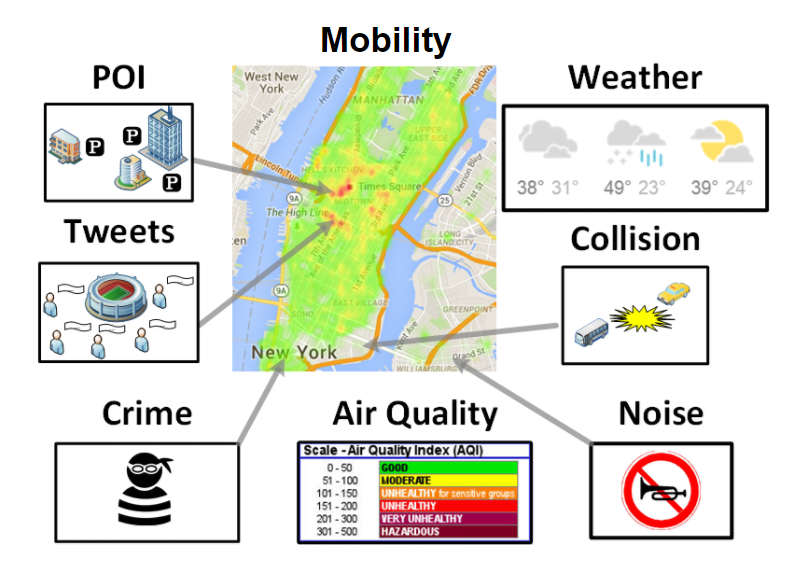
\includegraphics[width=0.8\linewidth]{fig/intro-data-v2.png}
\caption{Various big data collected in urban space.}
\label{fig:intro}
\end{figure}

All those urban data provides amazing opportunities for us to study urban problems and build intelligent urban applications. Among all these data, the urban mobility data is especially interesting because the mobility flow connect a pair of locations. 


\section{Model Mobility-Flow-Incurred Interactions}


In the urban space, the movement of human population connects two disjoint regions, and brings influence from one to the other. My research focuses on modeling the complicated interactions in the urban space with human mobility data.  


In recent years, there are some large datasets of urban taxi made public~\cite{nyctaxi} under the Freedom of information request law.  The taxi dataset contains the time and location of pick-up and drop-off for a trip. By aggregating the taxi data, we are able to get the mobility flow among different regions.
Mobility flow data (e.g., commuting flow, taxi trajectories) are sensitive resources that urban planners can use to address city issues.




Consider the following two examples. These two examples show that it is not sufficient to only consider spatial interaction, and the interactions incurred by mobility flow is equally important.


\textbf{Example 1.} \emph{Policy makers are deciding where to construct a shelter for families that are victims of violence. They understand the value of locating the shelter geographically far from violent neighborhoods. One possible choice is to locate the shelter in a neighborhood that is 10 miles from the violent neighborhoods where vulnerable families previously lived. However, a deeper analysis may reveal that the new neighborhood, though geographically removed from the old neighborhood, may still have strong social flows (connections caused by commutes, family visits) with the old neighborhood. Emerging research suggests that a great deal of crime happens in areas that are socially connected to offenders' neighborhoods. This suggests that shelters may benefit from being located in a neighborhood that is also socially isolated from violence (e.g., with weak communication and commuting interactions with the violent neighborhoods that shelter residents fled from) while socially connected to jobs, services, and resources.}


\textbf{Example 2.} \emph{In order to provide better living environment to crowded city, city planner decide to expand city with a new satellite town. However, people are not willingly to move, if there is not enough incentive. To create opportunity and attract people, some candidates to relocate are big factory, shopping mall, and government offices. The question is which facility should be relocated, so that population pressure in whole  city  is relieved.  Correspondingly, how many new residential building, supermarket, and parks should be built into the new city? People have to go the new city to work. Some of them may move to live in the new city, and the rest may choose to commute everyday.}





\section{Research Problems}
\label{sec:qa}


In this dissertation, we model the city as a spatial network of regions, where each region is one node and there is a link between a pair of nodes. Links measure the interactions between a pair of regions. For example, the spatial link defines the spatial adjacency among regions. There are other types of links as well.  Accounting for these different types of region \textbf{interactions} can improve the a set of urban prediction tasks. I am specifically interested in the mobility flow data because they act as a type of ``hyperlink'' and connect regions that are spatially far away. In order to model the city as a spatial network, we have to answer the following three research questions.

\begin{itemize}
\item How to better understand nodes using links? In an urban prediction task, we usually estimate an unobserved property of a focal region from the observations of similar regions. The challenge lies in an appropriate definition of ``similar regions''. In the literature, spatial similarity is widely used. However, we argue that mobility flow also plays an important role in defining region similarity. For example, the crime rate in a residential neighborhood could be impacted by spatially non-adjacent but flow-connected neighborhoods.
\item How to define appropriate nodes in the spatial network? The administrative boundaries are widely used to define discrete regions. However, there are also a lot of concerns with the predefined boundaries. What if we do not have the boundaries available? What if the current boundary is outdated? Is the predefined boundary suitable for our prediction task?
\item What is the appropriate model for the correlations among various data in our spatial network? We argue that one global model cannot necessarily fit all scenarios. For example, nationwide we may observe that the house price is negatively correlated with house density. However, such observation is not universally true because we can easily find counterexample. For example, the house price in Manhattan island is high regardless of the high house density.
\end{itemize}




\section{Interactions within Networks in the Literature}
\label{sec:ew}



\subsection{Spatial Interaction Model}


Spatial interaction is a broad term encompassing any movement over space that results from a human process \cite{haynes1984gravity,rodrigue2013geography}. It measures the flow between an origin and a destination, given distance and nodal properties on the origin and destination.  There are several classic models to measure the spatial interactions. For example, \textbf{gravity model} \cite{matyas1997proper} uses a similar formulation than Newton's law of gravity to model the interaction between two regions.
\textbf{Spatial autoregressive model} \cite{anselin1980estimation} is another widely used inference model that infer a property in a region with nearby region's information. There are a lot of  applications  based on the spatial interactions, such as international trade \cite{carrere2006revisiting, egger2003proper, martinez2003augmented}, population migration \cite{hanski1994metapopulation, karemera2000gravity, lewer2008gravity}, traffic flow \cite{jung2008gravity, roughan2002experience, khadaroo2008role}, telecommunication flow \cite{krings2009urban, fischer1994artificial, black1995spatial}, crime estimation \cite{anselin2000spatial, kakamu2008spatial, browning2004paradox}, knowledge spillover \cite{lesage2007knowledge, fischer2006geography}, and many more.



Notice that the region interaction in this thesis proposal is different from the traditional \textbf{spatial interaction} study, which assumes the interaction of two regions is reversely correlated with their geographical distance. However, space is a biased sample on human mobility, and should not be the only measure to model human movement. For example, during the weekdays people usually follow a regular home-office commuting pattern. The workplace region might be far from home region, but their connection is strong due to the human movement. As there are more and more mobility data available, we propose to employ the flow data in the interaction model as well.







\subsection{Exploring Mobility Flow}

In recent years, the availability of flow data enables research progress on exploring the role of various flows. New observations are made on the mobility data. For example, there are studies to explain epidemic spread with air travel \cite{huang2013global, tatem2014mapping} and population migration survey \cite{pindolia2013demographics}. Zheng et al. \cite{zheng2011urban} identify the underlying road network problem by detecting anomalous pair of flow. Yuan et al. \cite{yuan2012discovering} discover the function of regions by learning a topic model on the flow matrix and clustering the flow of region pairs into different topic.  Berlingerio et al. \cite{berlingerio2013allaboard} optimizes public transport route by looking at the region origin/destination flow. 



The problem in this proposal is different from the works above in the sense that different approaches are taken. Those works in the literature study the mobility flow by itself. Namely, the literature focuses on observing the properties of the mobility flow by various data mining technique, such as clustering \cite{berlingerio2013allaboard}, topic modeling \cite{yuan2012discovering}, outlier detection \cite{zheng2011urban} etc.  The approach in the literature uses the observed properties of flow to manually explain a phenomenon. This thesis proposal takes a different approach, that explicitly models the statistic dependency between social flow and region properties in an inference problem setting. The approach in this thesis allows us to answer those three research questions raised in Section~\ref{sec:qa}, which the literature methods cannot answer.





\subsection{Interaction Model in Social Networks}


In social network analysis, there is a line of work that focuses on infer an unobserved  nodal feature from neighboring nodes. Examples are infer user home location \cite{Pontes:2012:WKY:2370216.2370419, Li:2012:TSU:2339530.2339692}, user age \cite{6195711}, and more categorical features \cite{Mislove:2010:YYK:1718487.1718519}. Earlier works mainly focus on one type of features, and employ the network structure to make inference. To solve the application problem of user profiling, some techniques are borrowed from community detection \cite{fortunato2010community}, information diffusion \cite{guille2013information}, collaborative filtering \cite{breese1998empirical}, etc. The inferred features are assumed to be similar within a cluster. Therefore, community detection will cluster nodes with unobserved property together with nodes with observed property, and thus we can conduct inference. Another angle is to study how information is propagated through network. Methods under the information diffusion category is explanatory \cite{rodriguez2011uncovering, gomez2010inferring}.


With more data types available, there is one line of works solving the nodal feature inference problem with \textbf{composite social network} \cite{pan2011composite, madan2011pervasive,zhong2012comsoc}. Composite social network is a graph with multiple types of edges. For example in a social network, two users could be connected by following, how many re-tweets, how many messages are exchanged, etc. 


Our work is different from those work in social network literature in a way that we do not use observed edge strength as the interactions. All those paper in literature assumes that if two nodes are connected by a edge with heavy weight, then they are very likely to have strong interactions. This is not necessarily true. Take the crime inference as example. Suppose two communities are connected by heavy traffic flow, and both community are crime free. In this case, we cannot say two regions have strong crime interactions.







\section{Challenges}

There are mainly three challenges to address.

\textbf{Given multiple types of social flow, the interaction is difficult to define}. Given only one type of social flow, there are too many possibilities in constructing interactions.  First, the flow matrix can take various form. For example, we can chose normalize the flow matrix or not. When normalizing the flow matrix, we can chose whether normalize by in-flow or out-flow. Second, there are many nodal properties that could interact with their neighbors, such as various demographics features. Third, different kinds of function can be used to define interactions. Take the product of flow and nodal properties is the most straightforward choice. However, sometimes it also makes sense to further apply distance exponential decay on previous product.  Furthermore, it is possible we have multiple types of social flow (e.g. taxi flow, commuter transit). For one pair of regions, should we build separate interaction over different social flows, or sum over all flows to get one interaction? When we take the sum, should we weight different social flow differently, and how?



\textbf{Identify discrete node from continuous space is challenging}. In the literature, the boundary of regions are usually pre-defined administrative regions, which has two major issues. First, this boundary definition is not consistent in terms of the property of interest. For example, it is very likely a community is formed on the boundary of two administrative regions. Also, the current partition does not evolve over time. In real life, we know there must be some dynamic change of communities. Second, partition continuous space is not trivial. There is a misalignment problem, which refers to the problem that different data are not collected in the same scale. For example, the crime record is at point level, while the demographics is at block level.



\textbf{The interaction is non-stationary over the space}. Most models in existing work are global model, which assumes the statistic interaction does not vary over space. However, some urban data have spatial non-stationary property. Therefore, using global estimates of relationships can present misleading interpretations of local relationships. \\


To address these challenges, I have three : (1) use graph embedding method to incorporate heterogeneous region interaction data; (2) use geographically weighed graphical model to account for the spatial non-stationary property; (3) automatically learn task-specific community area partitions.



\section{Organization}


The rest of my dissertation is organized as shown in Figure~\ref{fig:org}. In Chapter~\ref{ch:preliminary} I give a preliminary study to verify the idea that using mobility flow as hyper-links to better model region similarity. We use crime inference as an example, in which we use an enhanced spatial autoregressive model to predict crime count of a community using its neighbors.

To address the aforementioned three challenges, I have correspondingly three major components in my dissertation. I propose an embedding method to incorporate all kinds of region interactions in Chapter~\ref{ch:embedding}. Next, I study the task-specific region partition problem in Chapter~\ref{ch:partition} to tackle the spatial continuity. In Chapter \ref{ch:non-stationary}, we first identify the spatial variations in mined relations. We further employ a geographically weighted regression model to solve the problem. Finally, I conclude in Chapter~\ref{ch:conclusion} with a discussion of potential future topics.


\begin{figure}[h]
\centering
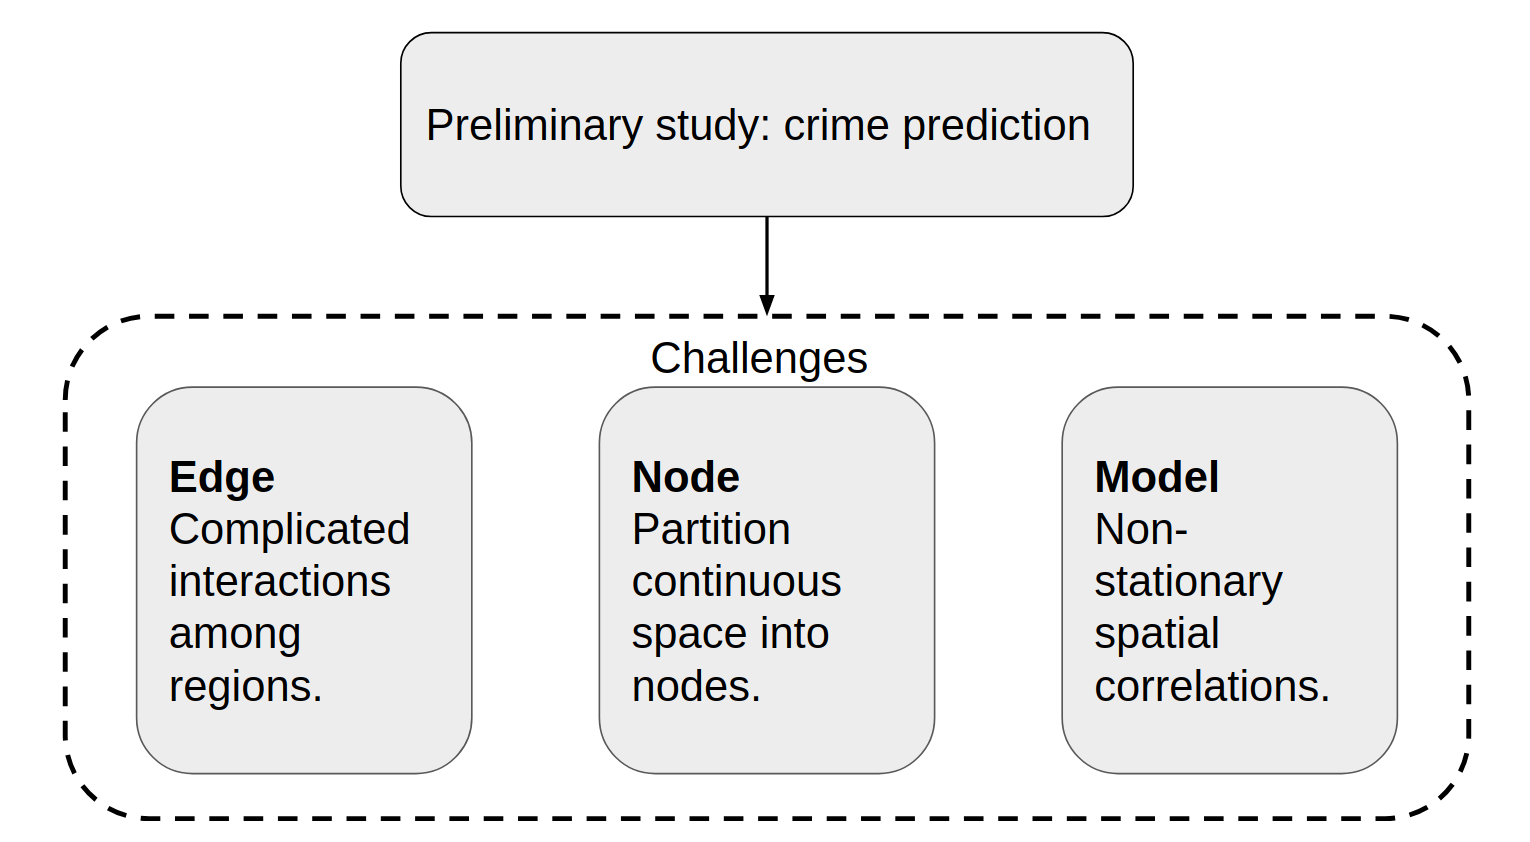
\includegraphics[width=\linewidth]{fig/organization.png}
\caption{Organization of this dissertation.}
\label{fig:org}
\end{figure}



\chapter{Understand Nodes Using Links}
\label{ch:preliminary}



In this chapter we address the first proposed research question. Namely, we use the observations in other regions and other types of data to estimate one unobserved property in focal region. We call this problem \textbf{inference problem}. At the very beginning, we give a generalized inference problem definition. Following the general definition, we look at one example of crime inference.


\section{General Problem Definition}

In this section, we give a generalized definition of the inference problem. Suppose we have a set of regions $r_1, r_2, \cdots, r_n$, and we are interested in one property $y_i$ for region $r_i$. In addition to $\vec{y}$, we also have other properties $\vec{x}_i$ observed on region $r_i$, and the set of all auxiliary properties are denoted as $X$. It is noteworthy that both $\vec{y}$ and $X$ are nodal properties. The spatial adjacency among all regions are known as $W^0$, where $W^0$ is spatial adjacency matrix. The hyperlink mobility flow is also observed as $W^k$ for type $k = \{1, 2, \cdots\}$. The entry $w_{ij}^k$ in $W^k$ refers to the quantity flow from $r_i$ to $r_j$ of type $k$.


The inference problem is that for a given region $r_t$, whose $y_t$ is unobserved, we try to use $\{y_i \} \backslash y_t$ together with $X$ and $W^k, k \in \{0, 1,2, \}$ to estimate $y_t$. Mathematically, we have
\begin{equation}
\hat{y_t} = f( \{y_i\} \backslash y_t, X, W^k),
\end{equation}
where $f$ is the estimation model of any choice.




In the next section, we will use the crime inference as  an example to show how this inference problem is solved in the literature, and how do we enhance the existing model.



\section{Crime Inference as One Example}


\begin{figure}[t]
\centering
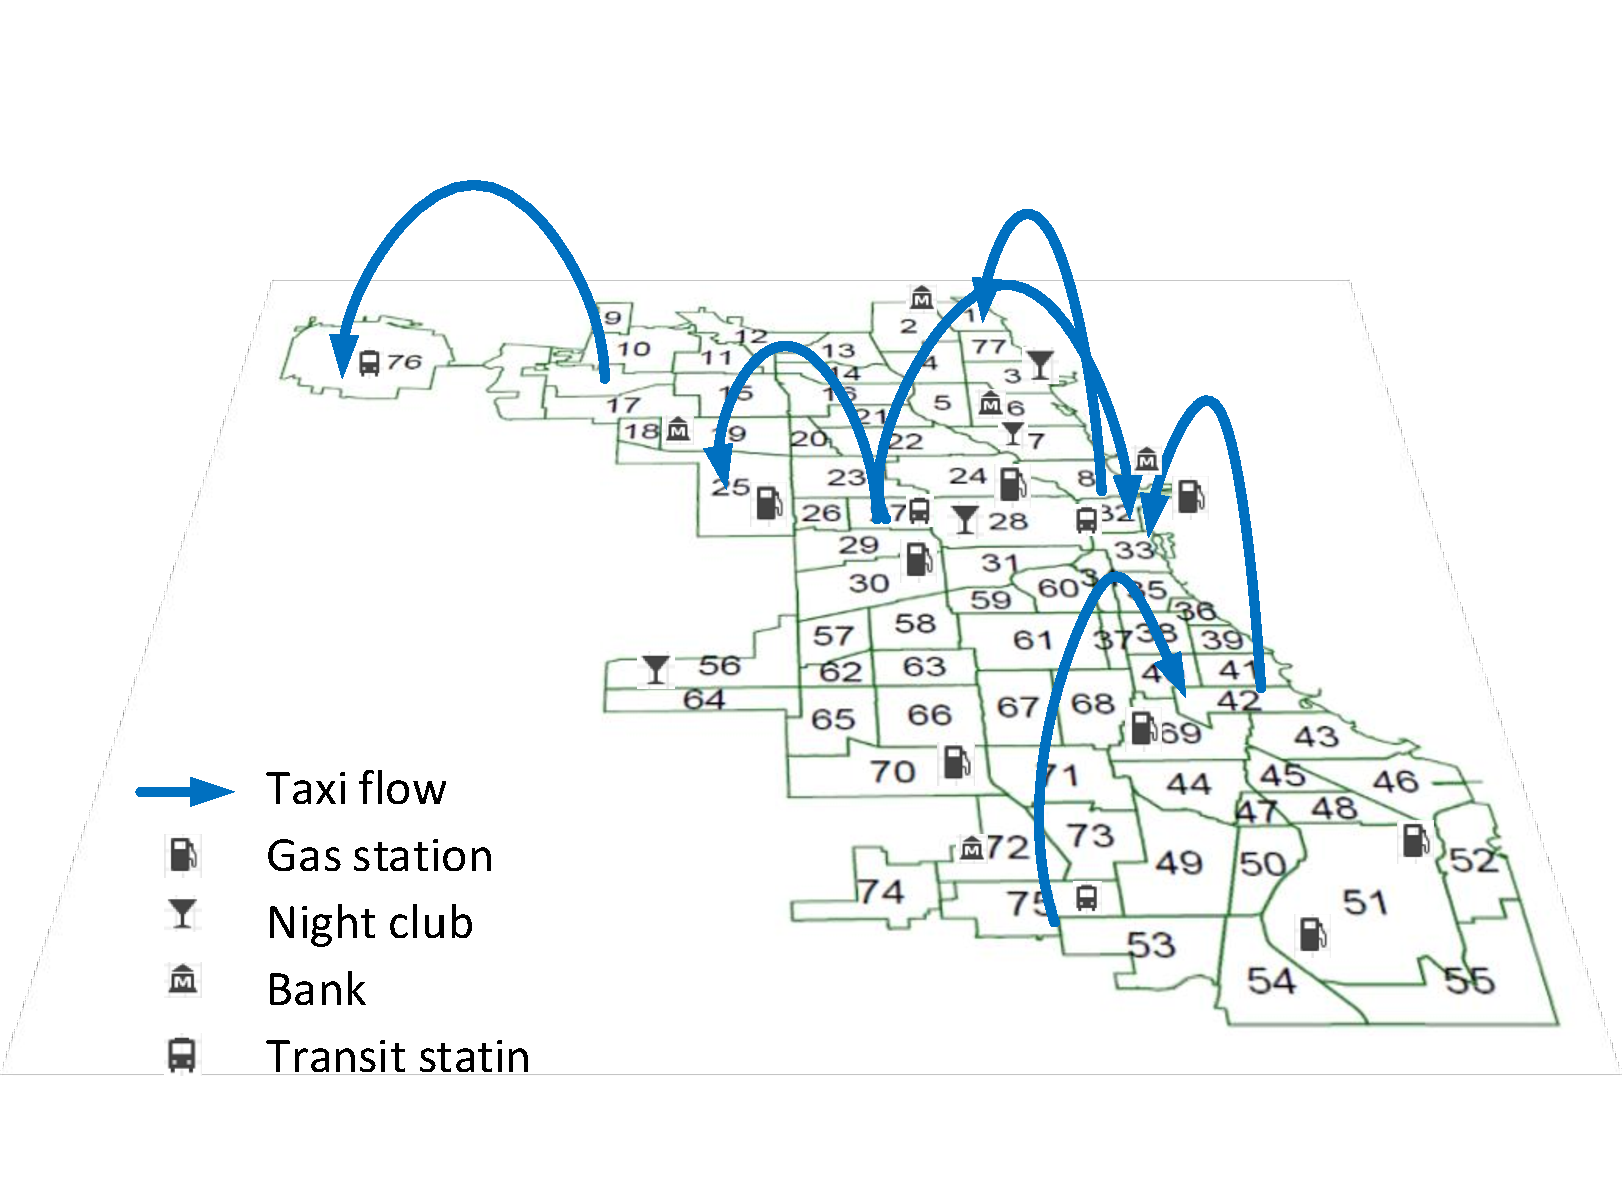
\includegraphics[width=0.8\textwidth]{fig/demo.pdf}
\caption{An illustration of various types of features we used in Chicago. The POI distribution across community areas reflects profiles of the region functionality. The taxi flow connects nonadjacent regions and act as a ``hyperlink''.}
\label{fig:demo}
\end{figure}



In Figure~\ref{fig:demo}, we show that taxi flow as a newer type of big data could provide us new insights to understand some traditional socioeconomic urban problems.  A huge amount of taxi flow data reflect how people commute in the city. In previous studies, when using geographical influence~\cite{Ans02}, people assume that a community is affected by the spatially nearby communities. However, communities are not only affected by spatially-close communities. Even if two communities are distant in geographical space, they could have a strong correlation if there are many people frequently travel between these two communities~\cite{GGM14}. We hypothesize that taxi flows may be considered as ``hyperlinks'' in the city that connect the locations and we use such data to estimate crime rates. Our experiments show very promising results --  adding taxi flow data on top of all other features can further decrease the error by 5\%.


\subsection{Related Work}


In the criminology literature researchers have studied the relationship between crime and various features. Examples are historical crime records~\cite{MSBS+12,WRWS13}, education~\cite{Ehrl75}, ethnicity~\cite{Brai89}, income level~\cite{Patt91}, unemployment~\cite{Free99}, and spatial proximity~\cite{Ans02}. 
In data mining field, newer type of data are used in the study. For example, there are works using twitter to predict crime \cite{WGB12,Gerb14}, and works using cellphone data \cite{TQC14,Bogo14} to evaluate crime and social theories at scale. 


Overall, the existing work on crime prediction can be categorized into three paradigms.



\textbf{Time-centric paradigm}. This line of work focuses on the temporal dimension of crime incidents. For example, in a study \cite{MSBS+12}, the authors propose to use a self-exciting point process to model the crime and gain insights into the temporal trends in the rate of burglary. In another study \cite{Ratc06}, the authors investigate the temporal constraints on crime, and propose an offender travel and opportunity model. This paper validates the claim that a proportion of offending is driven by the availability of opportunities presented in the offender's routine lives. 


\textbf{Place-centric paradigm}. Most existing work adopt a place-centric paradigm, where the research question is to predict the location of  crime incidents.  The predicated crime location is usually refereed by the term \emph{hotspot}, which has various geographical size.  There are plenty of works on exploration of the crime hotspots. For example, in a study \cite{TEP11} the authors  use criminal offense records to identify spatio-temporal patterns at multiple scales. They employ various quantitative tools from mathematics and physics and identify significant correlation in both space and time in the crime behavioral data.  Short \emph{et al.} \cite{SDPT+08} use a simple model to study the dynamics of crime hotspots and identify stable hotspots, where criminals are modeled as random walkers.  Bogomolov \emph{et al.} \cite{Bogo14} use human behavioral data derived from mobile network and demographic sources, together with open crime data to predict crime hotspots. They compare various classifiers and find random forest has the best prediction performance. The paper \cite{WGB12} bases on automatic semantic analysis to understand natural language Twitter posts, from which the crime incidents are reported. Some other work \cite{CTU08,ECCW05} employ the kernel density estimation (KDE) to identify and analyze crime hot spots. Those works form another form of crime prediction, which relies on the retrospective crime data to identify areas of high concentrations of crime. In  \cite{NaYa14}, the authors extend the crime cluster analysis with a temporal dimension. They employ the space-time variants of KDE to simultaneously visualize geographical extent and duration of crime clusters. 




\textbf{Population-centric paradigm}. In the last paradigm, research focuses on the criminal profiling at individual level and community level. At the individual level, \cite{WRWS13} aim to automatically  identify crimes committed by same individual from the historical crime database. The proposed system called \emph{Series Finder}, is designed to find and classify modus operandi (M.O.)  of criminals.  At the community level, Buczak \emph{et al.} \cite{BuGi10} use fuzzy association rule mining to find crime pattern. The rules they found are consistently held across all regions. The paper constructs association rules from population demographics in community.  In another paper \cite{TQC14}, the authors use computation method to validate various social theories at a large scale.  The data they used is mobile phone data in London, from which they mine the  people dynamics as features to correlate with crime.  


Our problem is different from the first two categories of work, mainly because our innovation mostly lies in using newer type of data to enhance the commonly used traditional counterpart. More specifically, we use POI to enhance the demographics information, and use taxi flow as hyper link to enhance the geographical proximity correlation. Although our problem does not consider the temporal dimension of crime in depth, it could be a promising supplement to better profile crime. Our problem dose not predict the location of any particular crime incident. Therefore the methods proposed in place-centric method are not applicable in our problem. However, the features we proposed may be incorporated in those crime prediction model. 
Our problem falls into the third paradigm,  because we are trying to profile the crime rate for Chicago community areas. In our problem, the community areas are well-defined and stable geographical regions. The newly proposed POI feature and taxi hyper link provide a unique perspective in profiling the crime rate across community areas.




\subsection{Data Description and Feature Extraction}

The crime dataset in Chicago has detailed information about the time and location (i.e., latitude and longitude) of crime and the types of crime. In our problem, when we use term crime count, we often refer to crime count in a  region (i.e., community area) in a year. The \emph{community area} is used as our geographical unit of study, since it is well-defined,  historically recognized and stable over time~\cite{wiki-ca}. In total, there are 77 community areas in Chicago.  Crime rate is the crime count normalized by the population in a region. We use vector $\vec{y} = [y_1, y_2, \ldots, y_n]$ to denote the crime rate in region $i$.


The crime data of Chicago are obtained from City of Chicago data portal~\cite{crime-data}. Chicago is the city with most complete crime data that are made public online. The crime dataset contains the incident date, location (strict name and GPS coordinates), and primary type from year 2001 to 2015. In total there are $5,856,414$ recorded crime incidents over 15 years, which is an average $390,417$ crimes incidents per year. We visualize the crime normalized by population in Figure~\ref{fig:crime-ca}, from which we can see that the downtown area has the highest crime rate.

\begin{figure}[t]
\centering
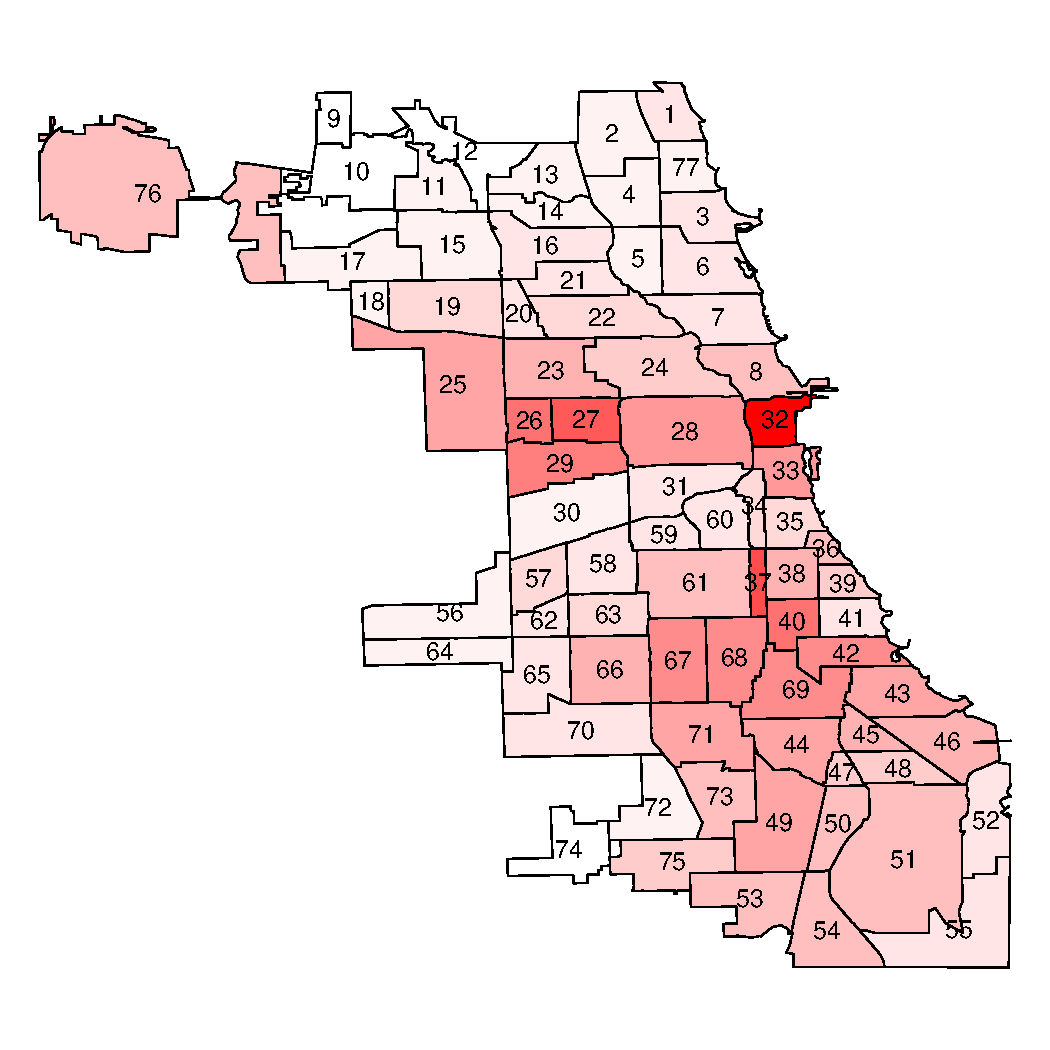
\includegraphics[width=0.7\textwidth]{fig/crime-ca.pdf}
\caption{Crime rate of Chicago by community areas. The community area \#32 is Chicago downtown, which has the highest crime rate.}
\label{fig:crime-ca}
\end{figure}


In this example we study the crime rate inference problem. More specifically, we estimate the crime rate of some regions given the information of all the other regions. Without loss of generality, we assume there is one community area $t$ with crime rate $y_t$ missing, and we use the crime rate of all the other regions $\{y_i \} \backslash y_t$ to infer this missing value. Our problem is mathematically formalized as follows
\begin{equation}
\hat{y_t} = f( \{y_i\} \backslash y_t, X),
\end{equation}
where  $X$ refers to observed extra information of  all those community areas.


\smallskip
We consider two  types of features $X$ for inference:
\begin{itemize}
\item Nodal feature. Nodal features describe the characteristics of the focal region. Such features include demographic information and Point-of-Interest (POI) distribution. Demographics are frequently used in literature, but POI is a newer type of big data, which we find significantly improve the crime inference accuracy.
\item Edge feature: (1) Geographical influence. Geographical influence considers the crime rate of the nearby locations.  This feature has been extensively used in
literature as well. To estimate the focal region, the
crime rate of nearby regions are weighted according
to spatial distances. (2) Hyperlink by taxi flow. Locations are connected through the frequent trips made by humans, which can be considered as the hyperlinks in space. This type of feature has never been studied in literature. We propose to use taxi trips to construct the social flow. Our hypothesis is that similarity in the crime rate of two regions should correlate with the social flow strength between these two regions. 
\end{itemize}



Below we will describe the datasets used to construct features and the characteristics of these features.

\begin{figure*}[t]
\centering
\subfigure[Total population]{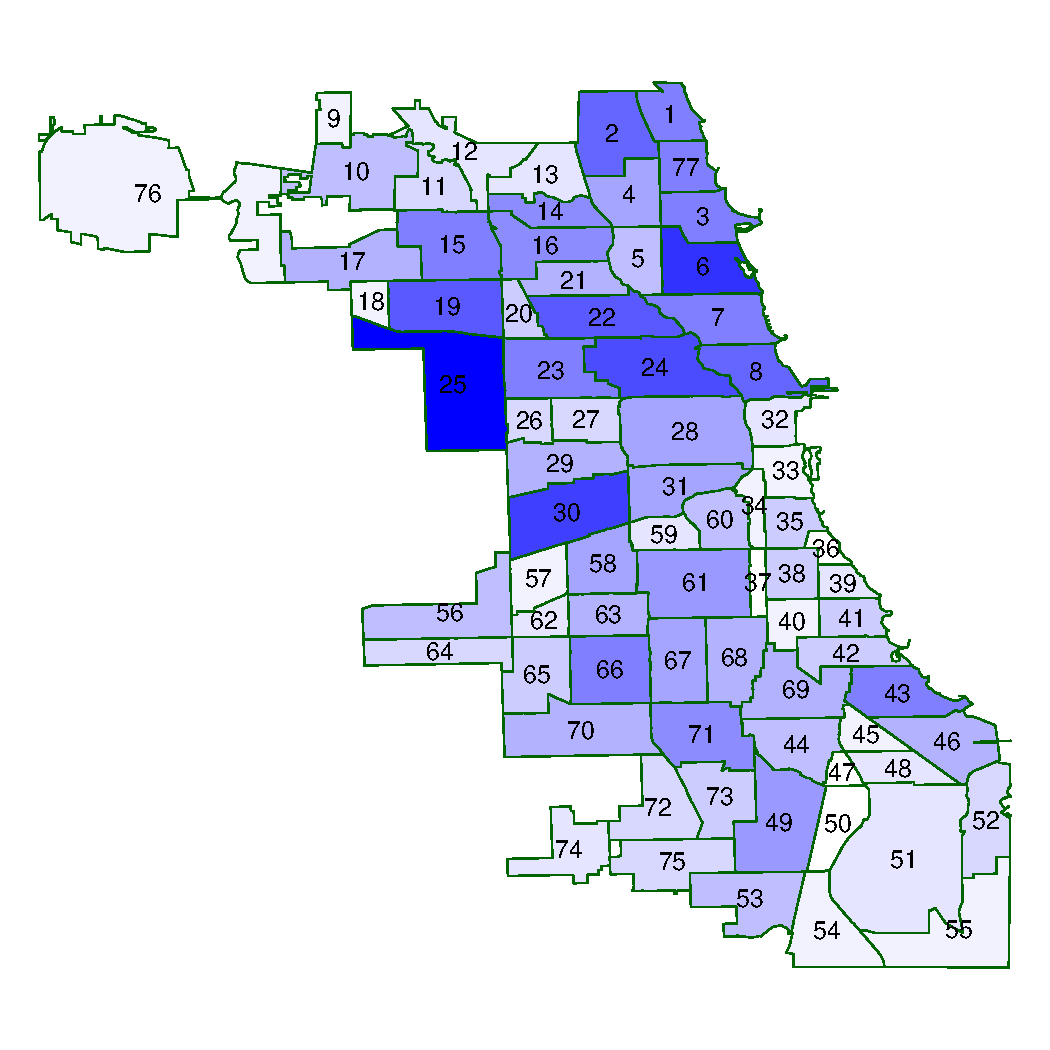
\includegraphics[width=0.45\textwidth]{fig/demo-f1.pdf}}
\subfigure[Poverty index]{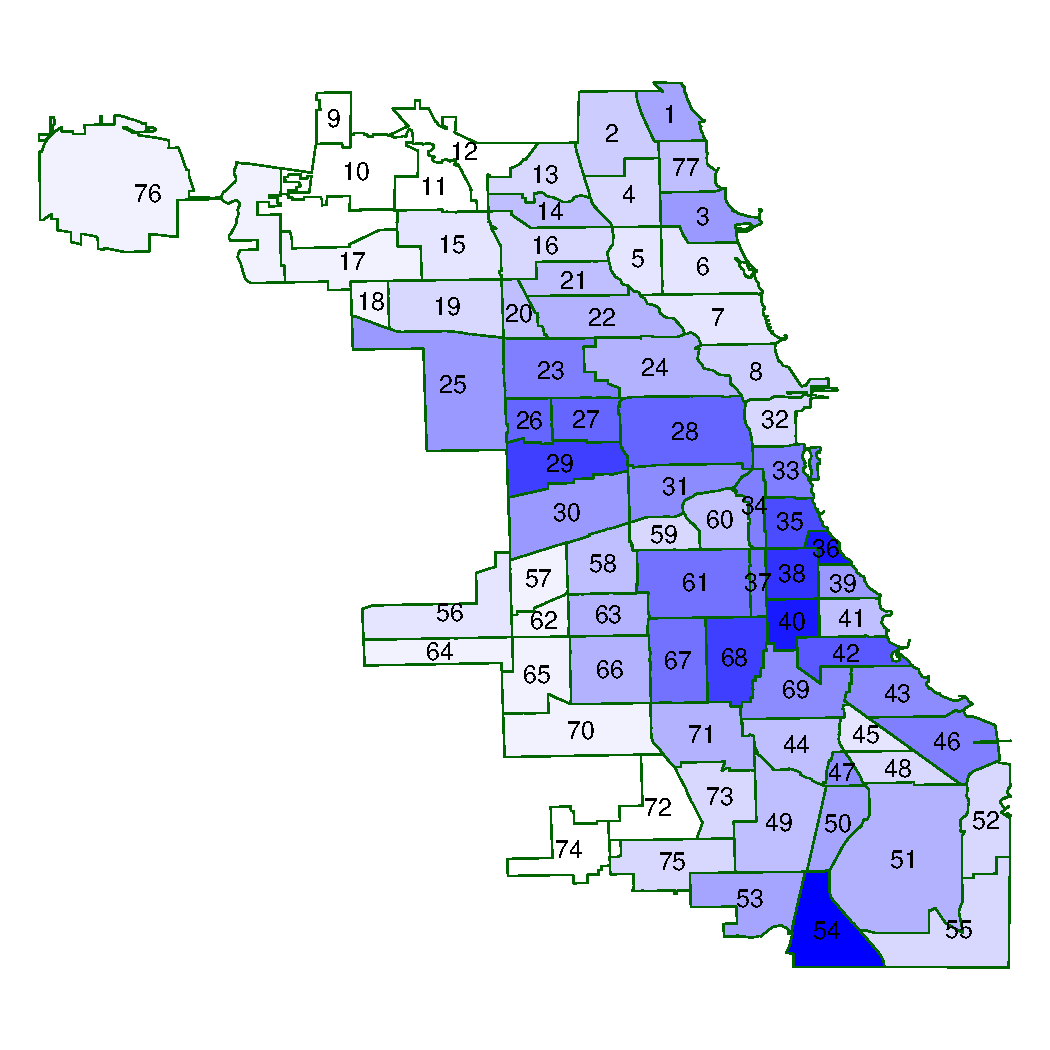
\includegraphics[width=0.45\textwidth]{fig/demo-f3.pdf}}
\subfigure[Disadvantage index]{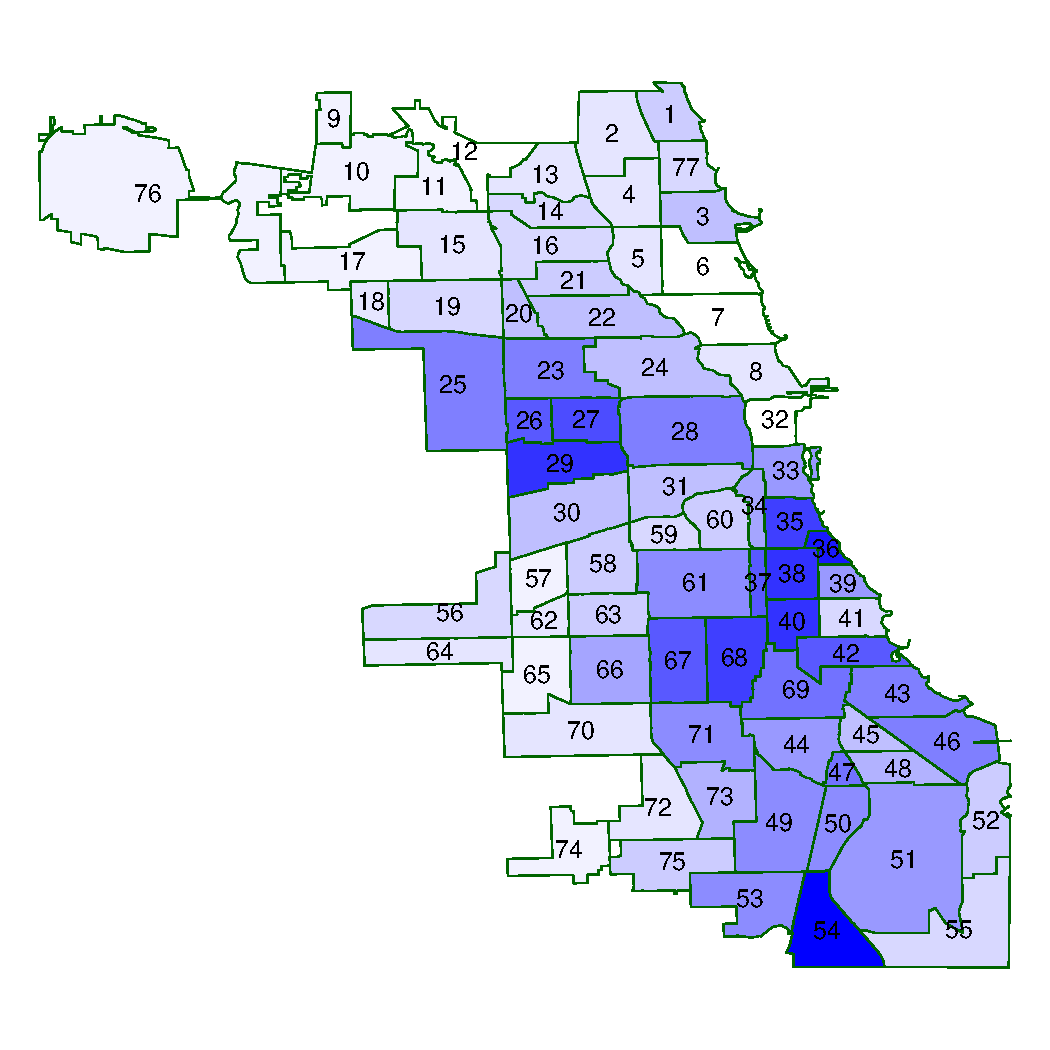
\includegraphics[width=0.45\textwidth]{fig/demo-f4.pdf}}
\subfigure[Ethnic diversity]{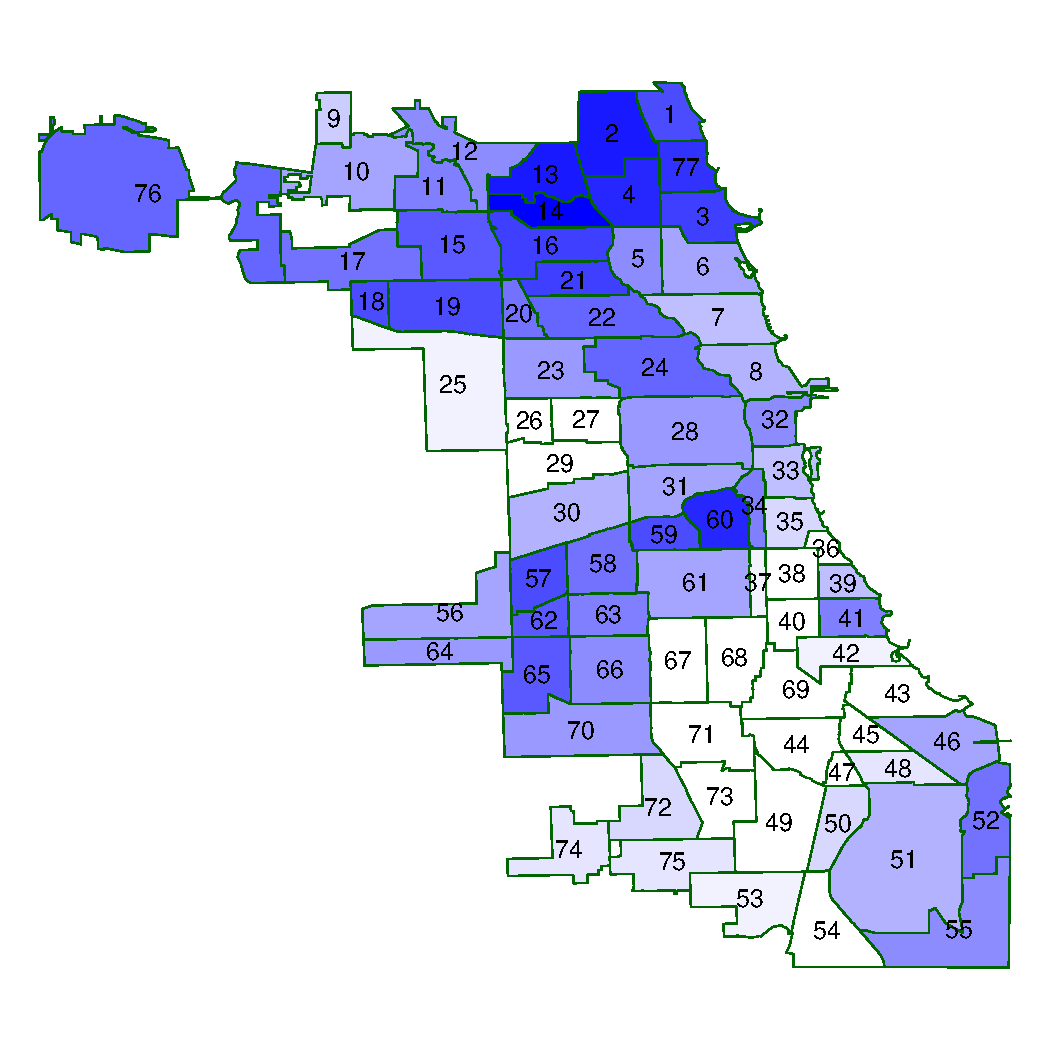
\includegraphics[width=0.45\textwidth]{fig/demo-f6.pdf}}
\caption{(a)-(d) Demographics in Chicago by community areas. Darker colors indicate higher values.}
\label{fig:demo-f}
\end{figure*}





\textbf{Nodal Feature: Demographics}

Socioeconomic and demographic features of neighborhoods have been
widely used to predict crime~\cite{Bogo14, HsPu93, WoMe12, SaHi07}. Previous studies have shown that crime rate correlates with certain demographics. For example, \cite{Jac61, GrSa09} suggests that population diversity leads to less crime in certain neighborhoods. 
In our study, we include demographic information from the US Census Bureau's Decennial Census of 2010~\cite{census-data} and American Community Survey's five-year average estimates
between 2007 and 2011. We use year 2010 data because we are evaluating crime rates in 2010-2013. The demographics include the following features:

\textsf{total population, population density, poverty, disadvantage index, residential stability, ethnic diversity, race distribution}.


The poverty index measures the proportion of community area residents
with income below the poverty level. The disadvantage index is
a composite scale based on prior work \cite{SRE97}, a function of 
poverty, unemployment rate, proportions of families with public
assistance income, and proportion of female headed households. 
 The residential stability measures home ownership and proportion of
residents who lived in the neighborhood for more than one year. Racial
and ethnic diversity is an index of heterogeneity~\cite{GrSa09} based on six
population groups, including: Hispanics, non-Hispanic Blacks, Whites,
Asians, Pacific Islanders and others.


Figure~\ref{fig:demo-f} visualizes the crime rate and demographics features in Chicago by community areas. Comparing with Figure~\ref{fig:crime-ca}, it is clear that the crime rate and poverty index and disadvantage index are consistent,  the ethnic diversity shows an inverse correlation, and the total population has little correlation with crime.



Table~\ref{tb:demo} shows the Pearson correlation coefficient between various demographics features and the crime rate at community area level. The corresponding p-value is also calculated and shown in the table to indicate the significance of the correlation coefficient.  There  are in total $77$  community areas in Chicago. Table~\ref{tb:demo} shows such correlation with several most correlated features. We can see that the poverty index and disadvantage index positively and strongly correlate with crime, while the ethnic diversity negatively correlates with crime. Other features such as total population, population density, and residential stability  have weaker correlations. One counter-intuitive observation is that the total population has a weak and negative correlation with crime. The reason is that we use crime rate in each community area, which is already normalized by the population, and therefore the total population and population density have less impact. 


\begin{table}[h]
\centering
\caption{Pearson correlation between demographic features  and crime rate (\textbf{*} indicates significant correlations with p-value less than $5\%$). }
\begin{tabular}{|c||c|c|}
\hline
Feature & Correlation & p-value \\ \hline \hline
Total Population & -0.1269 &  0.2716 \\ \hline
Population Density & -0.1972  & 0.0855 \\ \hline
Poverty Index & \textbf{0.5573*} & 1.403e-07 \\ \hline
Disadvantage Index & \textbf{0.5959*} & 1.082e-08 \\ \hline
Residential Stability  & -0.0453 &  0.6965 \\ \hline
Ethnic Diversity & \textbf{-0.5545*} &  1.678e-07 \\ \hline
Percentage of Black & \textbf{0.6696*} &  2.779e-11 \\ \hline
Percentage of Hispanic  & \textbf{-0.3820*} &  0.0006 \\ \hline
\end{tabular}
\label{tb:demo}

\end{table}







\textbf{Nodal Feature: Point-of-Interest (POI)}

While demographics are traditional census data, POI is a type of  modern data that provide fine-grained information about locations. We collect POI from FourSquare~\cite{poi-data}. POI data from FourSquare provide the venue information including venue name, category, number of check-ins, and number of unique visitors. We mainly use the major category information because categories can characterize the neighborhood functions. There are 10 major categories defined by FourSquare:

\textsf{food, residence, travel, arts \& entertainment, outdoors \& recreation, college \& education, nightlife, professional, shops, and event.}


\begin{figure}[tb]
\centering
\subfigure[Nightlife]{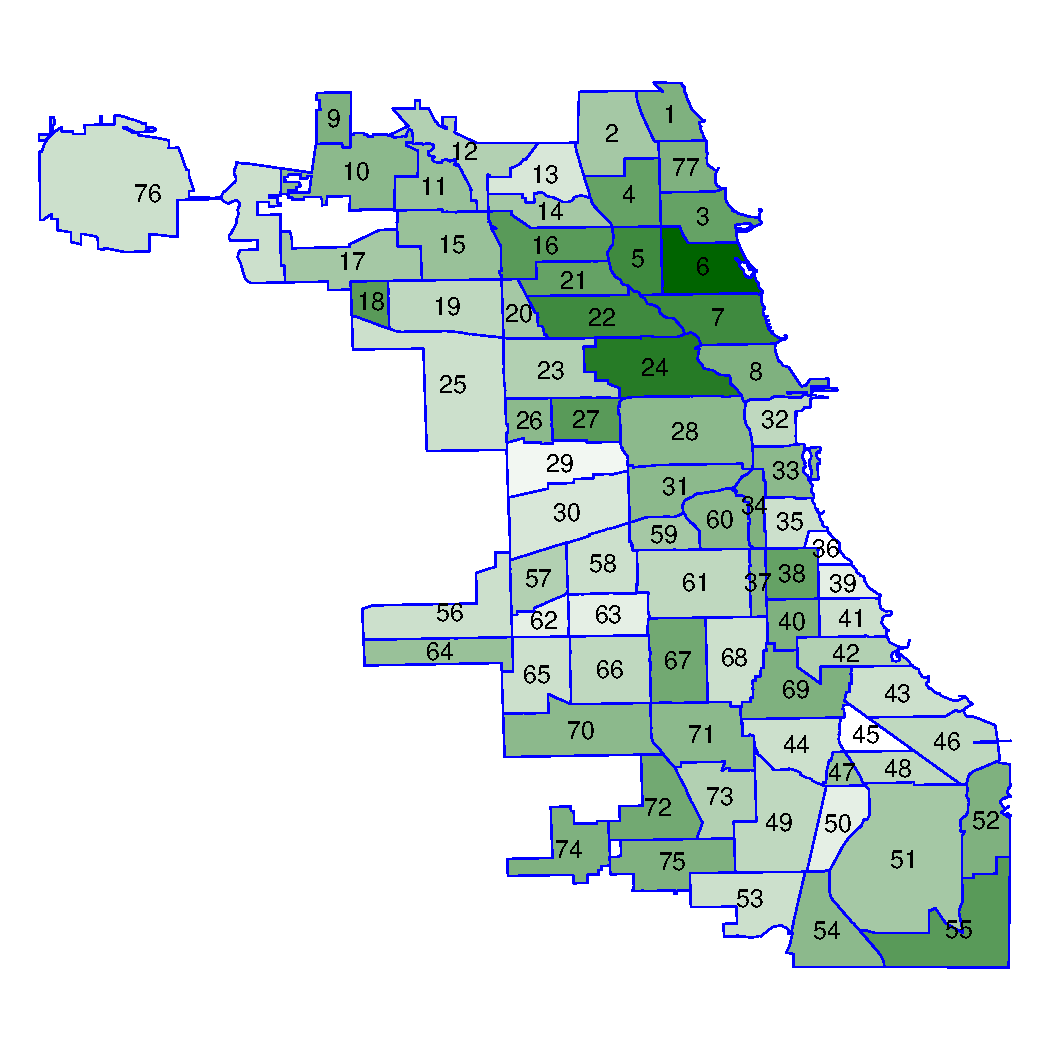
\includegraphics[width=0.45\textwidth]{fig/poi-dist7.pdf}}
\subfigure[Professional]{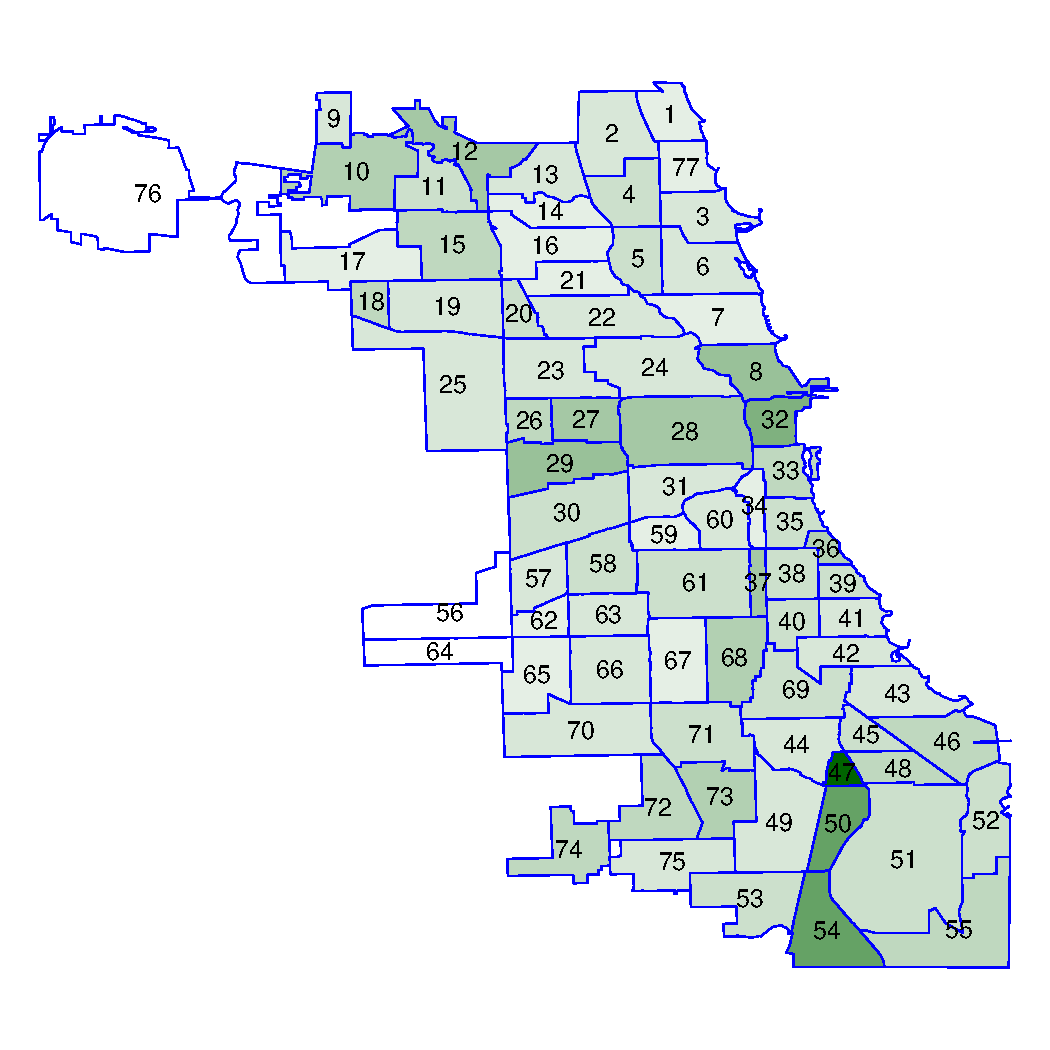
\includegraphics[width=0.45\textwidth]{fig/poi-dist8.pdf}}
\caption{Plot the  POI ratio per neighborhood. The saturation of color is proportional to the ratio value. The ``professional'' category distribution is more consistent with the crime distribution, and therefore it is the most correlated with crime. Meanwhile, the ``nightlife'' category is not positively correlated with Chicago crime.}
\label{fig:poi-coef}
\end{figure}

In total, we have crawled $112,000$  POIs from FourSquare for Chicago. Most of these POIs are in downtown area of Chicago. We normalize the POIs count per category by the total POI count in a neighborhood and plot two selected category, i.e. nightlife and professional, in Figure~\ref{fig:poi-coef}.  The darker colored neighborhoods in Figure~\ref{fig:poi-coef} are the ones with a higher portion of residence POIs.



\begin{table}[h]
\centering
\caption{Pearson correlation between POI category and crime rate (\textbf{*} indicates significant correlations with p-value less than $5\%$).}

\label{tb:poi-corr}
\begin{tabular}{|c ||c|c|}
\hline
POI category & Correlation & p-value \\ \hline \hline
Food & -0.1543 &  0.1803 \\ \hline
Residence &  -0.0610 &  0.5984 \\ \hline
Travel & -0.0017 &  0.9883 \\ \hline
Arts \& Entertainment & -0.0049 &  0.9661 \\ \hline
Outdoors \& Recreation &  0.0668 &  0.5637 \\ \hline
College \& Education & -0.0078 &  0.9473 \\ \hline
Nightlife &  -0.1553 &  0.1775 \\ \hline
Professional & \textbf{0.3221*} &  0.0043 \\ \hline
Shops & -0.1676 &  0.1450 \\ \hline
Event & 0.2196 &  0.0549  \\ \hline
\end{tabular}
\end{table}



In Table~\ref{tb:poi-corr} we show the Pearson correlation between POI category and crime rate. The category ``professional''  is most significantly correlated with the crime rate. Under the professional POI category, there are some venues with a large population concentration, such as transportation center, convention center, community center, and co-working space. In those venues, the  population volume is high and residential stability is low, therefore the professional POI counts positively correlates with crime rate.  One counter-intuitive observation is that ``nightlife'' category is not positively correlated with crime ($-0.1553$). This can be explained through Figure~\ref{fig:poi-coef}(a). The majority of nightlife venues in Chicago locate in northern area, while most crime incidents occur in downtown area.








\textbf{Edge: Geographical Influence}

Together with the US census demographics data, we also collected the boundary shape files of Chicago, which are used to calculate the geographical influence feature.

Previous studies have also shown that the crime rate at one location is highly correlated with nearby locations~\cite{GSGL01, Bur88}. Such geographical influence is also frequently used in the literature~\cite{ACC00, MoSa97}, which is calculated as:
\begin{equation}
\vec{F^g} = W^g \cdot \vec{Y},
\label{eq:spatial}
\end{equation}
where $W^g$ is the spatial weight matrix. If region $i$ and $j$ are not geospatially adjacent, $w_{ij}^g = 0$; otherwise, $w_{ij}^g \propto distance(i,j)^{-1}$.

\begin{figure}[t]
\centering
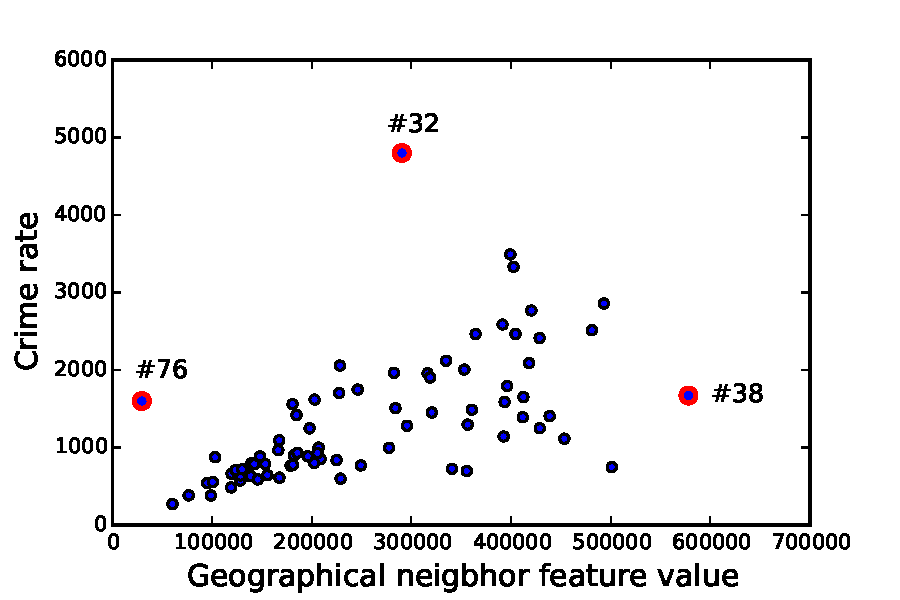
\includegraphics[width=0.8\textwidth]{fig/spatial-crime-rate.pdf}
\caption{The geographical influence feature correlation with crime. In the plot we marked out three outliers and their corresponding community area ID.}
\label{fig:spatial}
\end{figure}

In Figure~\ref{fig:spatial},  we plot crime rate with respect to geographical influence calculated in Eq.~\ref{eq:spatial}. We observe an obvious positive correlation, which means if nearby neighborhoods have a high crime rate, the focal neighborhood is more likely to have a high crime rate. We also do observe a few outliers in Figure~\ref{fig:spatial}. These neighborhoods show different crime rate in their nearby neighborhoods compared to their own. For example, as we can also see in Figure~\ref{fig:crime-ca}, community area \#38 locates in an area where the the neighbors have high crime rates but its crime rate is relatively low; in contrast, neighborhood \#32 has a high crime rate even though its neighbors have relatively low crime. The community area \#76 home of the O'Hare International Airport is far from most of other community areas, however its own crime rate is relative high.





\textbf{Edge: Hyperlinks by Taxi Flow}

In our Chicago taxi dataset, there are $1,048,576$ taxi trips in total during the October to December in 2013. For each trip the following information are available: pickup/dropoff time, pickup/dropoff location, operation time, and total amount paid. We requested the taxi trip records from Chicago taxi commission pursuant of the Freedom of Information Law.  Figure~\ref{fig:taxi-flow} shows a visualization of the major flows at community level.

\begin{figure}[htb]
\centering
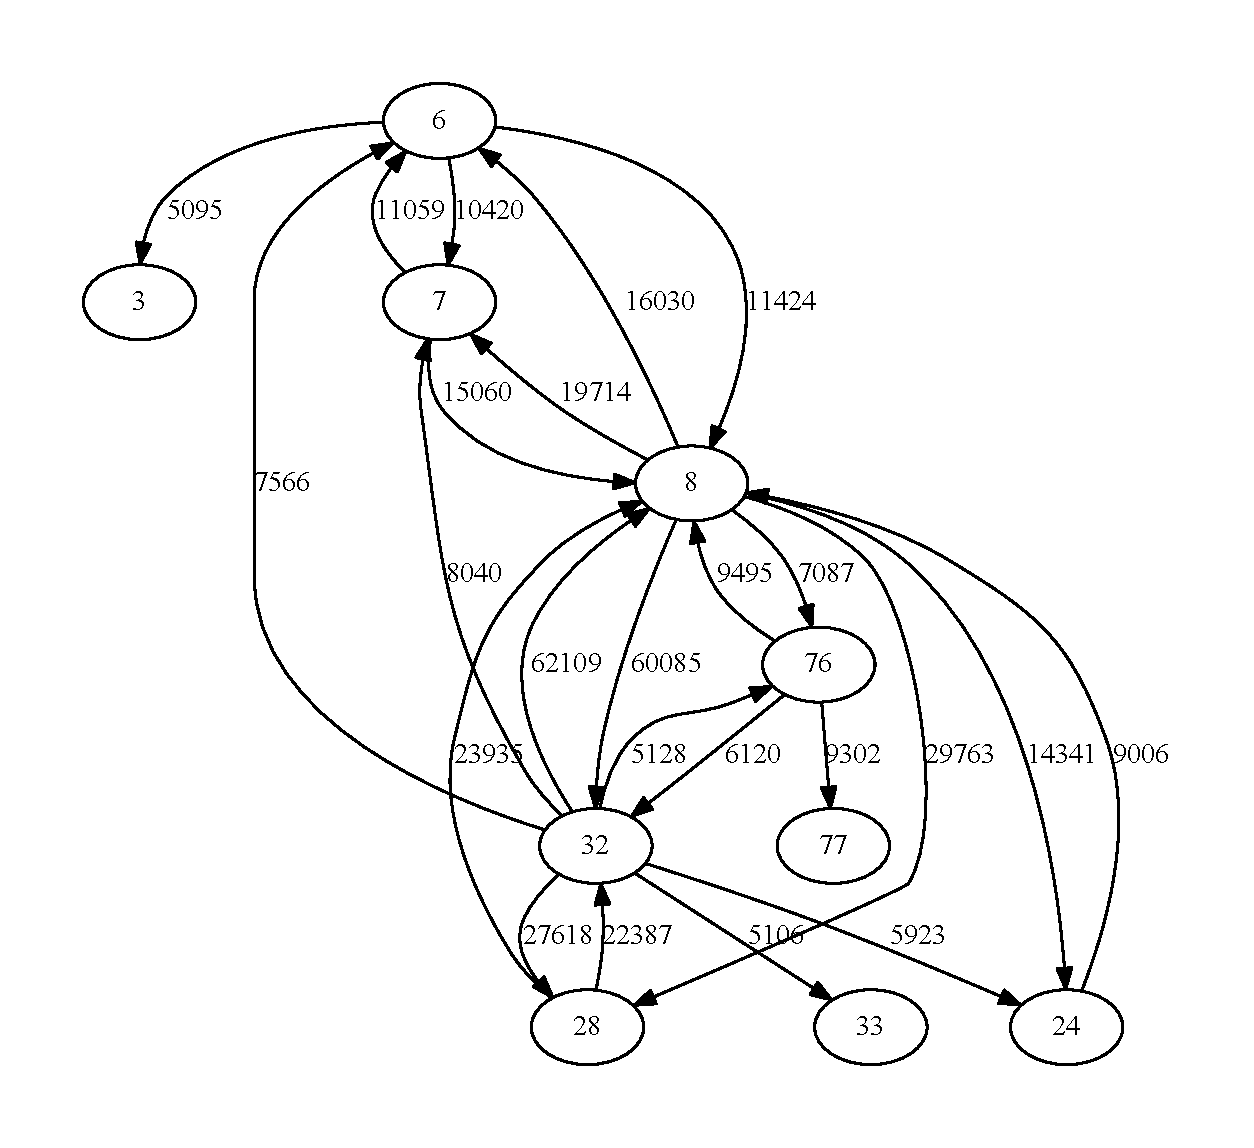
\includegraphics[width=0.8\textwidth]{fig/taxiflow.pdf}
\caption{Major taxi flows between neighborhoods. We set a threshold ($> 5,000$) on the flow and only plot the high volume flow. The label on the node is the ID of the corresponding community areas. We can see that there are several hub community areas, such as \#6, \#8, \#32, which are all in the downtown areas. The label on the edge shows how many taxi trips are commuting through the two community areas for three months in 2013.}
\label{fig:taxi-flow}
\end{figure}


One of our hypothesis is that the social interaction among two community areas propagates crime from one region to another.
The Chicago taxi data captures the social interactions among various community areas. To calculate this first, we first map all taxi trips to community areas to get the taxi flow $w_{ij}\ \forall i,j \in \{1, 2, \cdots n\}$. Then the taxi flow lag is constructed by the product of social flow and the crime rate of neighboring regions as follows
\begin{equation}
\vec{F^t} = W^t \cdot \vec{Y}.
\label{eq:taxi}
\end{equation}
The taxi flow $W^t$ is a matrix with entry $w_{ij}$ denoting the taxi flow from $i$ to $j$. Note that $\forall i$, $w^s_{ii} = 0$ in matrix $W^t$, because we have to exclude the crime in focal area from its own predictor. The semantic of this taxi flow feature is how many crime in the focal area is contributed by its neighboring areas through social interaction.

The correlation between taxi flow and crime rate is shown in Figure~\ref{fig:taxi-corr}. From the scatter plot, we can see that overall the crime rate is positively correlate with the taxi flow. There are two  outliers clearly shown in Figure~\ref{fig:taxi-corr}. The community area \#32 is the downtown Loop, which has the highest crime rate and is hard to predict by taxi flow. Another anomalous community area \#47 has relatively low crime rate by itself. However, this area has a lot of in flows from high-crime communities. 




\begin{figure}[ht]
\centering
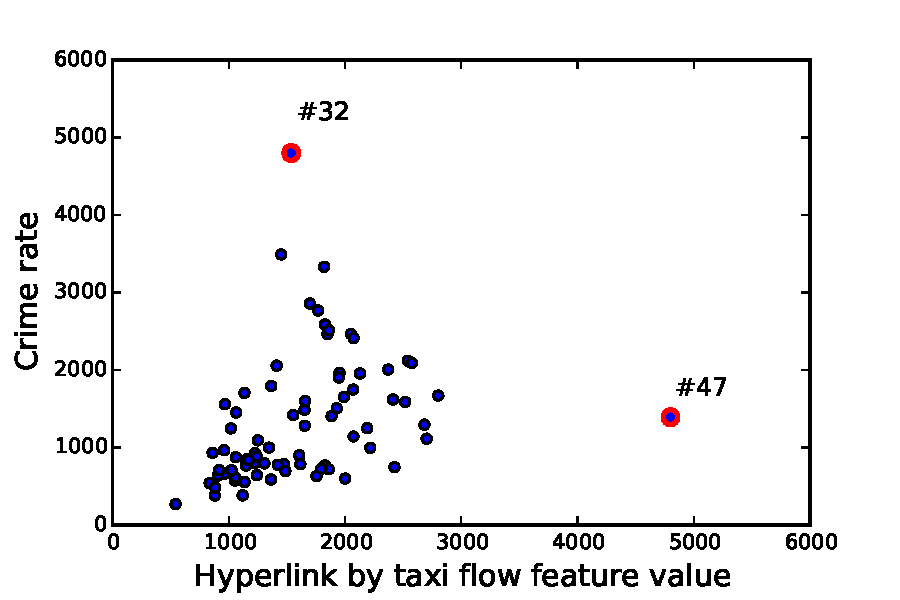
\includegraphics[width=0.8\textwidth]{fig/taxi-flow-percent.pdf}
\caption{Correlation between taxi flow and crime rate. In the plot, we marked out three outliers and their corresponding community area ID.}
\label{fig:taxi-corr}
\end{figure}






\subsection{Spatial Autoregressive Inference Model}



\textbf{Linear Regression}

The most straightforward prediction is linear regression model. This model assumes the error terms follow a Gaussian distribution $\epsilon \sim \mathcal{N}(0, \sigma^2)$. As a result the parameter distribution also follows a Gaussian distribution. This assumption makes the model less generative, since in real applications, there is no way to ensure the dependent variable has a Gaussian error term. 


Equation~\ref{eq:lrm} gives the linear regression formulation of our problem.
\begin{equation}
\label{eq:lrm}
\vec{y} = \vec{\alpha}^T \vec{x} + \beta^f W^f \vec{y} + \beta^g W^g \vec{y} + \vec{\epsilon},
\end{equation}
where $\vec{x}$ represents the nodal features including demographics and POI distribution, $W^f$ is the flow matrix of taxi flow, and $W^g$ is the spatial matrix representing the geographical adjacency. On the right-hand side, $\epsilon$ is the only stochastic variables, and all other terms are fixed observation values. Therefore, we incorporate all the fixed observations into one term $X$, and we get the standard regression problem
\[
E(y) = X w + \epsilon.
\]


In order to learn the regression parameter $w$, we can use a maximum likelihood estimator. Since $\epsilon = y - Xw$, the joint probability of error term is
\begin{equation}
P(\epsilon | w) = \frac{1}{\sqrt{2\pi \sigma^2}} e^{-\frac{(y - Xw)^2}{2 \sigma^2}}.
\end{equation}
Maximizing the joint probability gives us the optimal solution.



\textbf{Linear regression gives negative prediction}

One obvious drawback is that the linear regression is not a count prediction model, since it will give negative number as prediction. For example, we find the suspicious community \#32 case. Refer to Figure~\ref{fig:crime-ca}, we know this community is the downtown. The crime count for community \#32 is $7,709$ in 2010. However, the linear regression base model gives $-1,448$ as prediction. This result is not acceptable in a count prediction model. We further look into the features of community \#32 to figure out why it has negative crime count estimation. It turns out that community \#32 has $12,175$ venues in total, which is 10 times more than the average of other communities ($1,011$). In our learned model, the venue count feature has a negative coefficients, which indicates that popular places tend to have less crime incidents. The big difference in the venue count feature lead to a negative prediction for community \# 32.




\textbf{Poisson regression as a count prediction model}

To address this issue, a count prediction model is a natural selection. The \emph{Poisson regression} is another form of regression, more appropriate for count data than linear regression \cite{GMS95}\cite{Lamb92}. With shortened notation $X$, Poisson regression model has the exponential function as link function
\begin{equation}
\label{eq:prm}
E(y) = e^{X w}.
\end{equation}
This comes from the assumption that $y$ follows Poisson distribution with mean $\lambda $. Additionally, the mean $lambda$ is determined by observed independent variables $X$, with the link function $\lambda = e^{Xw}$. Adding all together, the joint probability of $y$ is 
\begin{equation}
P(y|w) = \frac{e^{-e^{Xw}}(e^{Xw})^y}{y!}.
\end{equation}


Compared with the linear regression, the negative log-likelihood function of Poisson regression is derived from the dependent variable itself, unlike linear regression, which is derived from the joint distribution of error term. 


However, Poisson regression enforces the mean and variance of dependent variable $y$ to be equal. This restriction leads to the ``over-dispersion'' issue for some real problems, that is the presence of larger variability in data set than the statistical model expected. In our crime dataset, the mean of crime count for all communities is $4,787$, while the variance is $1.6 \times 10^7$. The variance is almost the square of the mean, which significantly violate the Poisson distribution assumption. Therefore, we should look for other count prediction model.




\textbf{Negative binomial regression addresses over-dispersion}

To allow larger variance in the predicted value,  we introduce the Poisson-Gamma mixture model, which is also known as \emph{negative binomial regression}.  The negative binomial regression has been used in similar work~\cite{Osg00}.




Given that the crime rate $y$ follows Poisson distribution with mean $\lambda$.  In order to allow for larger variance, now the $\lambda$ itself is a random variable, distributed as a Gamma distribution with shape $k=r$ and scale $\theta = \frac{1-p}{p}$.  The probability function of $y$ becomes
\begin{align}
P(y| r, p) & = \int_0^{\infty} P_{Poisson}(y|\lambda) \cdot P_{Gamma}(\lambda|r, p) d \lambda \nonumber \\ 
		& = \int_0^{\infty} \frac{\lambda^y}{y!} e^{-\lambda} \cdot \lambda^{r-1} \frac{e^{-\lambda(1-p)/p}}{(\frac{p}{1-p})^y \Gamma(r)} d\lambda  \nonumber \\
		& = \frac{\Gamma(r+y)}{y! \Gamma(r)} p^k (1-p)^y
\end{align}
This is exactly the probability density function of negative binomial distribution.


In negative binomial regression, the link function is
\begin{equation}
E(y) = e^{X w + \epsilon}.
\end{equation}
The error term $e^\epsilon$ is the mixture prior, and we assume it follows Gamma distribution with shape parameter $k=\frac{1}{\theta}$, so that it has mean $E(e^\epsilon) = k\theta = 1$ and variance $Var(e^\epsilon) = k\theta^2 = \theta$. This setting ensures the $E(y) = e^{Xw} \cdot e^\epsilon = e^{Xw}$.





\subsection{Evaluation of negative binomial regression model}



\textbf{Evaluation Settings}

We adopt the leave-one-out evaluation to estimate the crime rate of one geographic region given all the information of all the other regions. When we construct the spatial/social lag variable for the training data, the effect of testing region is completely removed. For example, if region $y_t$ is the testing region, the remaining $\{y_i\} \backslash y_t$ become the training set. For any $y_j$ in the training set, its geographical influence feature and taxi flow feature are constructed from $\{y_i\} \backslash \{y_t, y_j\}$.


In the evaluation, we estimate the crime rate for testing community area. The accuracy of estimation is evaluated by mean absolute error (MAE) and mean relative error (MRE).

\begin{align}
MAE & = \frac{\sum_i^n |y_i - \hat{y_i}| }{n} \\
MRE & = \frac{\sum_i^n |y_i - \hat{y_i}|} {\sum_i^n y_i }
\end{align}


\textbf{Performance Study: Negative Binomial Regression vs. Linear Regression}


We evaluate the estimation accuracy under various feature combinations. The leave-one-out evaluation results are shown in Table~\ref{tb:perf}.  We run both linear regression model and negative binomial model on five consecutive years, 2010 -- 2014. Both MAE and MRE are shown in the table. We have four types of features, demographics, POI, geographical influence and taxi flow. We test the various settings of feature combinations.





\begin{table}[htb]
\centering
\caption{Performance evaluation. Various feature combinations are shown in each column. The linear regression model and negative binomial results are compared by year group. }

\label{tb:perf}
\begin{tabular}{|c|c|c|c|c|c|c|c|c|c|c|}
\hline
\multicolumn{3}{|c|}{} & \multicolumn{8}{|c|}{Settings} \\ \hline
\multicolumn{3}{|c|}{Column ID} & 1 & 2 & 3 & 4 & 5 & 6 & 7 & 8 \\ \hline
\multicolumn{2}{|c|}{\multirow{4}{*}{Features$^1$}}	& D & \checkmark & \checkmark&\checkmark & \checkmark & \checkmark& \checkmark& \checkmark& \checkmark \\ \cline{3-11}
\multicolumn{2}{|c|}{}	& G & & & & & \checkmark & \checkmark& \checkmark& \checkmark \\ \cline{3-11}
\multicolumn{2}{|c|}{}	& P & & \checkmark & & \checkmark & &\checkmark & & \checkmark \\ \cline{3-11}
\multicolumn{2}{|c|}{}	& T & & & \checkmark& \checkmark & & & \checkmark& \checkmark \\ \hline
Year & Model$^2$ & Error & \multicolumn{8}{|c|}{} \\ \hline
	\cellcolor{white}&  \cellcolor{white} & MAE & 394.41 & 416.98 & 408.09 &  406.93  &394.78 &432.45 & 402.25& 416.41\\ \cline{3-11}
	&	\multirow{-2}{*}{LR}& MRE & 0.294& 0.311 & 0.304 & 0.304 & 0.295 &0.323 & 0.300& 0.310\\ \cline{2-11}
	\rowcolor{Gray}
	\cellcolor{white}	& \cellcolor{white} & MAE & 391.53&   333.14 & 395.64 & 323.47 & 389.55&350.06 & 387.43& \textbf{320.75}\\ \cline{3-11}
	\rowcolor{Gray}
	\cellcolor{white}\multirow{-4}{*}{2010}	&\cellcolor{white}\multirow{-2}{*}{NB}	& MRE & 0.292& 0.249 & 0.295 & 0.241 & 0.290& 0.261& 0.289& \textbf{0.239} \\ \hline
	


	\cellcolor{white}	& \cellcolor{white} & MAE & 380.22&   409.30 & 396.97 &  401.11 & 379.61& 422.94&389.39 & 408.91\\ \cline{3-11}
	&	\multirow{-2}{*}{LR}& MRE &0.295  &  0.318  &  0.309 &  0.312 & 0.295 &0.328 & 0.302 & 0.320   \\ \cline{2-11}
	\rowcolor{Gray}
	\cellcolor{white}& \cellcolor{white} & MAE &381.11 & 332.62 & 388.81  & 328.94 & 378.84& 345.24& 381.33& \textbf{335.97} \\ \cline{3-11}
	\rowcolor{Gray}
	\cellcolor{white}\multirow{-4}{*}{2011}	&	\cellcolor{white}\multirow{-2}{*}{NB}& MRE&0.296 & 0.259 & 0.302  & 0.256 & 0.294 & 0.268  & 0.296  & \textbf{0.253}  \\ \hline
	


	\cellcolor{white}& \cellcolor{white} & MAE &378.91 & 412.95 & 401.54  & 412.20& 376.53 & 423.88 & 399.25 & 419.93\\ \cline{3-11}
	&	\multirow{-2}{*}{LR}& MRE& 0.306 & 0.334 & 0.325 & 0.333&  0.304 & 0.343 & 0.322 & 0.339 \\ \cline{2-11}
	\rowcolor{Gray}
	\cellcolor{white}& \cellcolor{white} & MAE & 386.31 & 337.24 & 389.58  & 331.41 & 384.23 & 352.22 & 381.67 & \textbf{345.49} \\ \cline{3-11}
	\rowcolor{Gray}
	\cellcolor{white}\multirow{-4}{*}{2012}&\cellcolor{white}\multirow{-2}{*}{NB}	& MRE& 0.312 & 0.273 & 0.315  & 0.268 & 0.310 & 0.284 & 0.308 & \textbf{0.279} \\ \hline
	

	\cellcolor{white}& \cellcolor{white} & MAE & 367.89 & 420.81 & 390.75  & 402.75 & 369.24 & 433.48 &388.92 & 412.31\\ \cline{3-11}
	&	\multirow{-2}{*}{LR}& MRE& 0.324 &  0.370 & 0.344  & 0.354  & 0.325 & 0.381 & 0.342& 0.362\\ \cline{2-11}
	\rowcolor{Gray}
	\cellcolor{white}& \cellcolor{white}& MAE & 376.08&  333.92 & 373.08 & 312.63 & 377.57 & 350.33 & 368.49 & \textbf{319.86}\\ \cline{3-11}
	\rowcolor{Gray}
	\cellcolor{white}\multirow{-4}{*}{2013}	&	\cellcolor{white}\multirow{-2}{*}{NB} & MRE& 0.331 &   0.294 & 0.328  & 0.275 & 0.332 & 0.308 & 0.324& \textbf{0.281}\\ \hline

	\cellcolor{white}& \cellcolor{white} & MAE & 331.28 & 375.53 & 349.00  & 350.31 & 329.93& 386.90& 345.79& 361.28\\ \cline{3-11}
	&	\multirow{-2}{*}{LR} & MRE& 0.326 & 0.369 & 0.343  & 0.345 & 0.324& 0.380& 0.340& 0.355\\ \cline{2-11}
	\rowcolor{Gray}
	\cellcolor{white}&\cellcolor{white}  & MAE & 340.73 & 293.52  & 339.17  & 274.45 & 336.09& 308.18& 326.07& \textbf{273.27}\\ \cline{3-11}
	\rowcolor{Gray}
	\cellcolor{white}\multirow{-4}{*}{2014}	&	\cellcolor{white}\multirow{-2}{*}{NB}& MRE& 0.335&  0.289 & 0.334 & 0.270 &  0.331 & 0.303& 0.321 & \textbf{0.269}\\ \hline
\end{tabular}

\footnotesize{$^1$ D -- demographic features, G -- geographical influence, P -- POI features, T -- taxi flow feature.\\}
\footnotesize{$^2$ LR -- Linear Regression, NB -- Negative Binomial Regression.}
\end{table}




We compare the estimation error of negative binomial model with the linear regression base model. We use a incremental settings, where new features are added on top of previous one. The results are shown in Figure~\ref{fig:lrvsnb}.


\begin{figure}[h]
\centering
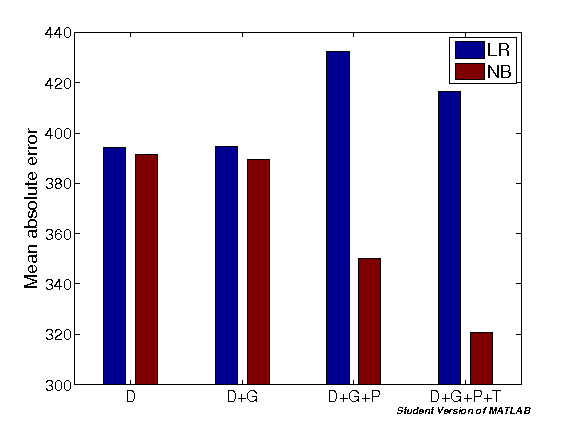
\includegraphics[width=0.8\textwidth]{fig/lrvsnb.png}
\caption{The inference error for linear regression base model. $^*$D -- demographic features, G -- geographical influence, P -- POI features, T -- taxi flow feature}
\label{fig:lrvsnb}
\end{figure}



It is clear that the negative binomial model significantly outperform the linear regression model. Meanwhile, the negative binomial model captures our intuition well. Namely, adding new features will effectively improve the estimation accuracy.


In Table~\ref{tb:perf},  we can see that in different years and under most settings, the negative binomial regression significantly outperforms the linear regression (with only a few exceptions when using only demographic feature). When using all the features, NB is significantly better than LR with at least $6\%$ improvement in relative error.
One reason is that the negative binomial is a count prediction model, which assumes some distribution for the predicted variable and guarantee its positivity. Another reason is that it is difficult to get very precise estimation of crime rate, and  negative binomial model allows a large variance in the estimated crime rate. Therefore negative binomial is more appropriate for crime rate estimation than linear regression.





\section{Conclusion}


In this chapter, we discuss the a general inference problem that using information on the links to understand the nodes.


We extend the spatial autoregressive model in the literature by adding new types of flow into the model.  We call this model flow augumented spatial autoregressive model. This modification makes it impossible to use standard T-test to get the significance of the model coefficients. Therefore, we use the Monte-Carlo tests, where a repeated leave-one-out schemes is designed.


The flow augumented spatial autoregressive model has its own weakness, which will be discussed in next chapter. In the next chapter, we presents the unified graphical model to model the interactions.

\chapter{A Unified Graphical Model}

\label{ch:crf}


In this chapter, we propose to use a unified graphical model to model the interactions among regions. We start from a discussion on the major flaw of previous flow augmented spatial autoregressive model, that as a global spatial model is assumes spatial stationarity. However, in the real problem there is usually a spatial non-stationarity over some properties. For example, we observe that the relationship between crime count and total population in each community presents such spatial non-stationarity.

To fix the spatial non-stationarity issue, the most widely used method is called \emph{geographically weighted regression} (GWR) in the literature. In the next section, we will discuss the pros and cons to employ GWR to capture the spatial non-stationarity. Since our problem has multiple ``hyperlink'' flows in addition to space continuity, the idea of GWR must be generalized over a high dimension space consisted of multiple interactions. However, this generalization is non-trivial, and thus we propose a graphical model to address this challenge.



The graphical model is a natural way to capture the complicated interactions among regions.
With the same graphical model, we further show that other data mining tasks in urban space can be solved as well.  Therefore, we believe this graphical model is superior than other model in capturing the interactions, which consequently could be a united model.



\section{Capture Spatial Non-stationarity}

\subsection{Global Model vs. Local Model}

\begin{figure}[h]
\centering
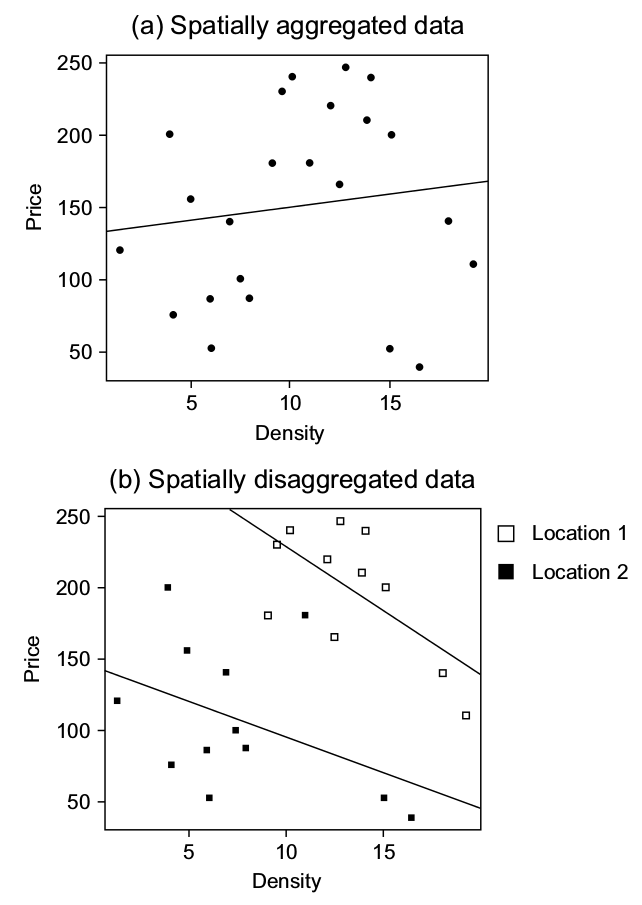
\includegraphics[width=0.7\textwidth]{fig/simpson.png}
\caption{A spatial example of Simpson's Paradox (from~\cite{GWR03}).}
\label{fig:simpson}
\end{figure}

\begin{figure}[h]
\centering
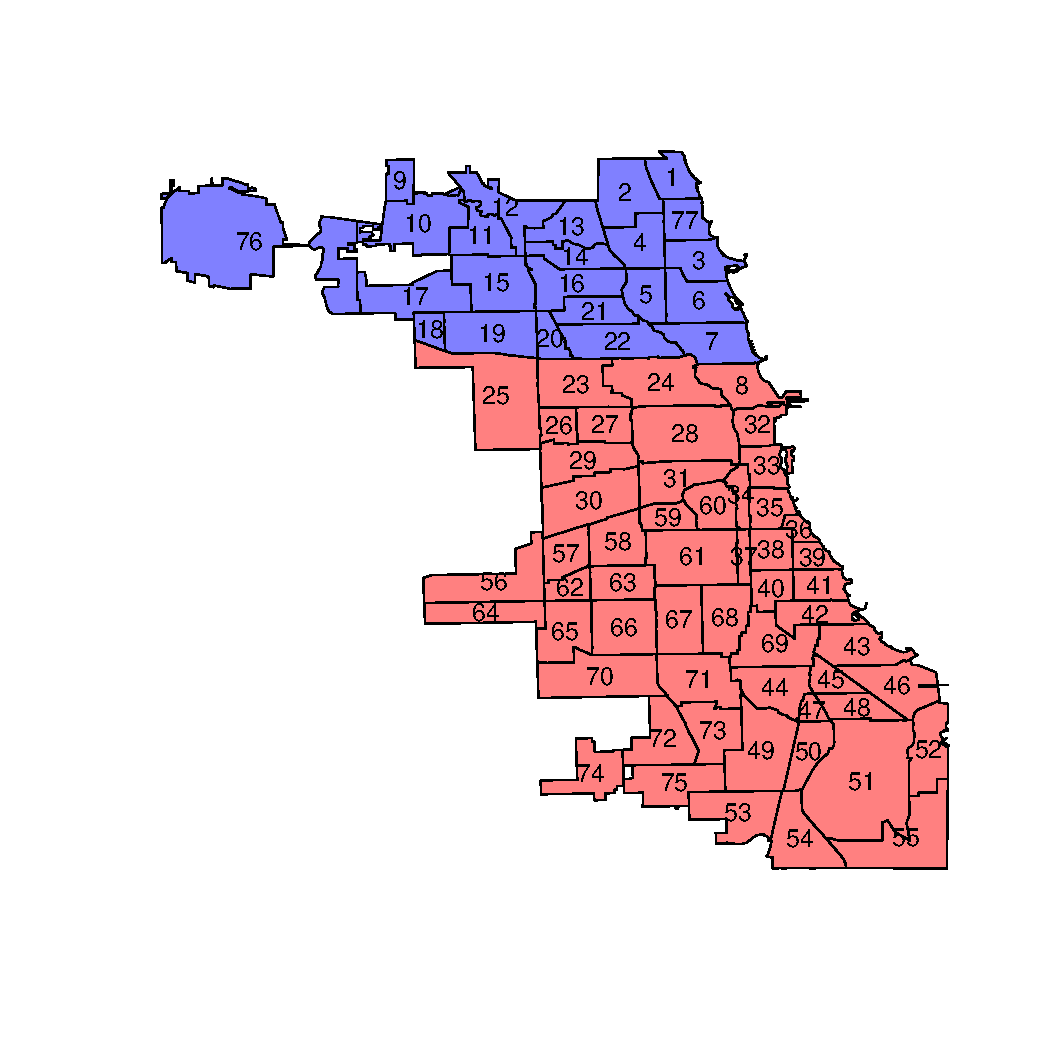
\includegraphics[width=0.45\textwidth]{fig/north-south-split.pdf}
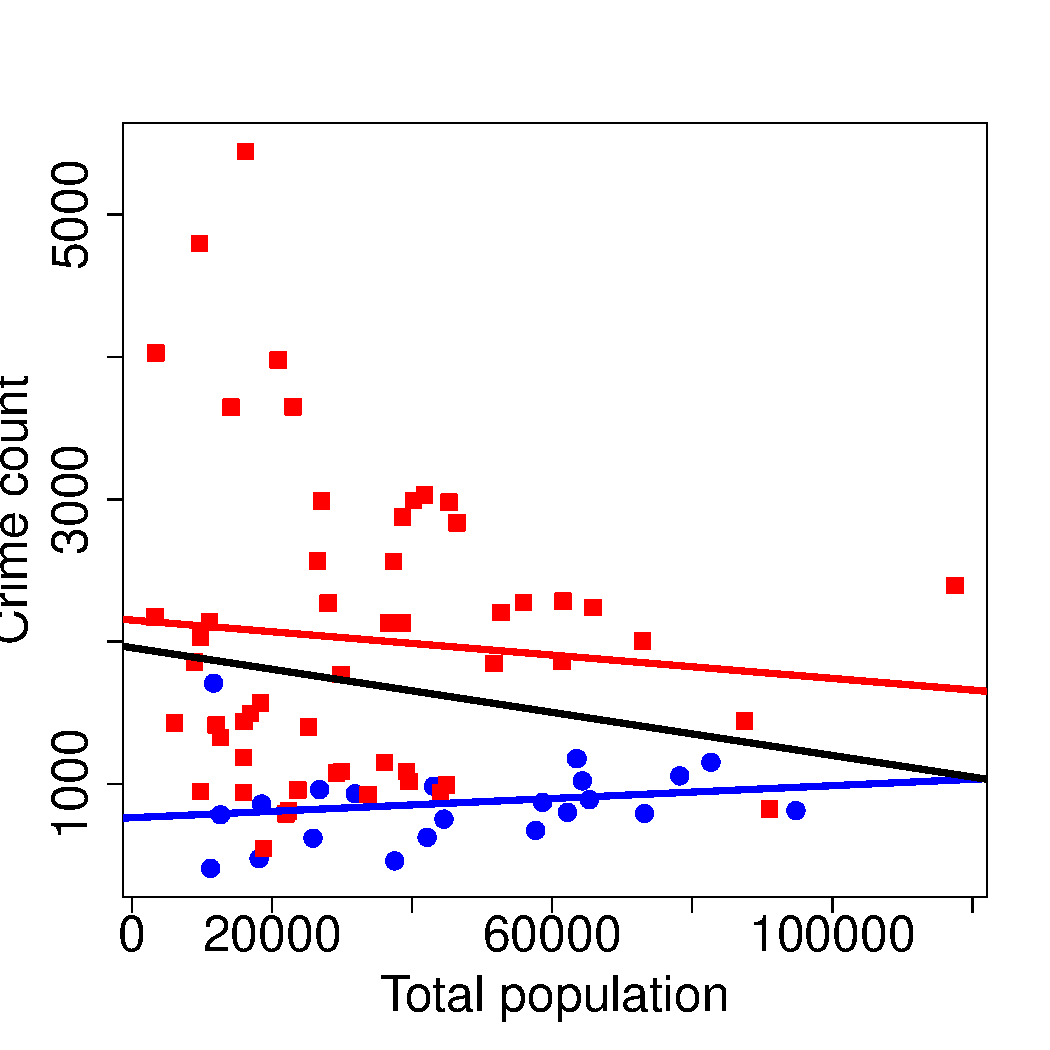
\includegraphics[width=0.45\textwidth]{fig/crime-pop.pdf}
\caption{The crime count vs. total population relationship shows spatial non-stationary property.}
\label{fig:spa-non-sta}
\end{figure}


Global model assumes the statistical relationships does not change over space. However, some statistical relationship is not stationary over space, which requries specific treatment for different locations, i.e. a local model at different places.



According to \cite{GWR03}, using global estimates of statistics can present misleading interpretations of local models. This is shown as an example in Figure~\ref{fig:simpson}, known as Simpson's Paradox~\cite{wiki:simpson}. The reason of Simpson's Paradox is that there is a hidden distribution of properties over space, which leads to opposite results in global model when aggregate subgroups over space.





In the Chicago crime inference example, we also observed similar phonomenon, as shown in Figure~\ref{fig:spa-non-sta}. We divide Chicago into two half: i) downtown north, ii) downtown and downtown south. The intuition is that the Chicago south usually have more crime than north, therefore we want to split Chicago into low-crime half and high-crime half. The splition of Chicago communites are visualized in left figure of Figure~\ref{fig:spa-non-sta}. 
On the right of Figure~\ref{fig:spa-non-sta}, we present the total crime plotted against total population. It is clear that in the high-crime half of Chicago the relation is almost neutral (coefficient as 0), and in the low-crime half of Chicago the relation is postive. However, the global model (black line) presents a negative correlation.





\subsection{An Existing Solution: Geographically Weighted Regression}


Geographically weighted regression (GWR) is a term introduced in \cite{GWR03} to describe a family of regression method in which the coefficients $\beta$ are allowed to vary spatially. GWR uses the coordinates of each sample or zone centroid $t_i$, as a target point for a form of spatially weighted least squares regression. The model is of the form:

\begin{equation}
y = X \beta(t) + \epsilon
\end{equation}

The coefficient $\beta(t)$ are determined at different regression point locally by its neighboring sample points. A weighting schema or spatial kernel $W$ is employed to weight neighboring sample points accordint to its distance to regression point. The Figure~\ref{fig:spa-kernel} is an example of the weighting function.


\begin{figure}[h]
\centering
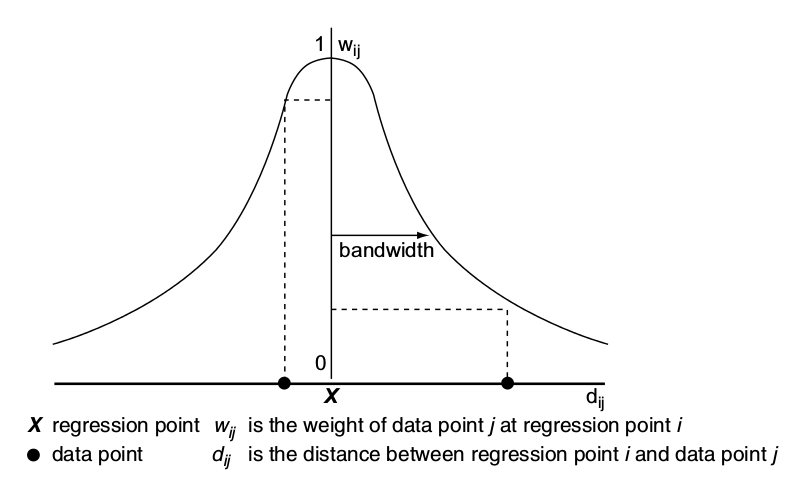
\includegraphics[width=0.8\textwidth]{fig/spatial-kernel.png}
\caption{A spatial kernel. Example from ~\cite{GWR03}}
\label{fig:spa-kernel}
\end{figure}



The GWR idea is able to be applied on top of spatial autoregressive (SAR) model, so that SAR model deals with spatial non-stationarity.  In the next we discuss another similar model called adaptive spatial model. After that, we discuss a common drawbacks of this two models.


\subsection{An Alternative Solution: Adaptive Spatial Model}


We use various types of data to estimate the crime count in community area (CA) of Chicago. For each CA we have observations on crime count and demographics. For each pair of CAs we also have observations on the taxi flow and spatial distance. One straightforward method is to build a regression model from all the features we observed to the crime counts.

We have one interesting observations is that in the south and north part of Chicago, the significance of different features are different. Therefore, the idea is to learn a dynamic weights for different spatial region.



Suppose we have $n$ regions in total, $R = \{ r_1, r_2, \cdots, r_n \}$.
The following notations are used

\begin{table}[h]
\centering
\begin{tabular}{|l|r|}
\hline
crime count at $r_i$ & $y_i$ \\ \hline
demographics at $r_i$ & $\mathbf{d}_i$ \\ \hline
taxi flow between $r_i$ and $r_j$ & $f_{ij}$ \\ \hline
taxi flow weight matrix for $r_i$ & $\mathbf{f_i}$ \\ \hline
spatial weight matrix for $r_i$ & $\mathbf{g_i}$ \\ \hline
social flow lag variable for $r_i$ & $s_i = \mathbf{f}_i^T \mathbf{y}$ \\\hline
spatial flow lag variable for $r_i$ & $p_i = \mathbf{g}_i^T \mathbf{y}$ \\\hline
\end{tabular}
\caption{Symbols for the dynamic coefficient model.}
\end{table}


\textbf{Dynamic linear regression model}



For simplicity we use linear regression model
\[
y_i = \mathbf{w}_1^T \mathbf{d}_i + w_2 s_i + w_3 p_i + w_4,
\]
where $\{ w \}$ are the coefficients.

To simplify notations, we use $\mathbf{x}_i$ denote all the available predictors for region $r_i$,
\[
\mathbf{x}_i = [ \mathbf{d}_i, s_i, p_i, 1 ].
\]
Then the model becomes 
\[
y_i = \mathbf{w}^T \mathbf{x}_i.
\]



Now we use a dynamic model, where $\mathbf{w}$ is different for various regions.
This leads to 
\[
y_i  = \mathbf{w}_i^T \mathbf{x}_i.
\]


The problem with formulation is that there are too many parameters to learn. To address this issue, we use the constraint that \textbf{spatially adjacent regions share similar coefficients}.

We use $S_{ij}$ to denote the adjacency of $r_i$ and $r_j$. And the aforementioned constraint is formulated as
\[
\min \sum_{i,j} S_{ij} ||\mathbf{w}_i^T - \mathbf{w}_j^T||_2^2
\] The several choice of $S_{ij}$
\begin{itemize}
\item Binary indicator. $S_{ij} = 1$ if two regions are contiguous, otherwise $S_{ij} = 0$.
\item The reverse distance between $r_i$ and $r_j$. 
\end{itemize}

The overall objective is

\begin{equation}
\label{eq:obj}
\min_{\mathbf{W}}  \sum_i || y_i - \mathbf{w}_i^T \mathbf{x}_i ||_2^2 + \eta \sum_{i,j} S_{ij} ||\mathbf{w}_i^T - \mathbf{w}_j^T||_2^2 
+ \theta || \mathbf{W} ||_F^2
\end{equation}




\textbf{Optimization}


Rewrite the Frobenius norm in the last term
\[
|| \mathbf{W} ||_F^2 = \sum_i || \mathbf{w}_i - \mathbf{0}||_2^2.
\]


Therefore the Equation~\ref{eq:obj} is rewritten as
\begin{equation}
\label{eq:obj2}
\min_{\mathbf{W}}  \sum_i || y_i - \mathbf{w}_i^T \mathbf{x}_i ||_2^2 + \eta \sum_{i,j \in 0, \cdots, N} S_{ij} || \mathbf{w}_i - \mathbf{w}_j ||_2^2,
\end{equation}
where $\mathbf{w}_0 = \mathbf{0}$ and $S_{0i} = 1$ for $\forall i$.


To solve the objective in Equation~\ref{eq:obj2}, we use variable splitting. Namely, when optimizing for $\mathbf{w}_i$, we assume all other $\mathbf{w}_{j, j\neq i}$ are fixed. The sub-problem is
\begin{equation}
\label{eq:subobj}
\min_{\mathbf{w}_i}   ||y_i - \mathbf{w}_i^T \mathbf{x}_i ||_2^2 + \eta \sum_j S_{ij}|| \mathbf{w}_i - \mathbf{w}_j||_2^2.
\end{equation}



The update on $\mathbf{w}_i$ is
\[
\mathbf{w}_i = \min_{\mathbf{w}_i}   ||y_i - \mathbf{w}_i^T \mathbf{x}_i ||_2^2 + \eta \sum_j S_{ij} || \mathbf{w}_i - \mathbf{w}_j^{(t)} ||_2^2.
\]

The closed-form solution is

\begin{equation}
\mathbf{w}_i = (\mathbf{x}_i^T \mathbf{x}_i + \eta \sum_j S_{ij} \mathbf{I} )^{-1} (y_i \mathbf{x}_i + \eta \sum_j S_{ij} \mathbf{w}_j) 
\end{equation}


\textbf{Inference}

We use the \textbf{leave-one-out} setting to infer and evaluate the crime rate of new community area. 

Suppose the we want to estimate the crime rate $y_i$ of $CA_i$. During the training process, we hold everything about $CA_i$ out (including $y_i$, flow coming in and leaving from $CA_i$). Then training the model on $CA_j$, $\forall j \neq i$, which gives us $w_j$, $\forall j \neq i$. To infer the $y_i$, we need estimate the model coefficient $w_i$ first. Follow the same intuition that model on $CA_i$ is only similar to all its neighboring models, we have
\begin{equation}
\min_{\mathbf{w}_i} \sum_{j, \forall j \neq i} S_{ij} || \mathbf{w}_i - \mathbf{w}_j ||_2^2 + || \mathbf{w}_i ||_2^2
\end{equation}

After getting $\mathbf{w}_i$, we infer $y_i$ by
\begin{equation}
\hat{y}_i = \mathbf{w}_i^T * \mathbf{x}_i
\end{equation}




\subsection{Comparison of GWR and Adaptive Model}


Both the GWR and Adaptive model address the spatial non-stationarity by building local models. Two models use different approaches to model the spatial continuity.

GWR implicitly model the spatial continuity by using similar sample points for two nearby regression models. Meanwhile, the adaptive model explicitly put a constrait to make two nearby models similar.

Both mehtods can be extened with newer type of interactions. We use $W^0$ denote the spatial adjacency matrix, and use $W^k$, $k = 1,2, \cdots$ to denote the interactions matrix of data type $k$. Therefore, we are extending the two dimensional distance weighting kernel into a high dimension distance measure. 


However, this high dimension distance measure is non-trivial to calculate. Suppose now we have taxi flow and LEHD flow in addition to geospatial adjacency. The tricky question to ask is which interaction is more important to connect two regions? We can give weight coefficient to different interactions, so that

\begin{equation}
W =  \alpha_0 W^0 + \alpha_1 W^1 + \cdots  +\alpha_k W^k
\end{equation}
where $\sum_0^k \alpha_i = 1$.

However, the $W$ in both GWR and adaptive model is pre-given. Therefore, incorporating heterogeneous flows is the major challenge of both GWR and adaptive model.




\section{Graphical Model to Capture Complicated Interactions}



The methods in the literature is not originally designed to handle heterogenous interactions among regions, and therefore have the major challenge mentioned above. The heterogenous interactions generate different network structure for us.  Therefore, we propose to model the interactions of two regions as a latent variables with a graphical model. 




\subsection{Problem Formulation}

We want to predict the crime rate $y_i$ of each geographical grid (tract/community area) $g_i$. The available observations are demographics features $\x_i$ of each $g_i$ from census, and the interactions among grids. We denote the interactions as $\f_{ij}$ for grid pair $g_i, g_j$, and examples of such interactions are social flow and geospatial distance.

\subsection{Conditional random field model}


\textbf{Potential Function}
Each grid is a node, and its crime rate $y_i$ is the hidden variable that we want to estimate. Two kinds of fixed parameters are observed for each grid $g_i$. The first one is the demographic features $\x_i$. The second is the interactions among grids, such as social flow and geospatial distance, denoted by $\f{ij}$.

We use Conditional Random Field (CRF) shown in Figure~\ref{fig:crf} to model the dependency of nodal features. The learning goal is to estimate the conditional probability of $y$ given $\x$ and $\f$

\begin{equation}
	P(y |  \x, \f) 
\end{equation}

This model can handle the spatial non-stationary issue, since we can learn the conditional probability separately at different locations.




\begin{figure}[hb]
	\centering
	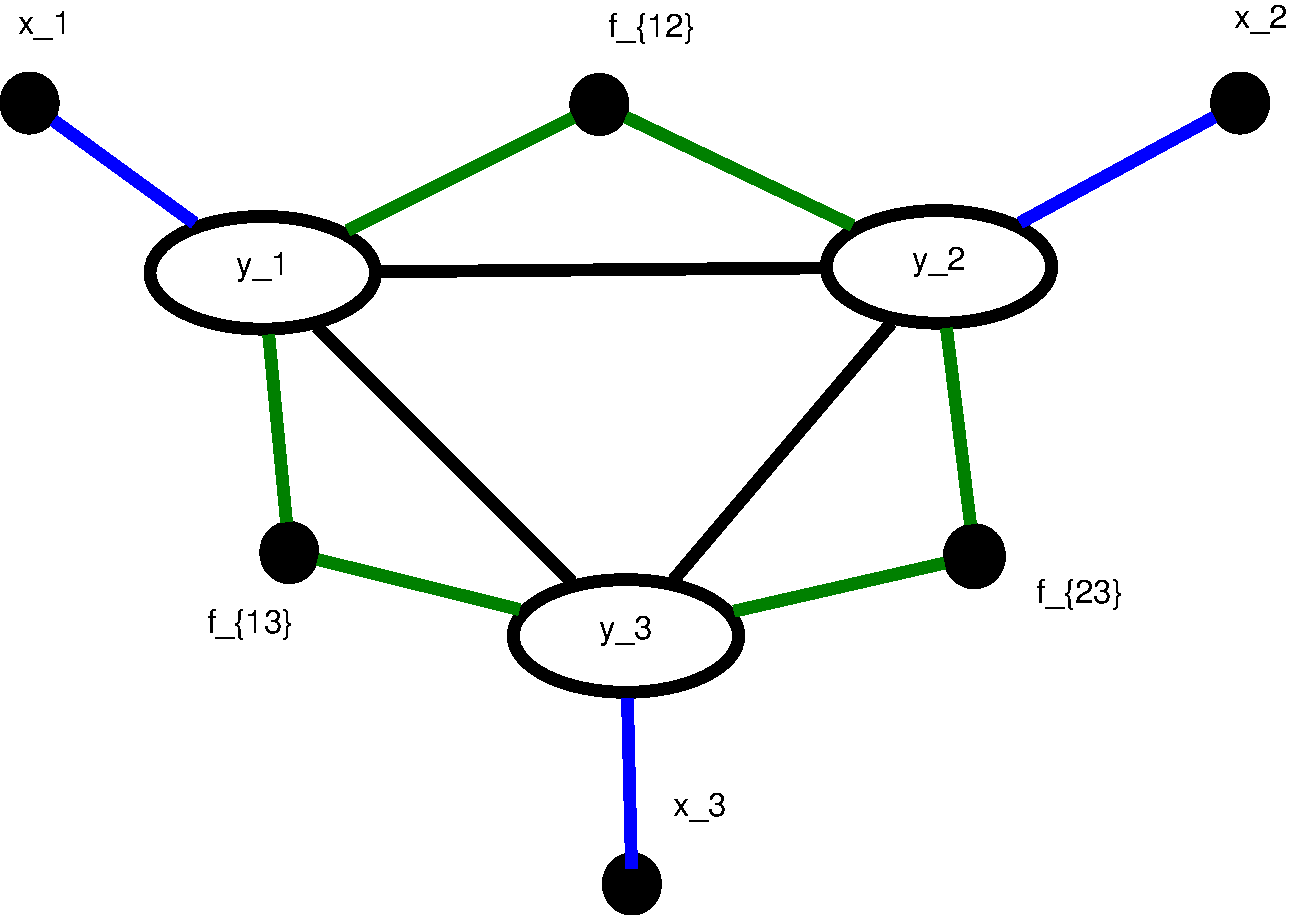
\includegraphics[width=0.5\textwidth]{fig/CRF-fig.pdf}
	\caption{The CRF model of the crime rate $y_i$ for each grid $g_i$.}
	\label{fig:crf}
\end{figure}



In the CRF model, we factorize the probability distribution of $y$ to a series of potential functions $\psi$ on the clique. 
\begin{equation}
	P(Y) = \frac{1}{Z} \prod_{ c \in C} \psi(c)
\end{equation}

Use $C_1$ to denote the set of cliques of size 1 with the form $\langle y_i \rangle$, and $C_2$ to denote size-2 clique. We define the potential function as follows:

\begin{align}
	\psi_{C_1} = &exp( - |y_i - \demow^T \cdot \x_i| )  \forall i \in [1, n], {g_i} \in C_1, \\
	\psi_{C_2} = & exp( - |y_i - y_j - \w^T \cdot \f_{i,j}| )  \forall i,j \in [1, n], {g_i, g_j} \in C_2, 
\end{align}
where $\demow$ and $\w$ are all positive coefficients.

The distribution of $Y$ is given by 
\begin{equation}
	P(Y) =  \frac{1}{Z} \left[ \prod_{i=1}^n \psi_{C_1}(y_i) \times \prod_{i=1}^n \prod_{j=i}^n \psi_{C_2}(y_i, y_j) \right]
\end{equation}
\begin{equation}
	P(Y) =  \frac{1}{Z} exp  \left( - \sum_{i=1}^n |y_i - \demow^T \cdot \x_i|  - \sum_{i=1}^n\sum_{j=i}^n |y_i - y_j - \w^T \cdot \f_{i,j}| \right)
	\label{eq:PY}
\end{equation}


The inference of $CRF$ model is given in the Appendix~\ref{apdx:crf}, and we refer interested reader there.




\section{Graphcial Model Solve Other Proposed Problems}



The graphical model is not only useful to solve inference problem on nodes using links, but also able to solve other problems.



\subsection{Understand links using nodes.}

In a graphical model shown in Figure~\ref{fig:crf}, we can estimate the flow $f_{ij}$ using the nodal attributes $y_i$ and $\x_i$ as well.


This problem answers important questions about the link. For example, we can answer when two regions are becoming very dissimilar in $\x$, what will happend to the taxi interaction between them? What about the LEHD flow.



\subsection{Understand the causal structures}


Graphical model also helps us understand the real dependency structure of node property and flow between nodes.
The assumptions that crime is neighboring community will influence crime in focal community is  over-simplified. Actually, we do not know what impacts crime in focal community. It is very likely to be nodal properties in neighboring communites that impacts crime in focal community. There are various explanations behind, as shown in Figure~\ref{fig:crf-assump}.



\begin{figure}[h]
\centering
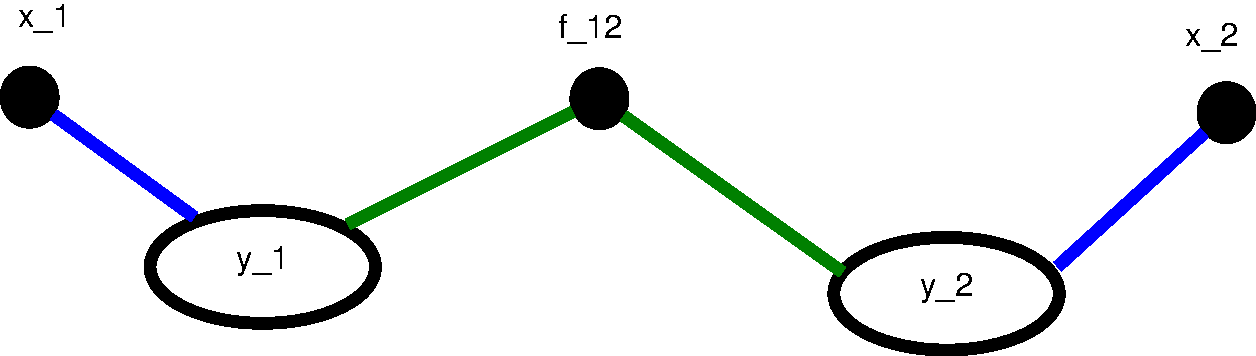
\includegraphics[width=0.45\textwidth]{fig/CRF-base.pdf}
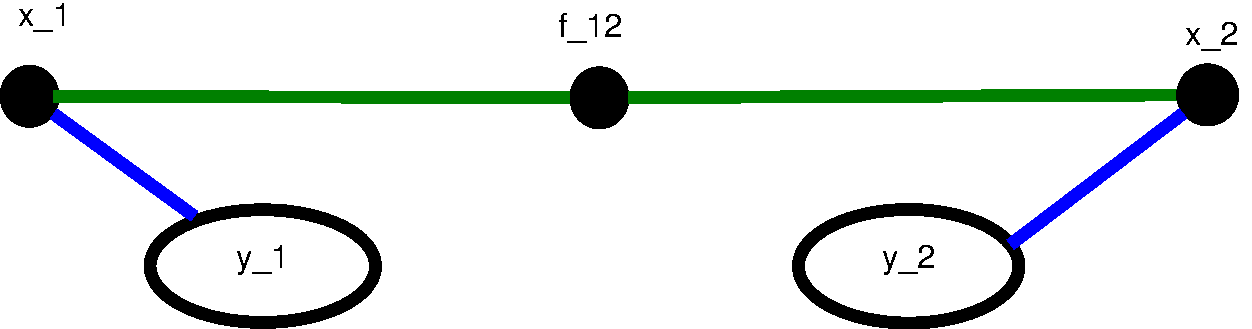
\includegraphics[width=0.45\textwidth]{fig/CRF-impr.pdf}
\caption{Various assumptions on interations behind the inference problem.}
\label{fig:crf-assump}
\end{figure}



%\chapter{Tackling Spatial Continuity: Task-Specific Region Partition}
\label{ch:partition}


% !TEX root =  main.tex
\section{Introduction}

% More data are available
Recent years have seen more and more cities join the open data initiative. For example, as of December 2016, more than 1600 data sets are available on  NYC open data catalog \cite{nyc-open-data}. These public urban data collectively reflect urban dynamics and provide a unique opportunity to fully engage the data-informed city. 

% model

Given the growing amount of urban data, a number of data-driven models have been developed to provide insights for urban problems. A frequent approach is to treat each region as a data sample, take the region properties as features, and build a model to learn the correlation between region features and a target variable. One common application lies in the domain of crime prediction. Criminologists are interested in knowing the correlation between demographics and crime~\cite{wang2016crime,wang2017non}. Each region $i$ is taken as a data sample, with $X_i$ as its demographic feature and $Y_i$ as its crime count. A model (e.g., linear regression or negative binomial model) is built to estimate crime count vector $Y$ using the feature matrix $X$. If some features (e.g., disadvantage index) show a significant correlation with crime count, researchers could relate this empirical result with criminology theory~\cite{graif2014urban} and policy makers could further propose corresponding policies to address crime issues.

Existing studies often use pre-defined administrative boundaries (e.g., street block, census tract, community area, or neighborhood) to define a region~\cite{yuan2012discovering,wang2016crime}. An example of the 77 administrative community areas of Chicago is shown in Figure~\ref{fig:intro}. However, such administrative boundaries might be too rigid and do not reflect the true spatial structure with regards to the targeted urban issues. For example, the definition of regions for crime study might be different from the regions used to understand real estate market. One can alternatively propose to study the problem at the point level or small grid cell level (e.g., 10 meters by 10 meters grids). However, this could lead to data sparsity issues and jeopardize the integrity of the statistical model. Consequently, any inference made from the model would be at risk of bias. These concerns have both theoretical and policy implications. We use the following example to further illustrate the issue of using pre-defined community areas to study crime.

\begin{figure}[t]
\centering
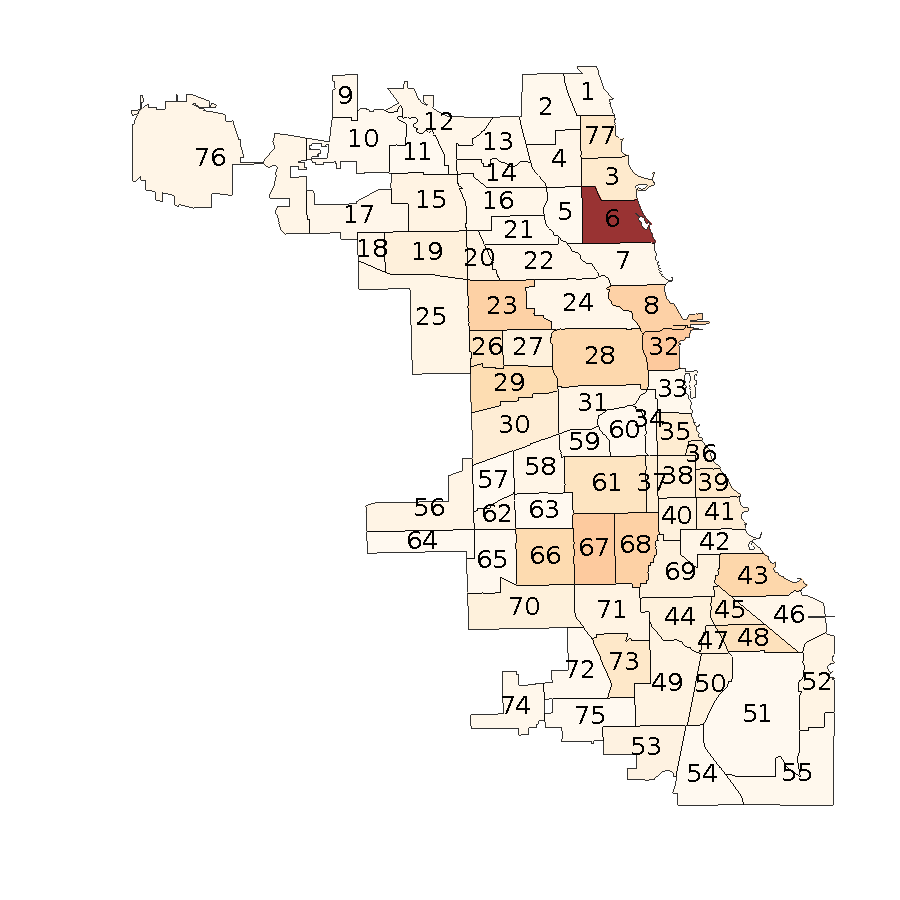
\includegraphics[width=0.4\linewidth]{fig/error_heatmap.pdf}
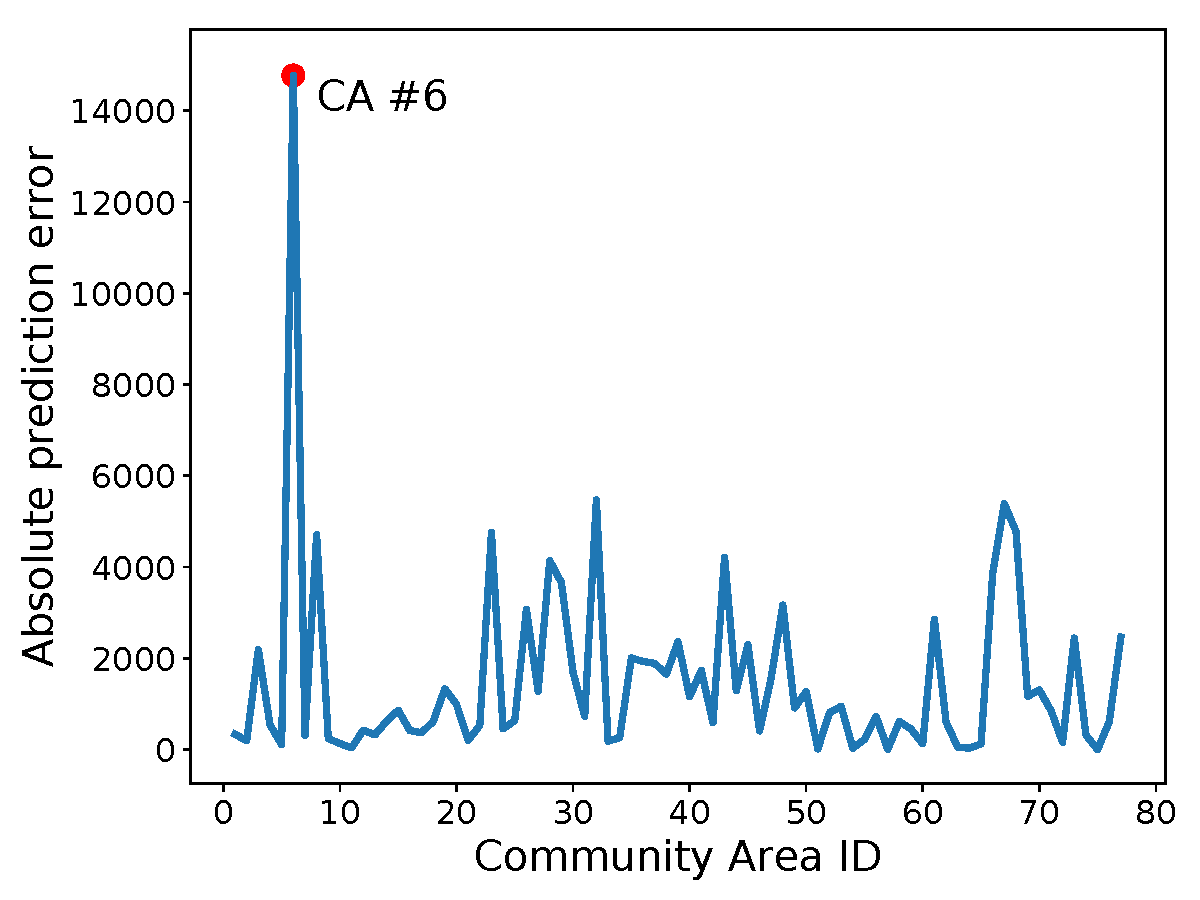
\includegraphics[width=0.5\linewidth]{fig/ca-abs-errors.pdf}
\caption{Crime prediction error at community level in Chicago. The community area \#6 is an outlier with a large error.}
\label{fig:intro}
\end{figure}

\begin{figure}
\centering
\subfigure[Census tracts of community \#6.]{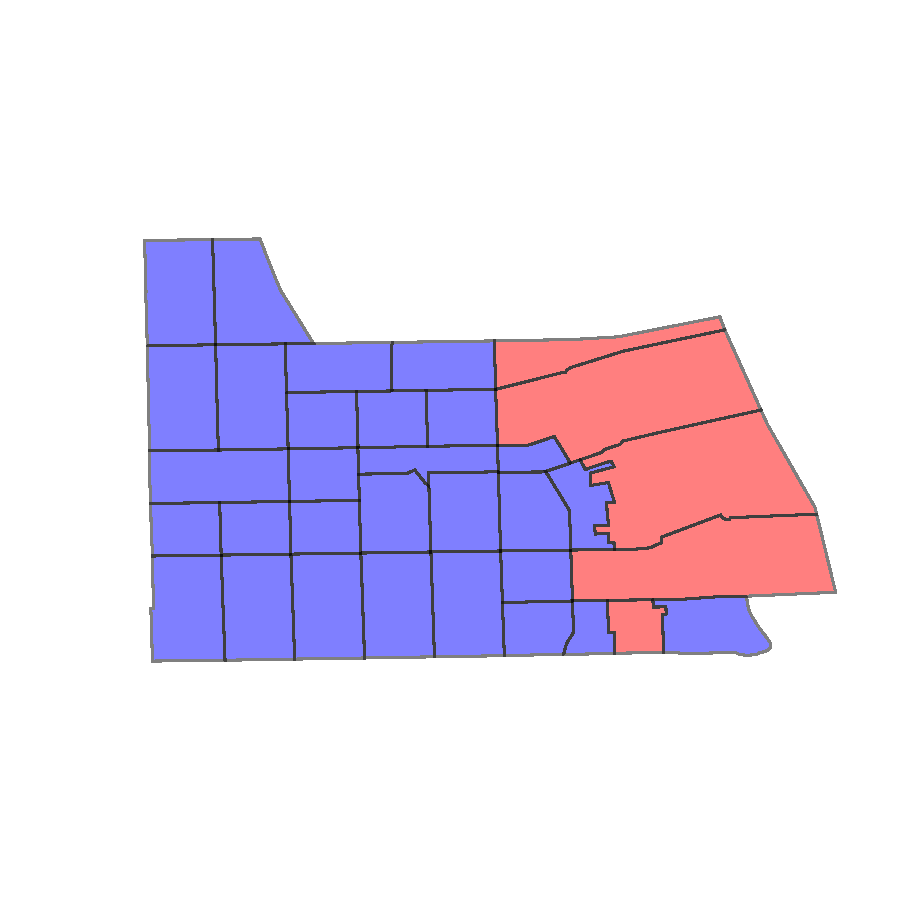
\includegraphics[width=0.5\linewidth]{fig/tracts_within_CA.pdf}}
\subfigure[Tract similarity.]{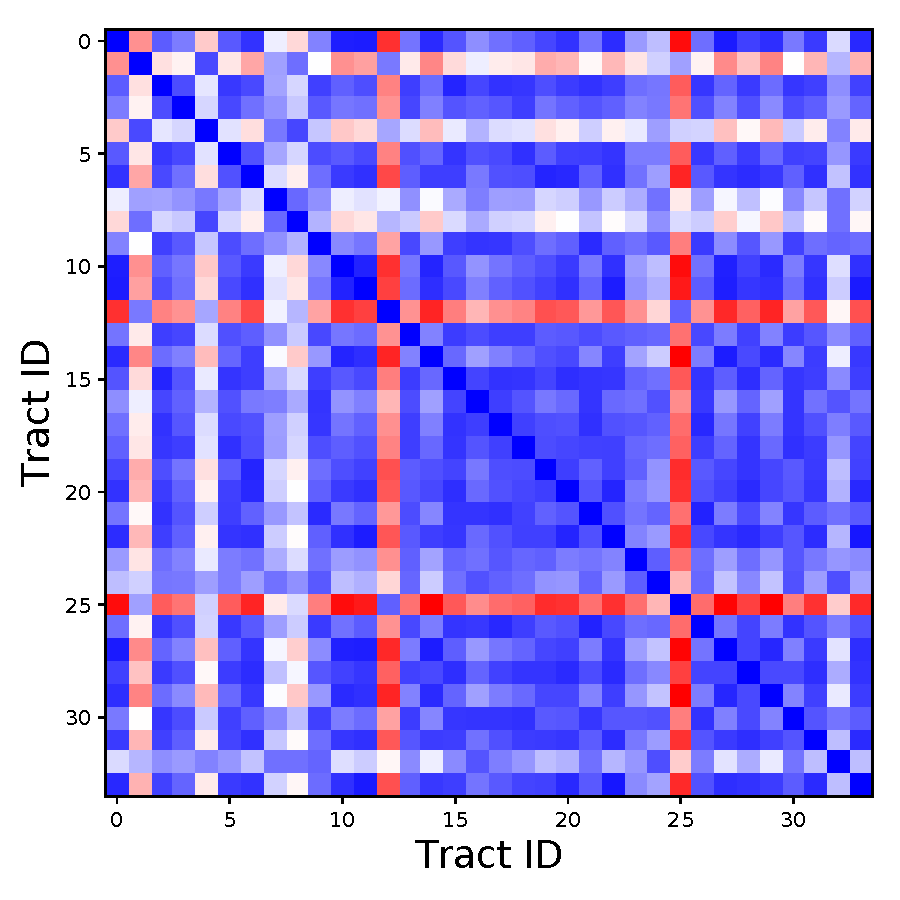
\includegraphics[width=0.45\linewidth]{fig/tract_sim_matrix.pdf}}
\caption{Explaining the outlying community area \#6 in Figure~\ref{fig:intro}. (a) Visualization of the 34 tracts in community \#6. (b) The pair-wise similarity of 34 tracts in terms of demographic features. It is clear that five tracts (in red color) on the east side are different from the other blue tracts.}
\label{fig:intro-explain}
\end{figure}

\begin{example}
Following previous work~\cite{wang2016crime}, we construct a negative binomial model to predict crime count using demographic features by treating each community area as a data sample. Figure~\ref{fig:intro} plots the crime prediction error for each community area of Chicago. Community area \#6 (i.e., Lake View area) shows an abnormally high error. In order to explain this outlier, we further investigate the internal structure of this area. Community \#6 consists of 34 census tracts as shown in Figure~\ref{fig:intro-explain}(a).  In Figure~\ref{fig:intro-explain}(b), we visualize  pair-wise Euclidean distance between tracts based on demographic features. There are five tracts that are different from the other tracts in the demographic feature space, and they are all located on the east side of community \#6. These five tracts, when mixed with other tracts in this community, lead to inferior performance of crime count prediction in that area. 
\end{example}

% problem definition
The observation above motivates us to learn a better region definition for crime study. In this chapter, we propose a new problem of \emph{task-specific region partitioning}. Given spatial variables and a selected model  (e.g., linear regression), we aim to partition the city into regions such that the model trained by taking regions as data samples achieves the optimal results.

% literature
%two lines of literature: (1) clustering, no target; (2) partition tracts into regions, and build a model for each region.
To the best of our knowledge, task-specific region partitioning is a new problem that has not been studied before. While there exist many methods for spatial clustering~\cite{miller2009geographic}, most of them group the locations based on the similarity of their spatial properties and do not have a target variable to predict. Another similar problem is to partition the locations into $k$ regions and fit a model for each region. Such a problem definition has a different purpose with the goal of showing that the correlations between features and target vary over the space (e.g., in some area, disadvantage index  correlates with crime; while in some other areas, it does not). In our problem definition, we aim to fit one model for the whole city hoping to get a generalized interpretation (e.g., disadvantage index significantly correlates with crime count in Chicago). Such a problem definition is a frequently adopted form in the criminology literature~\cite{graif2014urban}.

% challenge & proposed solution
Task-specific city region partitioning is a challenging problem. The key challenge lies in that the region properties (both features and target variable) and the model coefficients change simultaneously when we change the region partition. We prove that this is an NP-hard problem. In our proposed solution, we employ the Markov Chain Monte Carlo (MCMC) method. We start from a pre-defined region partition (e.g., community areas), and generate a new partition sample by flipping the membership of a smaller area (e.g., a tract). Two variants of MCMC methods are proposed to solve this problem. First, a naive MCMC method generates the next partition sample by randomly flipping a tract. Second, a heuristic-based MCMC method generates the next sample by flipping one tract randomly selected from the community areas with the highest error. Finally, we employ reinforcement learning to automatically learn how to generate the next sample that is more likely to improve the prediction performance.


% Experiments results
We evaluate our method on two real datasets, i.e. crime count and real estimate price. The learned region partitions are shown to consistently outperform the administrative boundaries and spatial clustering method. For example, our methods, on average, outperform the administrative boundary by $56\%$ in a crime prediction task. We also observe that the heuristic-based MCMC converges faster than the naive MCMC, while the reinforcement learning uses the least iterations to converge.

% Key contributions
To summarize, the key contributions of this chapter are:
\begin{itemize}[leftmargin=*]
\item We propose a novel problem on task-specific region partitioning. This problem is motivated by real-world urban studies, including our own previous work on crime prediction~\cite{wang2016crime}.
\item We prove the problem is NP-hard and we study different MCMC and reinforcement learning sampling techniques to solve the problem. 
\item We validate our method through extensive experiments on two real datasets.
\end{itemize}


% chapter organizations
The rest of this chapter is organized as follows. The formal definition of our problem is given in Section~\ref{ch4-sec:problem}, and our method is described in Section~\ref{ch4-sec:method}. Section~\ref{ch4-sec:experiment} shows the evaluations on two different tasks. Section~\ref{ch4-sec:related-work} summarizes related work.  Finally, we conclude in Section~\ref{ch4-sec:conclusion}.


\section{Related Work}
\label{sec:related-work}


\textbf{Urban Data Heterogeneity.} Various urban data exhibit high degrees of correlation. As we collect more types of new urban data, we are able to solve a wide spectrum of urban problems. For example, a real-time air quality inference system is proposed in \cite{zheng2013u}, which uses not only historical air quality data, but also traffic flows, structure of roads, and POIs. Zheng et. al.~\cite{zheng2014diagnosing} diagnose New York City noise pollution with complaint records, road networks, and human check-ins. Real estate values are predictable given online user reviews~\cite{fu2014sparse} and offline human mobility data~\cite{wang:region}. Wang et. al.~\cite{wang2016crime, wang2017non} improve crime prediction accuracy by combining POI data and taxi flow data.

These existing works focus on mining the subtle correlations across different domains of data. We generalize the urban problems above as a learning task ,$f$, which maps some urban features to a target variable of interest. In this paper, we use crime prediction and average house price prediction as two examples. We study how to define the domain of urban problem, $f$, because only when $f$ is defined over a proper unit of study (e.g. community areas), the learned correlation is consistent and significant. \\

\noindent\textbf{Traditional Region Partition Methods.} Our problem falls into the region segmentation category. There are four main types of region partition methods that are widely used in the urban computing literature. First, a fixed sized grid is the most straightforward partition for travel time prediction~\cite{wang2016simple}, interpret traffic dynamics~\cite{wu2016interpreting}, and air quality inference~\cite{zheng2013u}. Second, existing administrative boundaries are also used for crime prediction~\cite{wang2016crime}. Third, clustering of point-wise urban data to get regions. For example, Li et. al.~\cite{li2015traffic} study the bike-sharing system and propose to estimate the supply/demand of bikes in a station cluster. Finally, other partitions are specifically designed for special needs. For example, Yuan et. al.~\cite{yuan2012discovering} employ the major road networks to partition a city into regions and learn the function of each region. Xu et. al.~\cite{xu2017understanding} partition a city by cellular tower coverages to study the mobile traffic pattern in urban environment. Zheng et. al.~\cite{zheng2015forecasting} use fan-shaped partitions to predict fine-grained air quality, because wind direction is an important indicator.


While various partition methods are used in existing urban problems, none of the partition methods explicitly take the learning task $f$ into consideration. It is worthy mentioning that most existing partition methods are purely based on cartographic information, and do not make use of the urban data properties. In this paper, we try to partition the city with an explicit objective. \\


\noindent\textbf{Discrete Optimizations.} The objective of our problem is a discrete optimization problem and is easy to derive. However, since the problem is NP-complete, it is challenging to efficiently find an optimal solution. MCMC sampling has been shown to be effective in optimizing discrete structures~\cite{strens2003evolutionary}. We follow this line of work and propose to use MCMC sampling to search for the optimal partition. During the MCMC sampling process, a lot of partitions are sampled but do not achieve better prediction results. To solve this issue, we follow the learning to optimize technique~\cite{li2016learning}, and propose to employ the reinforcement learning framework to learn where to sample the next partition that is most likely to improve the learning task, $f$.
\section{Region Partition Problem}
\label{ch4-sec:problem}

In this section, we first present the formal definition of our method. Then we prove that this partition problem is NP-hard.


The input of our problem is a set of minimum spatial units. Without loss of generality, we use tract as the unit of study in this paper, and the set of tracts is denoted as $\mathcal{T} = \{ t_1, t_2, \cdots, t_n \}$. Within each tract $t_i$, the following information are available $\langle p_i, y_i, x_i \rangle$, where $p_i$ is a sequence of GPS coordinates representing tract exterior boundary, $y_i$ is the target variable of interest, such as crime count and average house price, and $x_i \in \mathcal{R}^d$ is a $d$-dimension contextual feature vector. Note that each tract is a polygon with one connected component.

We define community area as the proper unit to study the correlation between $y$ and $x$.
\begin{definition}[Community area]
 Each community area consists of several adjacent tracts, denoted as $Z_j = \{t_1^j, t_2^j, \cdots \}$. We derive $\langle P_j, Y_j, X_j \rangle$ for each community area $Z_j$ by aggregating $\{ \langle p_i, y_i, x_i \rangle | t_i \in Z_j \}$, where $P_j$ is the exterior boundary, $Y_j$ is the crime count, and $X_j$ is the contextual features of $Z_j$.
\end{definition}
Note that there are various approaches to aggregate tract-level features $x_i$ into community area features $X_j$. For example we can use element-wise summation, min, or max on categorical count features. We can also calculate entropy to derive a diversity feature as $X_j$.

With the definition of community area, we define the partition of a city.
\begin{definition}[Partition]
\label{def:partition}
A partition over $\mathcal{T}$ is denoted as $\mathcal{Z} = \{ Z_1, Z_2, \cdots, Z_m\}$, satisfying the following four conditions
\begin{enumerate}
\item (subset) $\forall j$, $Z_j \subset \mathcal{T}$;
\item (non-overlapping) $\forall p, q$, $Z_p \cap Z_q = \emptyset$;
\item (completeness) $\bigcup_{j=1}^m Z_j = \mathcal{T}$;
\item (spatial-continuity) $\forall j$, $P_j$ defines a polygon with exact one connected component.
\end{enumerate}
\end{definition}

A task is defined on a given partition of the city, where we aim to learn the correlation between $X$ and $Y$ at the community area level.
\begin{definition}[Task]
Given a partition $\mathcal{Z}$, a task is to learn a linear function $f$, such that $Y_j = f(X_j)$, 
where $X_j$ and $Y_j$ are target variable and contextual features of community area $Z_j$.
\end{definition}


Our ultimate goal is to have a more accurate prediction. The task-specific region partition problem is defined as follows.
\begin{definition}[Task-specific region partition]
\label{def:opt-problem}
Given a set of tracts $\mathcal{T}$ and a task $f$, find a partition $\mathcal{Z}$ with $m$ components, such that the task error is minimized. Formally, we have
\begin{equation}
\label{eq:objective}
\arg\min_{\mathcal{Z}, f} \sum_{j=1}^m \Big(||Y_j - f(X_j)||_2 + G(Z_j)\Big),
\end{equation}
where $G(\mathcal{Z}) = \sum_{j=1}^m G(Z_j)$ is a constraint function on partition.
\end{definition}

The constraint function $G$ ensures the partition $\mathcal{Z}$ has desirable property, such as small variance in community populations or balanced size in terms of community area. \\


\noindent\textbf{NP-Hardness}. The problem in Definition~\ref{def:opt-problem} is a combinatorial optimization problem, where the set of instances is $\mathcal{T}$, the feasible solution is $\mathcal{Z}$, and the quality measure of solution is $\mathcal{F}(\mathcal{Z}, f) = \sum_{j=1}^m \mathcal{F}(Z_i, f)$. The decision version of the problem is to find a partition $\mathcal{Z}$, such that $\mathcal{F}(\mathcal{Z}, f) \leq \epsilon$, where $\epsilon$ is a constant. In this section, we prove such decision problem is NP-complete, and therefore the optimization problem in Definition~\ref{def:opt-problem} is NP-hard.

In the NP-completeness proof, we approximate the decision problem above with an easier problem. The reason is that both $X_i$, $Y_i$, and $f$ are dynamically changing according to $\mathcal{Z}$, which complicates the original problem. First, we replace the jointly learned optimal $f$ with a fixed $f_0$. Since $f$ is optimal to minimize Equation~\ref{eq:objective} while $f_0$ is not, we have $\mathcal{F}(\mathcal{Z}, f) < \mathcal{F}(\mathcal{Z}, f_0)$. Second, we use $\sup \{\mathcal{F}(Z_j, f_0) \}$, where $\sup$ calculates supremum of a set, to approximate $\mathcal{F}(\mathcal{Z}, f_0)$. Since there are finite number of tracts within each community $Z_j$, and the task function $f_0$ can be solved in polynomial time, therefore the upper bound of $\mathcal{F}(Z_j, f_0)$ exists and is finite. Combine two approximations above, we have $\mathcal{F}(\mathcal{Z}, f) < m \cdot \sup \{ \mathcal{F}(Z_j, f_0)\}$. The approximated decision problem is to find a partition $\mathcal{Z}$, such that $m \cdot \sup \{\mathcal{F}(Z_j, f_0) \} \leq \epsilon_0$.

Now we prove the approximated decision problem is NP-complete. First, such approximated decision problem is NP, because given a partition $\mathcal{Z}_0$, we are able to validate $m \cdot \sup \{ \mathcal{F}(Z_j, f_0)\} \leq \epsilon_0$ in polynomial time. Next, we prove the NP-hardness of this problem by reducing the $(k,v)$-balanced partitioning problem to the approximated decision problem. The $(k,v)$-balanced partition problem~\cite{andreev2006balanced} is a proved NP-complete problem, which partition graph into $k$ disjoint components of size at most $v\frac{n}{k}$, while the capacity of edge cut is less than $\epsilon_0$. We construct the adjacency graph of all tracts $\mathcal{T}$, with weight $\sup \{\mathcal{F}(Z_j, f_0) \}$ on each edge. A solution to $(m,v)$-balanced partition problem on such adjacency graph is a solution to the approximated decision problem. The balanced partition problem achieve $k \cdot \sup \{\mathcal{F}(Z_j, f_0) \} \leq \epsilon_0$, where $k$ is the number of edges to cut the graph. It is clear that $k > m$, and therefore we find a partition satisfying $m \cdot \sup \{ \mathcal{F}(Z_j, f_0)\} \leq \epsilon_0$. 

The original problem in Definition~\ref{def:opt-problem} is NP-hard. Therefore, it is difficult to efficiently search for the optimal partition. In this paper, we use Markov Chain Monte Carlo sampling strategy to search for local optimal solutions.

\section{methods}
\label{sec:method}

In this section, we use the stochastic Markov Chain Monte Carlo (MCMC) method to automatically learn the partition $\mathcal{Z}$. We propose two variations of MCMC sampling method with different sample proposal strategy. And finally, we use reinforcement learning to make the best of historical samples and automatically learn the sample strategy.


\subsection{Markov Chain Monte Carlo}

There are two parameters, $\mathcal{Z}$ and $f$, to learn in Equation~\ref{eq:objective}. However, given a fixed partition $\mathcal{Z}$, the optimal task function $f$ can be easily learned. The challenge lies in searching through the partition space. Toward this goal, we adopt the MCMC method, or more specifically the Metropolis-Hastings algorithm to optimize $\mathcal{Z}$. 

Markov Chain Monte Carlo~\cite{andrieu2003introduction} is a stochastic algorithm for obtaining a sequence of random samples from a distribution for which direct sampling is difficult. A key property of the algorithm is that it constructs a Markov chain that will ultimately converge to $p$ through stochastic sampling \cite{ml:murphy}. In our case, the state space is all possible partitions $\mathcal{Z}$, and the distribution $p(\mathcal{Z})$ defines the probability that $\mathcal{Z}$ is optimal to Problem~\ref{def:opt-problem}. Clearly, it is difficult to calculate $p(\mathcal{Z})$, however the quality measure $\mathcal{F}(\mathcal{Z})$ is proportional to $p(\mathcal{Z})$. Namely, a partition $\mathcal{Z}$ with lower $\mathcal{F}(\mathcal{Z})$ value is more likely to be optimal.


In addition to the quality function $\mathcal{F}$, MCMC employs a proposal function $q(\mathcal{Z}'|\mathcal{Z})$, which defines the transition probability from state $\mathcal{Z}$ to $\mathcal{Z}'$. The Markov chain moves toward $\mathcal{Z}'$ with acceptance probability $\gamma$, defined as
\begin{equation}
\gamma = \min \Big [ 1, \frac{p(\mathcal{Z}')q(\mathcal{Z}| \mathcal{Z}')}{p(\mathcal{Z})q(\mathcal{Z}'|\mathcal{Z})} \Big ].
\label{eq:gamma}
\end{equation}

$p(\mathcal{Z})$ is the Boltzmann distribution, defined by
\begin{equation}
p(\mathcal{Z}) = \frac{e^{-\mathcal{F}(\mathcal{Z})/T}}{P}, 
\label{eq:boltzmann}
\end{equation}
where $P$ is the normalization constant, and $T$ is the temperature parameter. We do not explicitly compute $P$, because they cancel out in Equation~(\ref{eq:gamma}).

\begin{algorithm}
\caption{MCMC method to search $\mathcal{Z}$.}
\label{alg:mcmc}
\begin{algorithmic}[1]
\State $\mathcal{Z} \gets \mathcal{Z}_0$
\While {$\mathcal{F}(\mathcal{Z}) \geq \epsilon$}
  \State Sample $u \gets \mathcal{U}_{[0,1]}$
  \State Sample $\mathcal{Z}' \gets q(\mathcal{Z}'|\mathcal{Z})$
  \State $\gamma = \min \Big [ 1, \frac{p(\mathcal{Z}')q(\mathcal{Z}| \mathcal{Z}')}{p(\mathcal{Z})q(\mathcal{Z}'|\mathcal{Z})} \Big ]$
  \If {$u < \gamma$}
    \State $\mathcal{Z} \gets \mathcal{Z}'$
  \EndIf
\EndWhile
\end{algorithmic}
\end{algorithm}

The MCMC algorithm is shown in Algorithm~\ref{alg:mcmc}. First, we initialize the partition with the existing administrative boundary, denoted as $\mathcal{Z}_0$. Within each step, we draw $u \in [0,1]$ from uniform distribution $\mathcal{U}_{[0,1]}$, and draw the next partition $\mathcal{Z}'$. The acceptance probability $\gamma$ is calculated according to Equation~\ref{eq:gamma}. If $u$ is smaller than the acceptance probability $\gamma$, then we accept the new partition $\mathcal{Z}'$. We repeat the process above, until $\mathcal{F}(\mathcal{Z})$ converges.



\subsection{MCMC with Naive Proposal Distribution}

The proposal function $q$ is very flexible, if not limitless. In practice, the exact form of $q$ generally affects the efficiency of the algorithm, or how quickly it will converge. We begin by establishing a baseline MCMC approach to the region partition problem by outlining the simplest $q$ we can devise. 

We generate a new partition by randomly selecting one tract $t_i \in \mathcal{T}$ that is on the boundary of some community area $Z_j$, and then flip $t_i$ to the adjacent community area. Such a naive proposal function $q$ contains the following steps.
\begin{itemize}
  \item Maintain a set of tracts that are on partition boundary, denoted as $\mathcal{T}_b$.
  \item Uniformly draw $t_i$ from $\mathcal{T}_b$. The current community assignment for $t_i$ is $Z_j$. The probability of selecting $t_i$ is $1/|\mathcal{T}_b|$.
  \item Uniformly draw $Z_p$ from the set of adjacent community areas $Adjacent(t_i)$ of $t_i$. The probability of selecting $Z_p$ is $1/|Adjacent(t_i)$.
  \item Verify the four conditions in Definition~\ref{def:partition} are satisfied. If not, restart.
  \item Assign the $t_i$ to community $Z_p$. Update boundary set $\mathcal{T}_b$.
\end{itemize}

The naive proposal function $q$ is symmetric, because $q(\mathcal{Z}'|\mathcal{Z})=  q(\mathcal{Z}|\mathcal{Z}') = \frac{1}{|\mathcal{T}_b| \cdot |Adjacent(t_i|}$. Therefore, the acceptance probability $\gamma = \min[ 1, \frac{p(\mathcal{Z}')}{p(\mathcal{Z})}]$. 


\subsection{Guided MCMC with Softmax Proposal Distribution}

The naive proposal MCMC method is simple, but not efficient. The reason is that we are randomly trying different partitions. We now propose an MCMC approach with a more intelligent proposal strategy. This method follows a greedy intuition that we should adjust the community area with the highest prediction error to improve current partition.


Given this intuition, we heuristically design our guided MCMC method to sample a community area with large error first. To achieve this, we apply the softmax function over the prediction errors on community areas to derive the sample probability of each community area. The softmax proposal contains the following steps. 
\begin{itemize}
  \item Maintain a set of tracts that are on partition boundary, denoted as $\mathcal{T}_b$.
  \item Draw $Z_j$ from $\mathcal{Z}$ proportional to the prediction of error using softmax function, $p(Z_j) = \frac{ \exp(||Y_j - f(X_j)||_2) }{ \sum_{k=1}^m \exp(||Y_k - f(X_k)||_2)}$.
  \item Uniformly draw a tract $t_i$ from $Z_j \cap \mathcal{T}_b$.
  \item Uniformly draw $Z_p$ from the set of adjacent community areas $Adjacent(t_i)$ of $t_i$. The probability of selecting $Z_p$ is $1/|Adjacent(t_i)$.
  \item Verify the four conditions in Definition~\ref{def:partition} are satisfied. If not, restart.
  \item Assign the $t_i$ to community $Z_p$. Update boundary set $\mathcal{T}_b$.
\end{itemize}

Note that under the softmax proposal approach, the proposal function $q$ is not symmetric. Therefore, we have to explicitly calculate the values for $q$ function and plug into Equation~\ref{eq:gamma}.



\subsection{Reinforcement Learning}

There are two main drawbacks of the MCMC method. First, when drawing a new sample, the MCMC methods do not account for any information from previous samples.  For example, the naive proposal MCMC rejected early generations of samples, which do not contribute any information to future generations of samples. Intuitively, if we repeatedly observe that flipping some tracts give us lower gain, then we should lower the probability that such tracts are sampled again in the future. Second, the Markov chain-based stochastic search strategy is more likely to get stuck on a local optima. The reason is that the nature of MCMC sampling follows a depth first search in the huge search space. It is very likely that another chain exists that leads to a better local optima, but the algorithm is not able to achieve this better outcome.


To address the issues of the MCMC method, we further propose a reinforcement learning (RL)~\cite{sutton1998reinforcement} scheme for generating new samples. RL differs from standard supervised learning in that the correct input/output pairs are never presented. Instead, RL is concerned with how agents ought to take actions in an environment so as to maximize cumulative gain.

In what follows, we map the RL components to our problem. The set of tracts consists of the environment, and their community area assignment is the state. An action is to re-assign some tract $t_i$ from $Z_j$ to $Z_p$, denoted as tuple $\langle t_i, Z_p\rangle$. The immediate reward of such transition is defined by $\Delta \mathcal{F} = e^{-\mathcal{F}(\mathcal{Z}')} - e^{ -\mathcal{F}(\mathcal{Z})}$, where the exponential function coverts the loss into gain. We define the cumulative gain $Q$ as a function of the current state $\mathcal{Z}$ and action $\langle t^k, Z^k \rangle$ at step $k$, and $Q$ satisfies the following condition
\begin{equation}
\label{eq:Q-obj}
Q(\mathcal{Z}, \langle t^k, Z^k \rangle) = \Delta \mathcal{F} + \delta \cdot \sum_{a \in \{\langle t^{k+1}, Z^{k+1} \rangle\}} Q(\mathcal{Z}', a),
\end{equation}
where $\delta$ is the discount factor on future reward and $\{\langle t^{k+1}, Z^{k+1} \rangle\}$ is the set of all possible actions given $\mathcal{Z}'$. Given $Q$ function, at each state $\mathcal{Z}$, we are able to find the best action with a the highest cumulative gain through
\begin{equation}
\label{eq:Q-policy}
\arg\max_{\langle t, Z \rangle} Q(\mathcal{Z}, \langle t, Z \rangle).
\end{equation}


In our problem, a reinforcement learning scheme faces the following three challenges. We devise specific approximations to address these challenges. \\

\textbf{Huge state space}. The state space is exponential to the number of tracts. As a consequence, we cannot track the exact reward for each state and actions. Instead, we rely on Deep Q-learning~\cite{van2016deep}, where a deep neural network is learned to approximate the $Q$ function. Our neural network structure includes an embedding layer to encode the partition $\mathcal{Z}$ and action tuple, two dense fully connected dense layers, and finally the output layer predicts the sigmoid of $Q$.

\textbf{Large and dynamic action space}. The number of possible actions is linear to the number tracts. Also, for different partition states, the tracts on the boundaries are different, and thus the action set is also different. This property makes it difficult to calculate the summation of future $Q$ values in Equation~(\ref{eq:Q-obj}), and to find the maximum over all actions in Equation~(\ref{eq:Q-policy}). In this paper, we set the discount factor $\delta = 0$ to ease the calculation of $Q$. When searching for the best action with Equation~(\ref{eq:Q-policy}), we sample a subset of $m=32$ actions, and find the best action within such subset.

\textbf{Training overhead is high}. To train the Deep Q-learning model, we do a sequence of random action to generate a batch of training data. Such training overhead is significantly higher than the MCMC method. To improve the efficiency, we save our Deep Q model across different tasks and different rounds. The neural network is only updated when found action cannot improve the cumulative reward.
\section{Experiment}
\label{sec:experiment}

In this section, we first describe the datasets and experimental settings. Then we quantitatively evaluate our method on two separate prediction tasks. Finally, we present two case studies to intuitively explain the strength of our methods. 


\subsection{Experiment Setting}  \label{data:sets}

\subsubsection{Data description}
The fundamental geographic unit of study in this paper is a tract, which is a small area established by the U.S. Census Bureau for analyzing populations. We use the tract as the unit of study, because it offers the finest granularity for which demographic data is recorded. The following data are used in this paper, and a summary of the data property is given in Table~\ref{tab:data-summary}.

\begin{table}
\centering
\caption{Data set property}
\label{tab:data-summary}
\begin{tabular}{|l|l|r|r|l|}
\hline
Data set & Granularity & \#Sample & \#Field & Year \\ \hline
Demographics & tract & 801 & 110 & 2010 \\ \hline
Map & tract & 801 & - & 2010 \\ \hline
Crime & point-wise & $719,461$ & 16 & 2010-2011 \\ \hline
House price & point-wise & $44,447$ & 14 & 2015-2017 \\ \hline
\end{tabular}
\end{table}

\textbf{Demographic Data}. Socioeconomic and demographic features of neighborhoods have been widely used to predict crime \cite{wang2016simple}. We collect the demographic data of 801 tracts in Chicago from 2010 US census survey~\cite{census:2010}. The demographics data provide the raw count of households over 100 different categories, include ethnicity, income, education, etc.

\textbf{Map Data}. The geographic boundary information for 801 tracts are available through the U.S. census survey~\cite{census:2010} as well. Each boundary is defined by a polygon with a sequence of GPS coordinates.

\textbf{Crime Data}. The Chicago Data Portal~\cite{data-crime} provides the detailed records of over five million incidents of crime from 2011 - 2017. Our study focuses on year 2010 and 2011 only. For each crime incident, the date, location, and incident type are reported. 

\textbf{House Price Data.} House price data in the Chicago metropolitan area are obtained from Zillow, a popular real estate website~\cite{data-houseprice}. We collect the last sale price, floor size, latitude,  and longitude information for over $44,000$ properties that were sold between January 2015 and December 2017.


\subsubsection{Prediction Tasks}


We employ a negative binomial regression model~\cite{wang2016crime} as our prediction task, namely
\begin{equation*}
\mathbf{E}(Y) = \exp( \alpha X ),
\end{equation*}
where $\mathbf{E}$ calculates the expectation. The link function used in the regression is a negative binomial distribution. The advantages of negative binomial regression are two-fold. First, a negative binomial model is suitable for non-negative value prediction. Second, compared to Poisson regression, negative binomial regression solves the over-dispersion problem by allowing the variance to be larger than the mean.

The demographics features at the community level are used as contextual features $X_i$. Note that it is not feasible to directly use the raw count in the demographic data as $X$. We pre-process the raw counts into mutually independent features, such as total population, percentage of household in each income category, diversity of ethnicity, etc.


Two prediction tasks are used to evaluate our region partition methods in the experiments. Both tasks use the same processed demographic features as $X$. The first task is crime count prediction, where we aggregate the total number of crime in a community as $Y$. The crime count in year 2010 is used as training data, and the crime count in 2011 is used as testing data. The second task is house price prediction, where we use the average price per square foot in a community as $Y$. The houses that are sold before August 1st, 2016 are used as training data, while the rest are used as testing. The split point makes the training and testing data have a roughly equal number of samples.




\subsubsection{Compared Methods}

The existing administrative boundary is a clear baseline partition. Since our region partition problem is similar to clustering problem, we employ various conventional clustering methods to derive different clustering partitions as alternative baselines. More specifically, we compare the following region partition methods.



\begin{figure*}[t!]
\centering
\subfigure[\texttt{Agglomerative}]{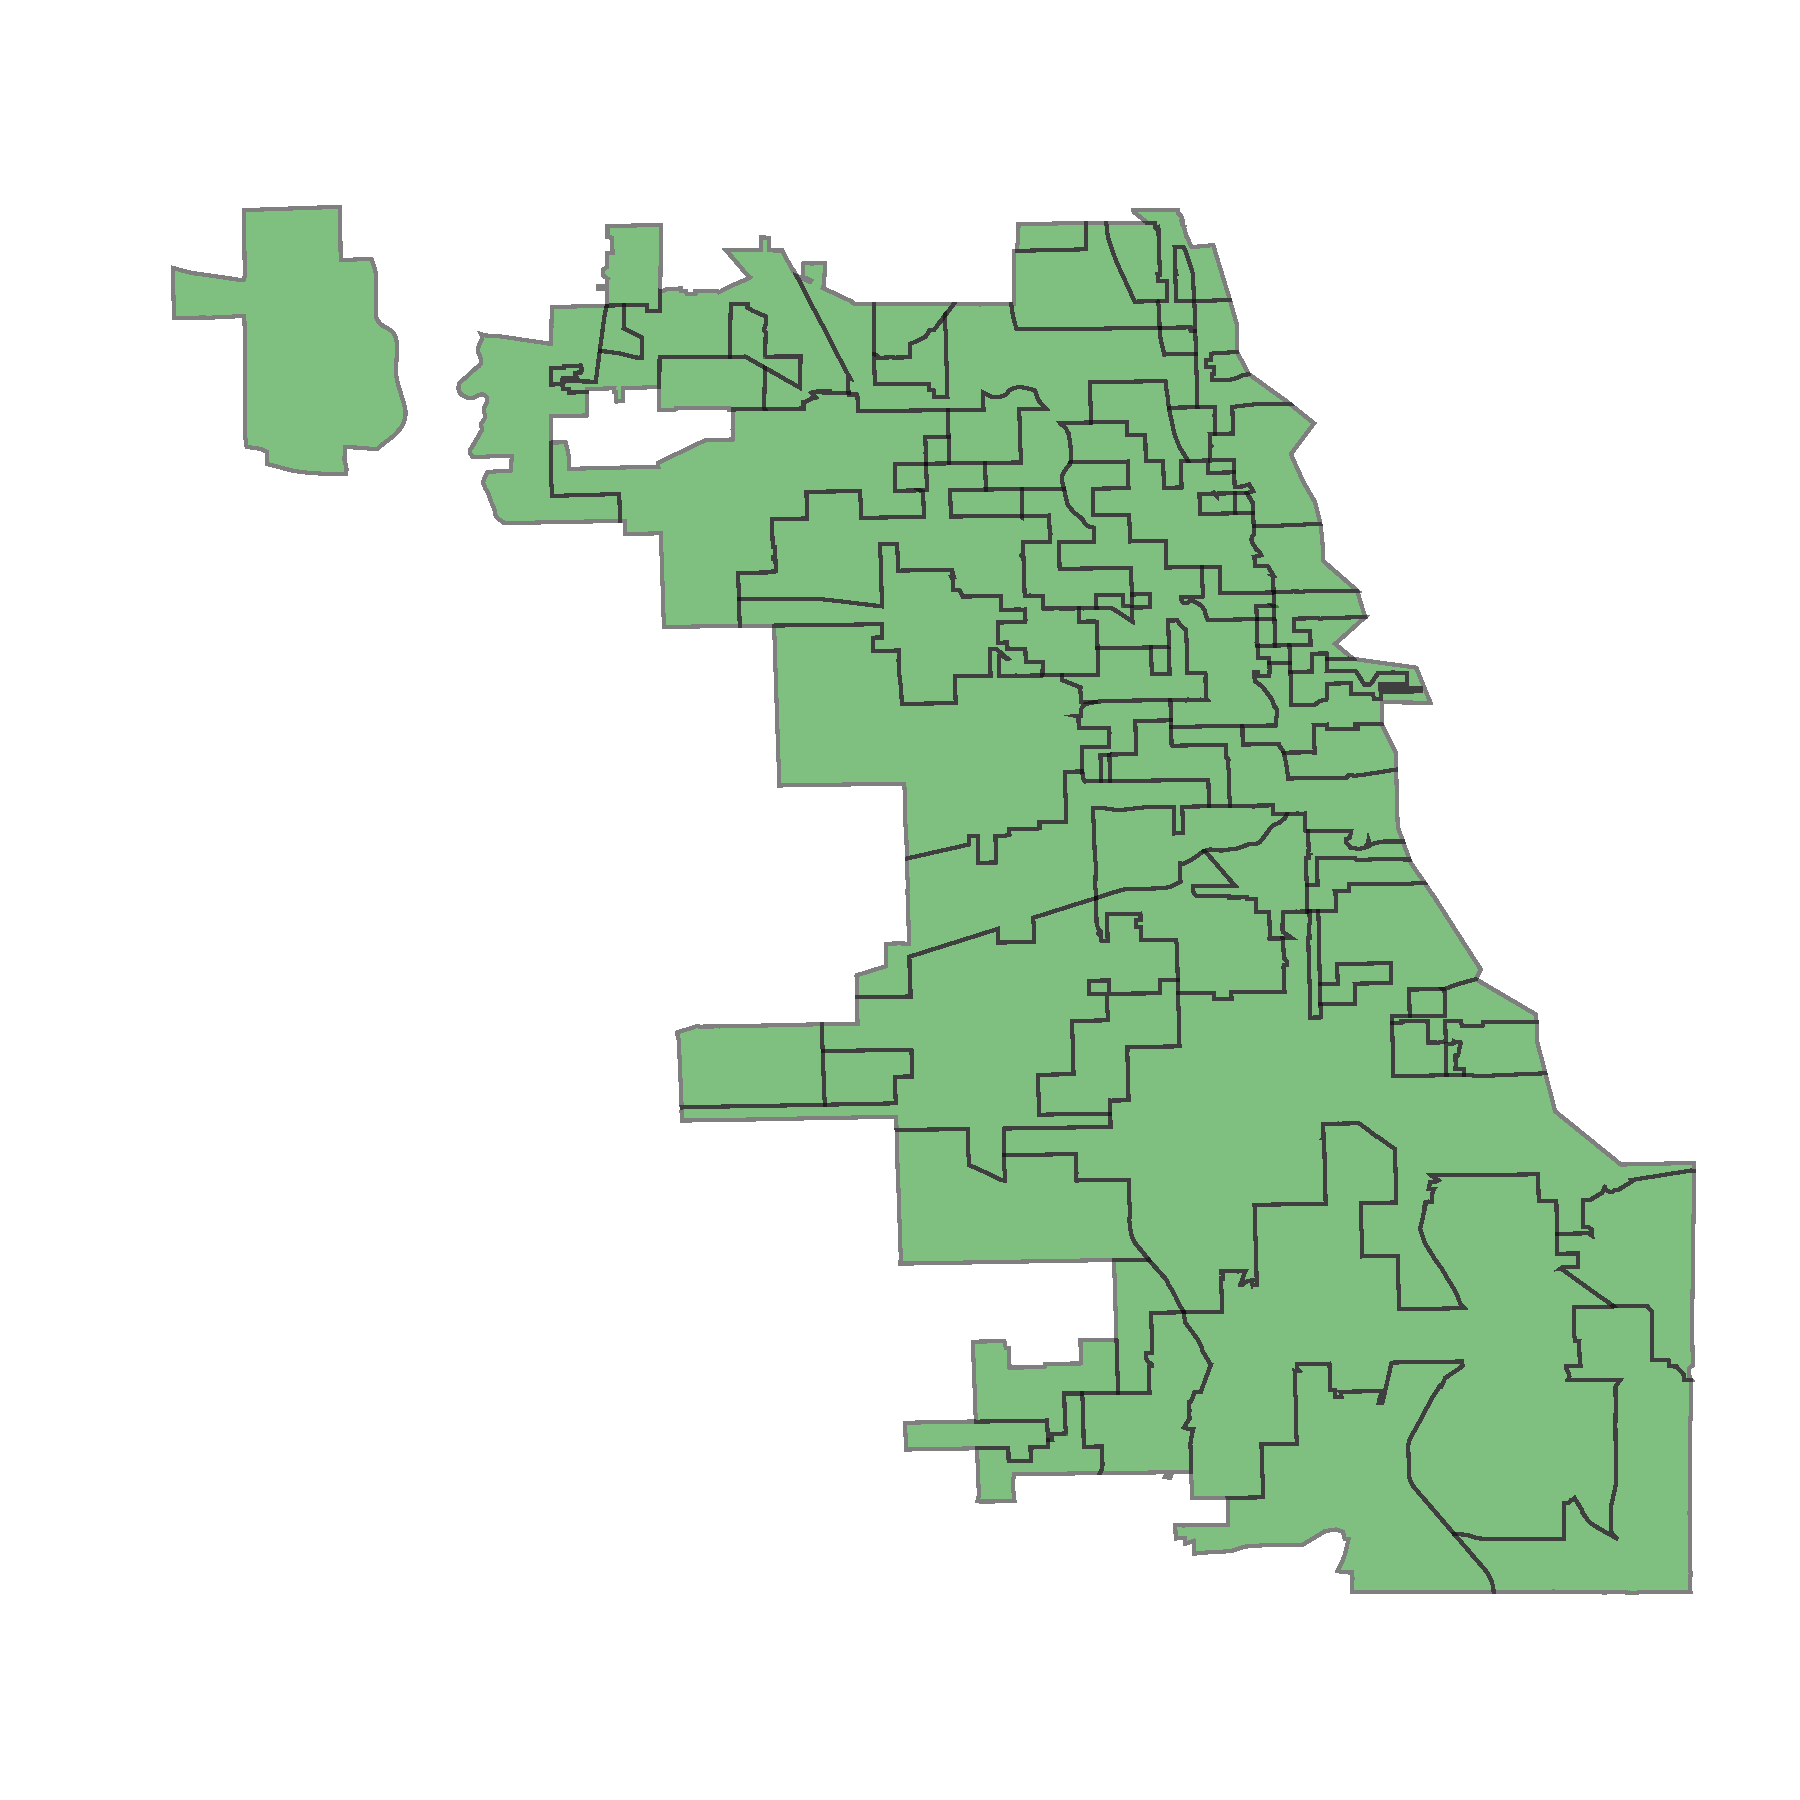
\includegraphics[width=0.45\linewidth]{fig/agg_CAs.pdf}}
\subfigure[\texttt{K-Means}]{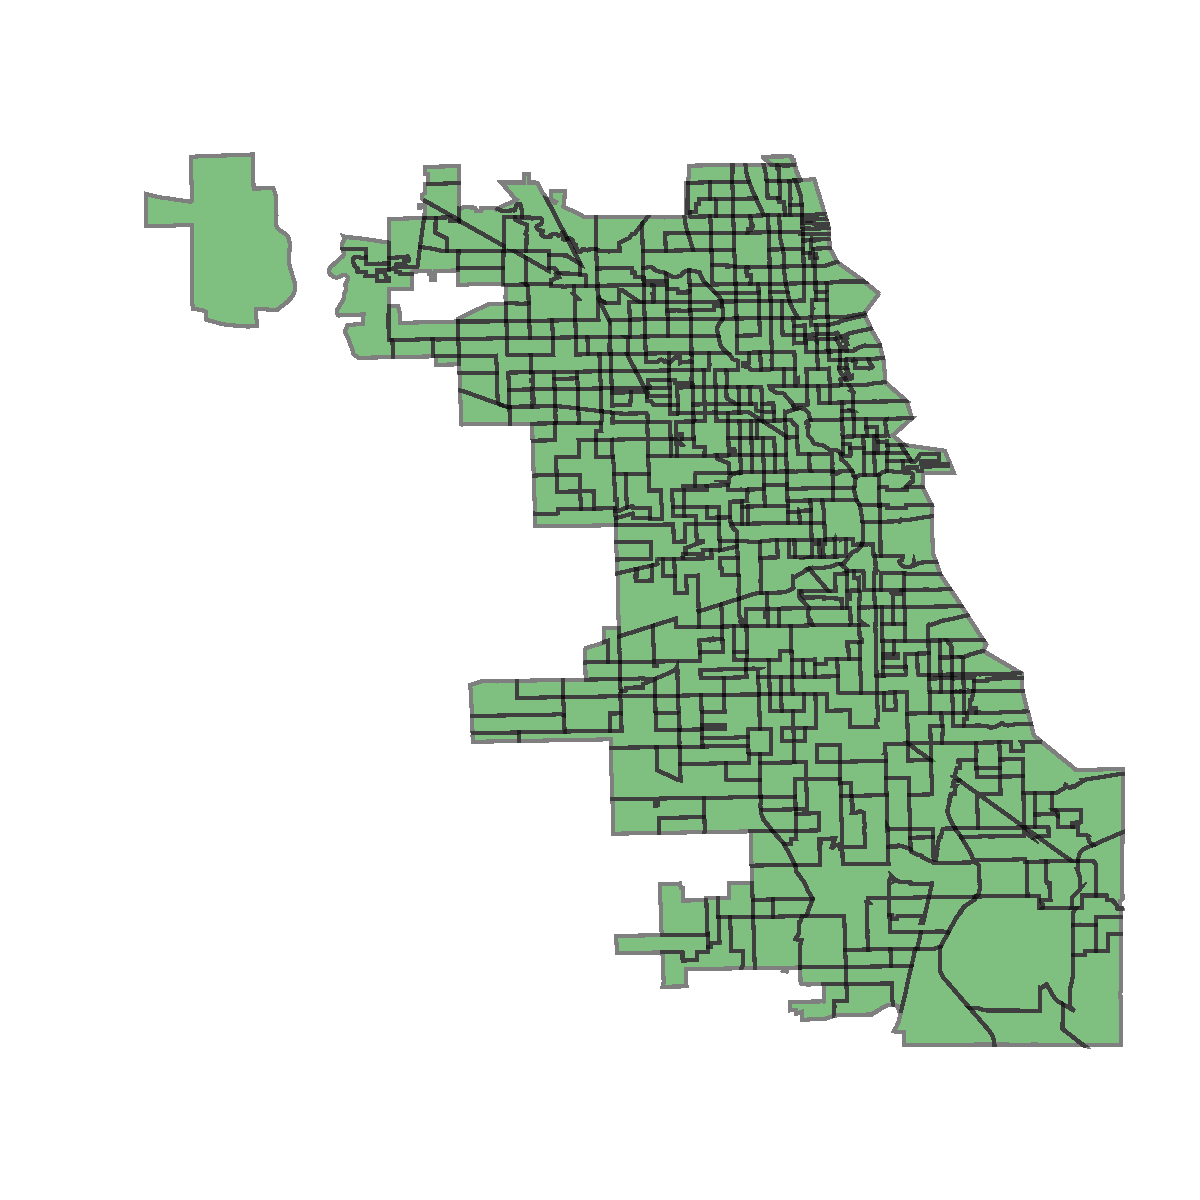
\includegraphics[width=0.45\linewidth]{fig/kmeans_CAs.pdf}}
\subfigure[\texttt{Spectral}]{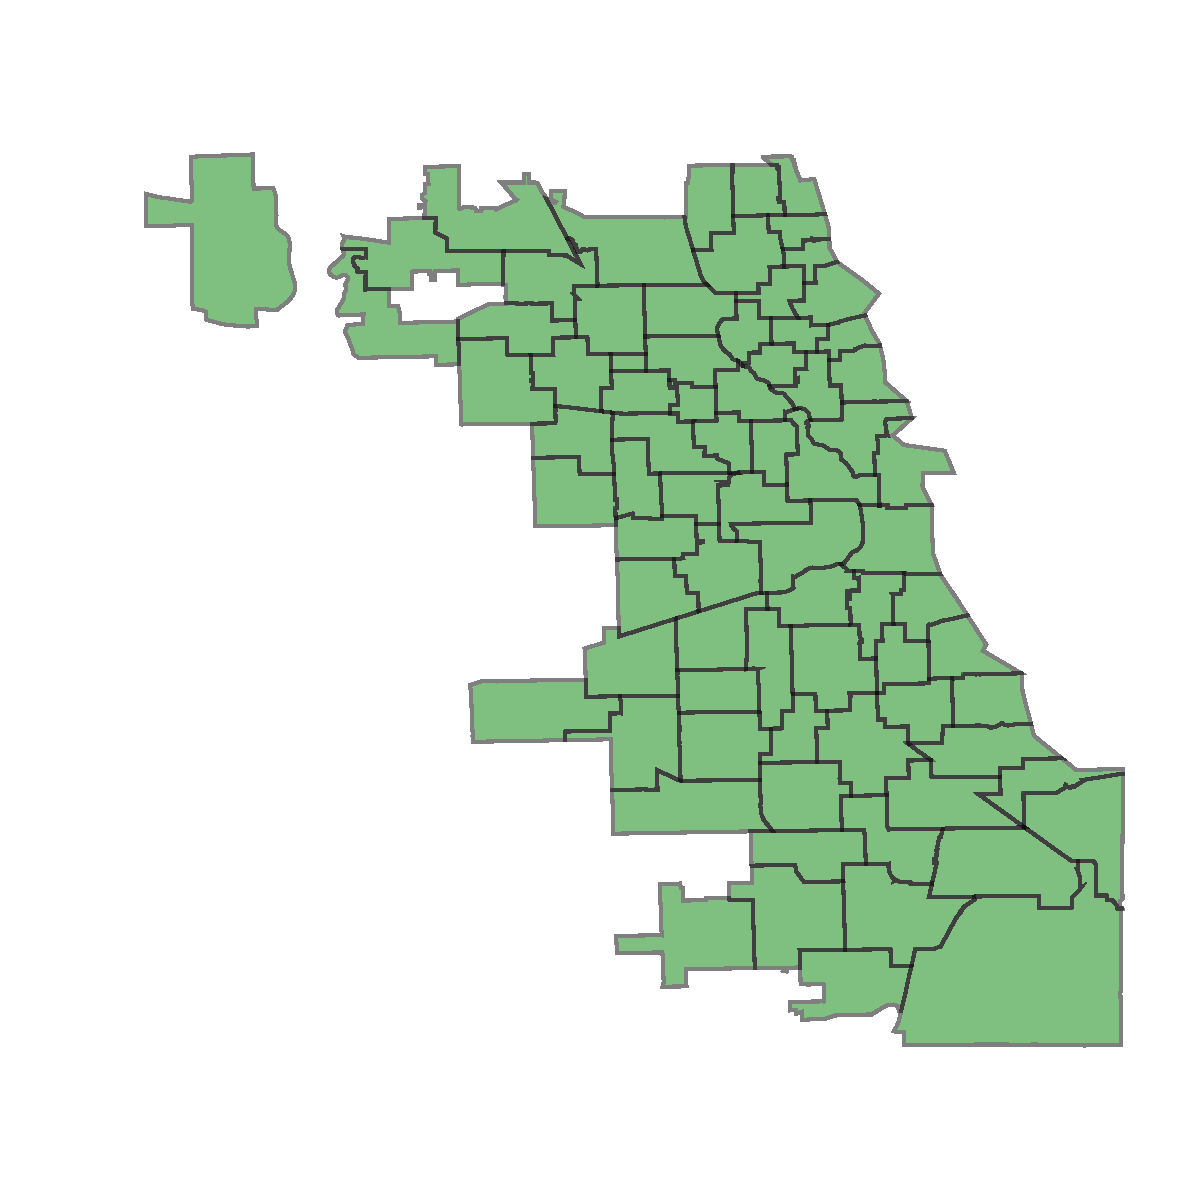
\includegraphics[width=0.45\linewidth]{fig/spectral_CAs.pdf}}
\subfigure[\texttt{DQN}]{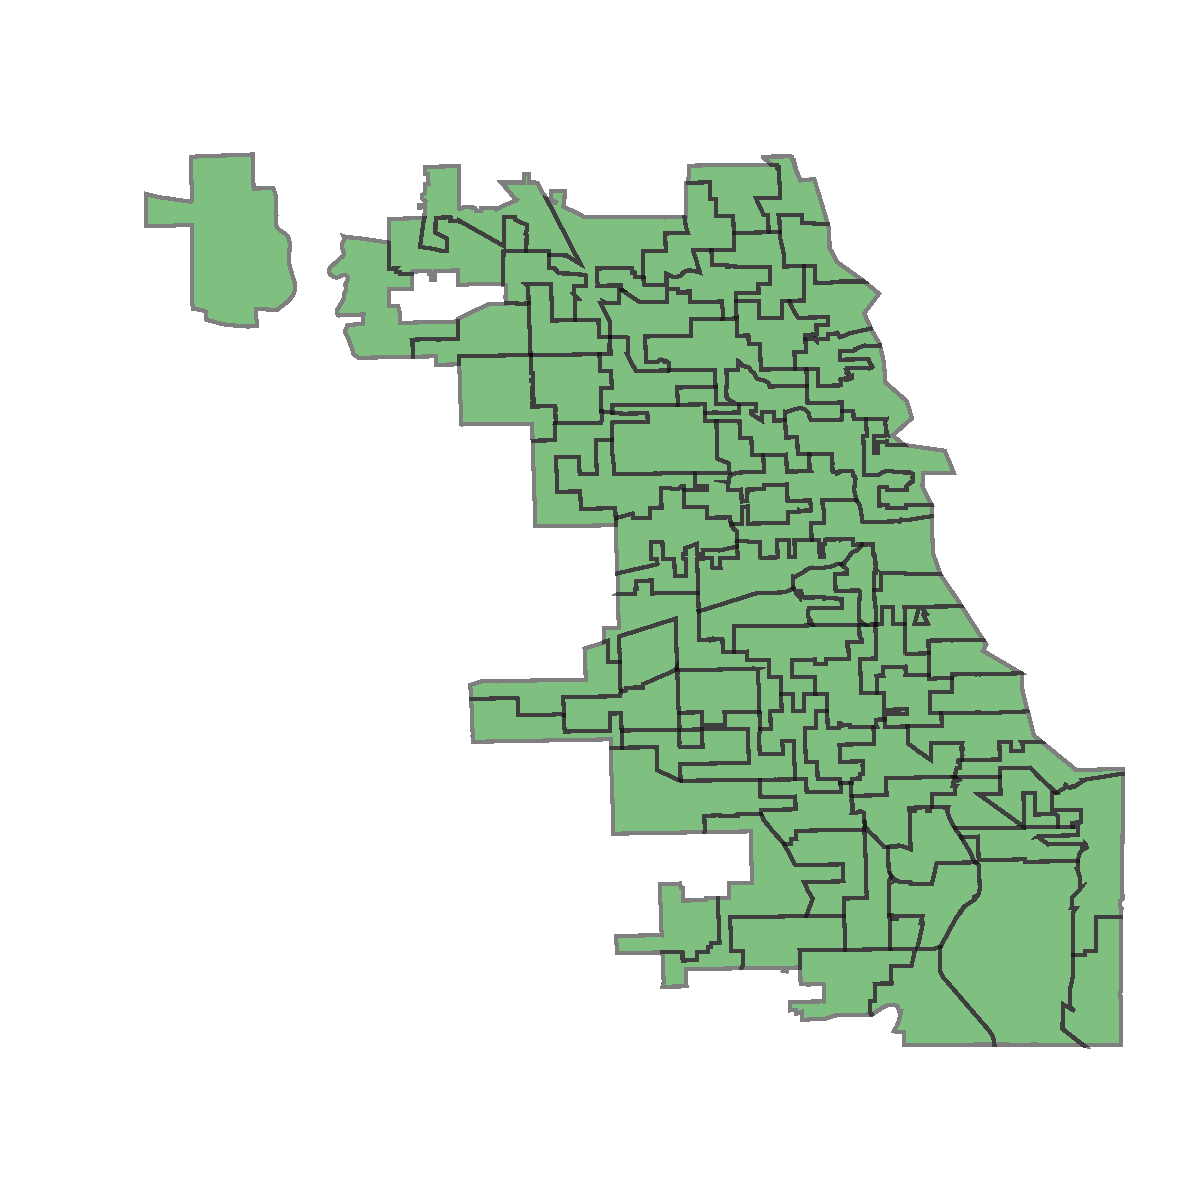
\includegraphics[width=0.45\linewidth]{fig/case-study-house-price-q-learning-v10-CAs.pdf}}
\caption{(a - c) The clustering results for three clustering baselines. (d) The learned partition from \texttt{DQN} method for crime prediction task.}
\label{fig:partitions}
\end{figure*}



\begin{itemize}[leftmargin=*]
\item \textbf{(\texttt{Admin})} Administrative boundary  uses the existing administrative boundary defined by US Bureau of Census~\cite{census:2010}. A visual depiction of this partition can be seen in Figure~\ref{fig:intro}. %This baseline partition is denoted as \texttt{Admin}. 
\item \textbf{(\texttt{Agglomerative})} Agglomerative clustering performs a hierarchical clustering using a bottom up approach. The ward linkage function is used, along with a tract adjacency graph as input to guarantee spatial continuity. %This method is denoted as \texttt{Agglomerative}.
\item \textbf{(\texttt{K-Means})} K-means clustering separates tracts into $n$ groups of equal variance.%, denoted as \texttt{K-Means}.
\item \textbf{ (\texttt{Spectral})} Spectral clustering does a low-dimensional embedding of the affinity matrix between samples first, and then applies the K-means method in the lower dimensional space. Note that \texttt{Spectral} also takes the tract adjacency graph as the affinity graph.
\item \textbf{(\texttt{Naive})} MCMC with naive proposal. The first variant of our proposed MCMC method using a straightforward uniform proposal.
\item \textbf{(\texttt{Softmax})} MCMC with softmax proposal is another variant of our MCMC method, which uses strong heuristics.
\item \textbf{(\texttt{DQN})} Q-learning is our proposed reinforcement learning method to search for optimal partition.
\end{itemize}

For various clustering methods, we set the number of clusters as $m=77$, which equals the number of community areas in \texttt{Admin}. Note that if we run clustering methods multiple times, they usually produce the exact same clustering results. The MCMC and \texttt{DQN} methods, on the other hand, are all stochastic processes and do not converge to the same partition. Therefore, we run $100$ rounds of our proposed methods and report the average measure.



\subsubsection{Evaluation Metrics} 


Given a partition $\mathcal{Z}$, we evaluate the quality of this partition on the testing data set.
Mean absolute error (MAE) is used to measure the performance of prediction tasks, i.e.
\begin{equation}
MAE = \frac{ \sum_{j=1}^m |Y_j - \hat{Y_j}| }{ m},
\end{equation}
where $\hat{Y_i}$ is the leave-one-out prediction error of community $Z_j$. Namely, we train a model on the rest of the communities $\mathcal{Z} \setminus Z_j$. Then, $\hat{Y_j}$ is the estimated target value for $Z_j$ from the trained model.


\subsection{Quantitative Evaluations}

\subsubsection{Effectiveness Study}

In Table~\ref{tab:mae}, we report the evaluation results of the various partition methods. The partitions results from different baselines are visualized in Figure~\ref{fig:partitions}(a-c). Since our methods are run for 100 rounds, we report both the MAE and its standard deviation in the table. The final partition of \texttt{DQN} is visualized in Figure~\ref{fig:partitions}(d). Overall, we have the following three observations.


\begin{table}[h!]
\centering
\caption{Prediction MAEs of various partition methods. Our proposed methods are run for 100 rounds. The MAE and its variance are reported.}
\label{tab:mae}
\begin{tabular}{ |c|>{\raggedleft\arraybackslash}p{4cm}|>{\raggedleft\arraybackslash}p{4cm}|} 
\hline
 Method & \multicolumn{2}{c|}{MAE}  \\ \hline
   & Crime & House price \\
 \hline
 \texttt{Admin} & 1715.91 & 31.29  \\ 
 \hline
 \texttt{Agglomerative} & 72201.00 & 50.34 \\
 \hline
 \texttt{K-means} & 2887.83 & 32.40 \\
 \hline
 \texttt{Spectral} & 1440.57 & 29.66  \\
 \hline
 \texttt{Naive} & 1073.42(81.93) & 25.73(2.76) \\
 \hline
 \texttt{Softmax} & 1041.68(76.75) & 27.13(2.98) \\
 \hline
 \texttt{DQN} & \textbf{746.13}(154.19) & \textbf{25.16}(1.30) \\
 \hline
\end{tabular}
\end{table}


\emph{Clustering methods overall perform poorly}. This is likely due to the fact that the clustering methods do not consider the task information. More specifically, \texttt{Agglomerative} results in the highest prediction errors for both crime prediction and house price prediction task. The reason is that  \texttt{Agglomerative} method utilizes tract connectivity as a hard constraint. As a result, the generated communities have a large variance in their sizes, as shown in Figure~\ref{fig:partitions}(a).  \texttt{K-Means} gives worse result than that of \texttt{Admin} as well. The generated partition of \texttt{K-Means} seems to consist of more than $m$ communities in Figure~\ref{fig:partitions}(b) because \texttt{K-Means} does not incorporate spatial continuity constraint. Consequently, one community can consist of several disconnected components.  \texttt{Spectral} methods generates the best results in both tasks among these baselines because \texttt{Spectral} accounts for the affinity of tracts and generates communities with similar sizes. However, it is worth mentioning that  \texttt{Spectral} method cannot guarantee the spatial continuity of generated communities. From Figure~\ref{fig:partitions}(c), we can also see that \texttt{Spectral} shows similar partition as the original administrative boundary, shown in Figure~\ref{fig:intro}(a). That is also why it achieves similar prediction accuracy as \texttt{Admin}.



\emph{The proposed MCMC method outperforms the baselines}. Both variants of MCMC methods significantly outperform  \texttt{Admin} and \texttt{Spectral} baselines. Such observations validate the effectiveness of the MCMC strategy in searching for optimal solutions. However, it is not conclusive to say \texttt{Softmax} is better than \texttt{Naive}, because while \texttt{Softmax} has better performance on crime prediction task,  \texttt{Naive} has better performance in house price prediction. The reason could be that the heuristics used in \texttt{Softmax} is not universally applicable. The heuristic assumes that working on a community with the highest error will lead to optimal solution. When this heuristic is wrong, it aggressively reduces the search space, excluding where there are better local optimal partitions. 



\emph{ \texttt{DQN} method performs the best among all}. It is clear that  \texttt{DQN} finds a better local optimal solution than that of MCMC methods. On the crime prediction task, the average MAE is $746.13$, which represents a $56\%$ improvement over  \texttt{Admin} baseline. On the house price prediction task, \texttt{DQN} consistently gives the best performance. The reason is that \texttt{DQN} explores over a subset of actions and picks the best one at each step, compared to the MCMC method, which searches the partition space in a depth first search fashion. Comparing the final partition of \texttt{DQN} and \texttt{Spectral}, we will notice that \texttt{Spectral} partition is more similar to the original administrative boundary in Figure~\ref{fig:intro}. As a consequence,  \texttt{Spectral} has similar MAE to \texttt{Admin}, but is much worse than \texttt{DQN}.


\begin{figure}[t!]
\centering
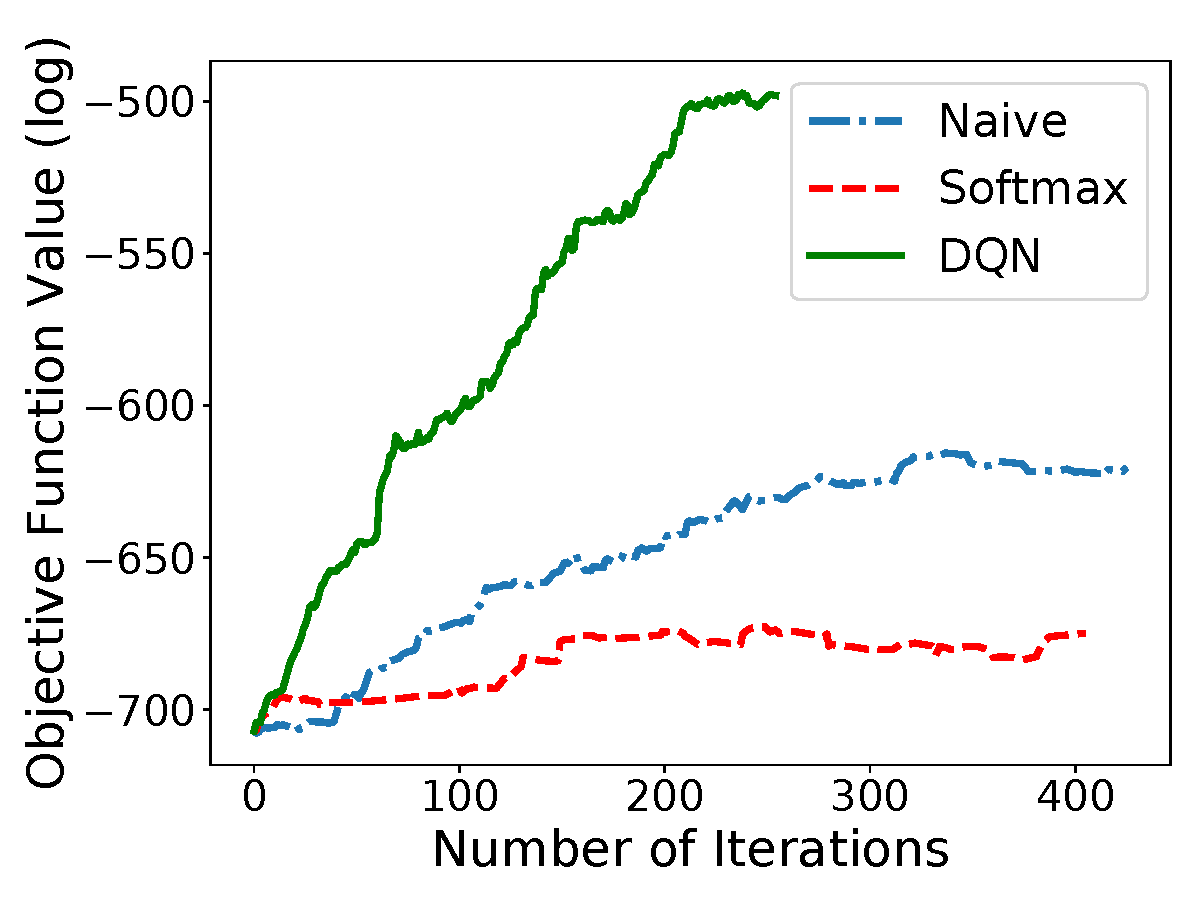
\includegraphics[width=0.9\linewidth]{fig/convergence-study.pdf}
\caption{Convergence plots for proposed methods on house price prediction task.}
\label{fig:convergence}
\end{figure}



\begin{figure*}[t!]
\centering
\subfigure[All communities]{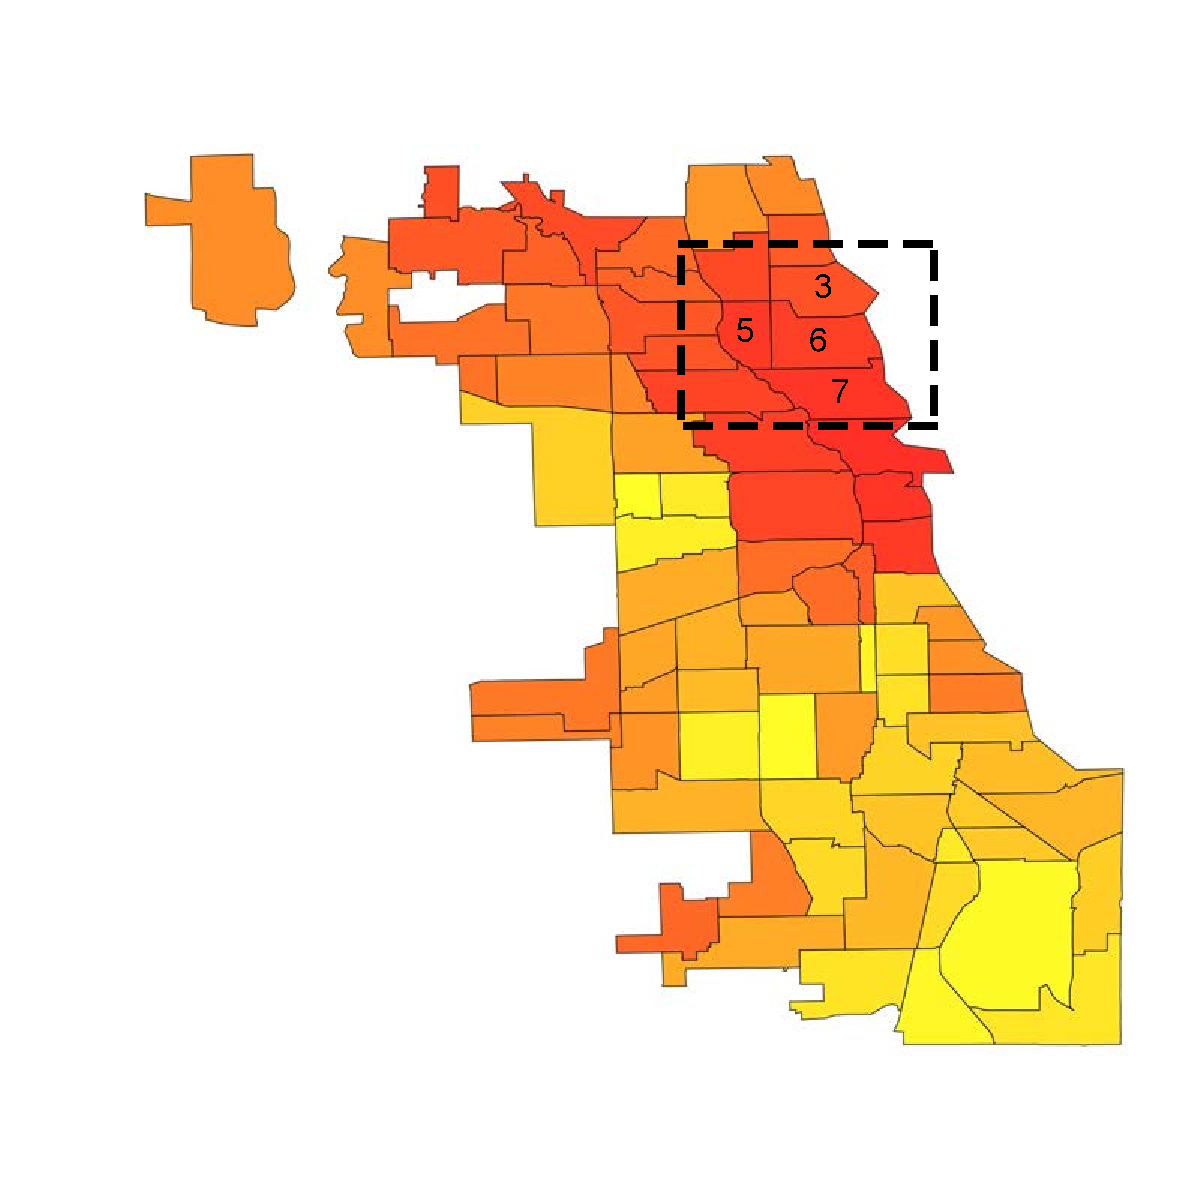
\includegraphics[width=0.3\linewidth]{fig/before-train_average_house_price-all-final.pdf}}
\subfigure[Before]{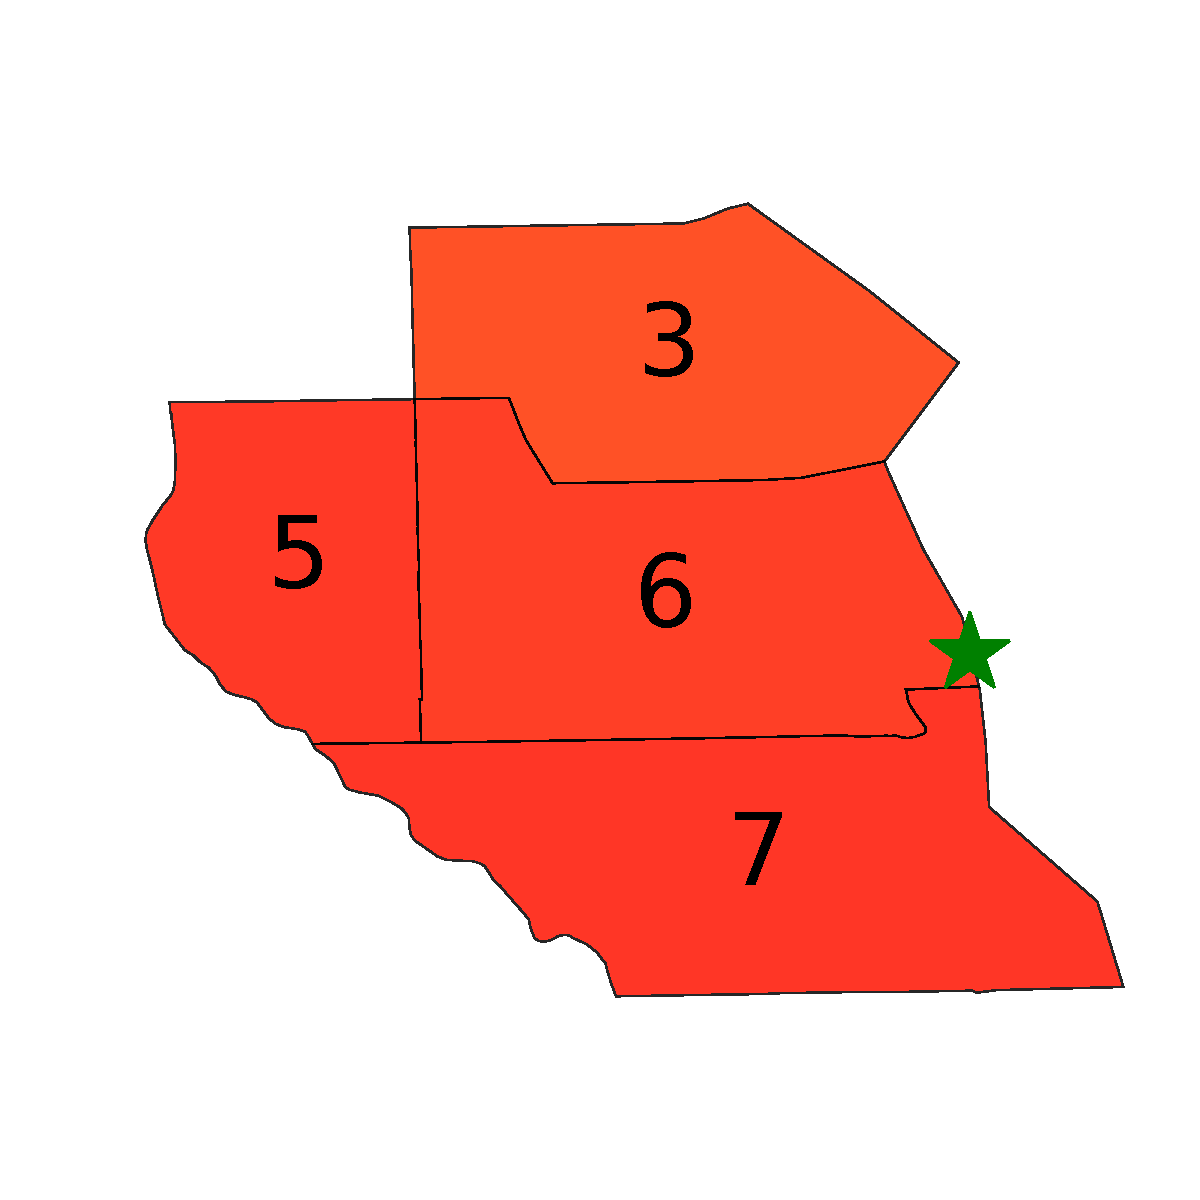
\includegraphics[width=0.28\linewidth]{fig/before-train_average_house_price.pdf}}
\subfigure[After]{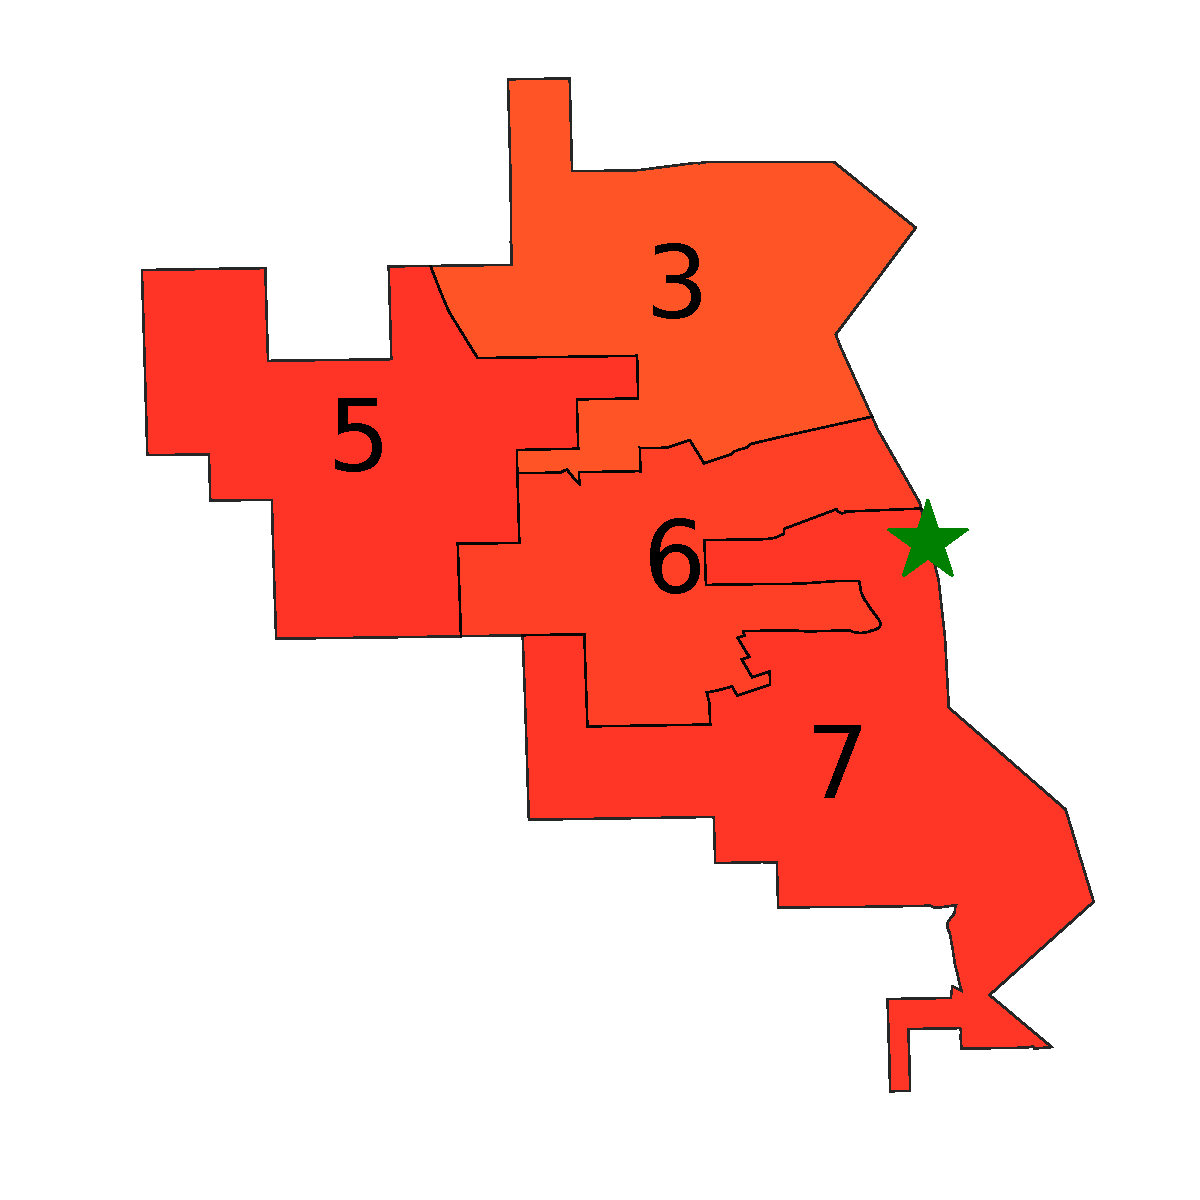
\includegraphics[width=0.3\linewidth]{fig/after-train_average_house_price.pdf}}
\subfigure[Lake View]{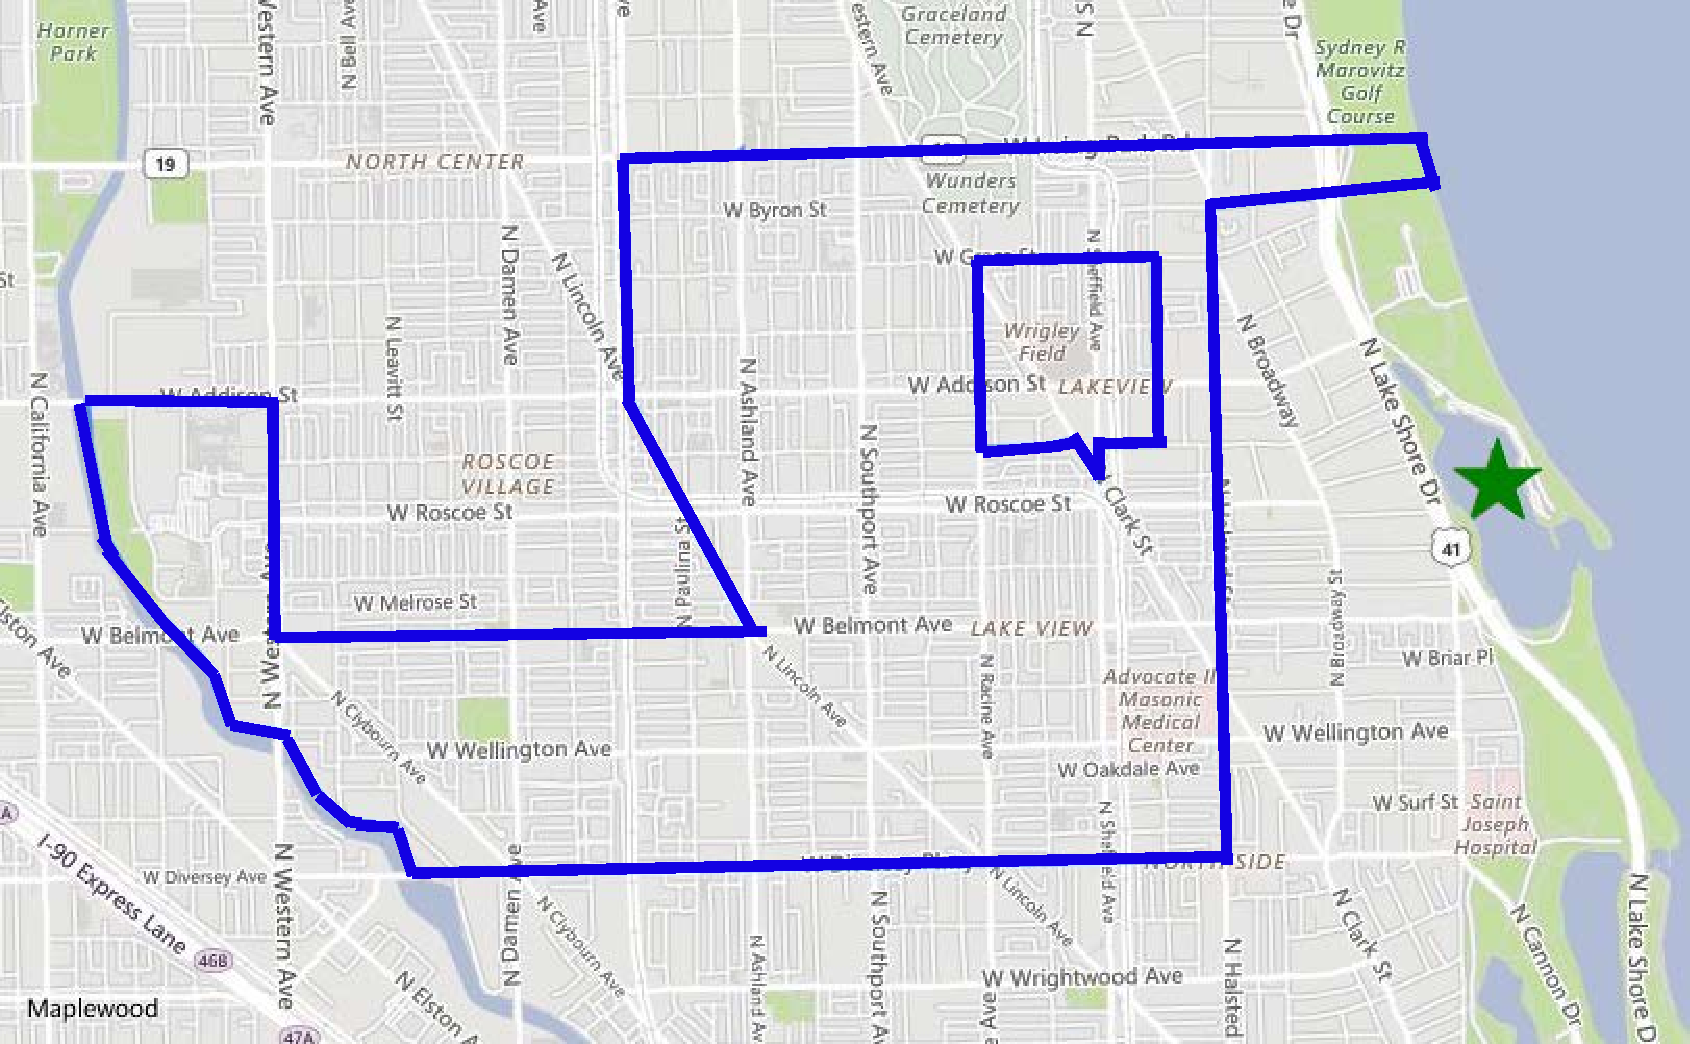
\includegraphics[width=0.45\linewidth]{fig/ca-lakeview.pdf}}
\subfigure[Lake View East]{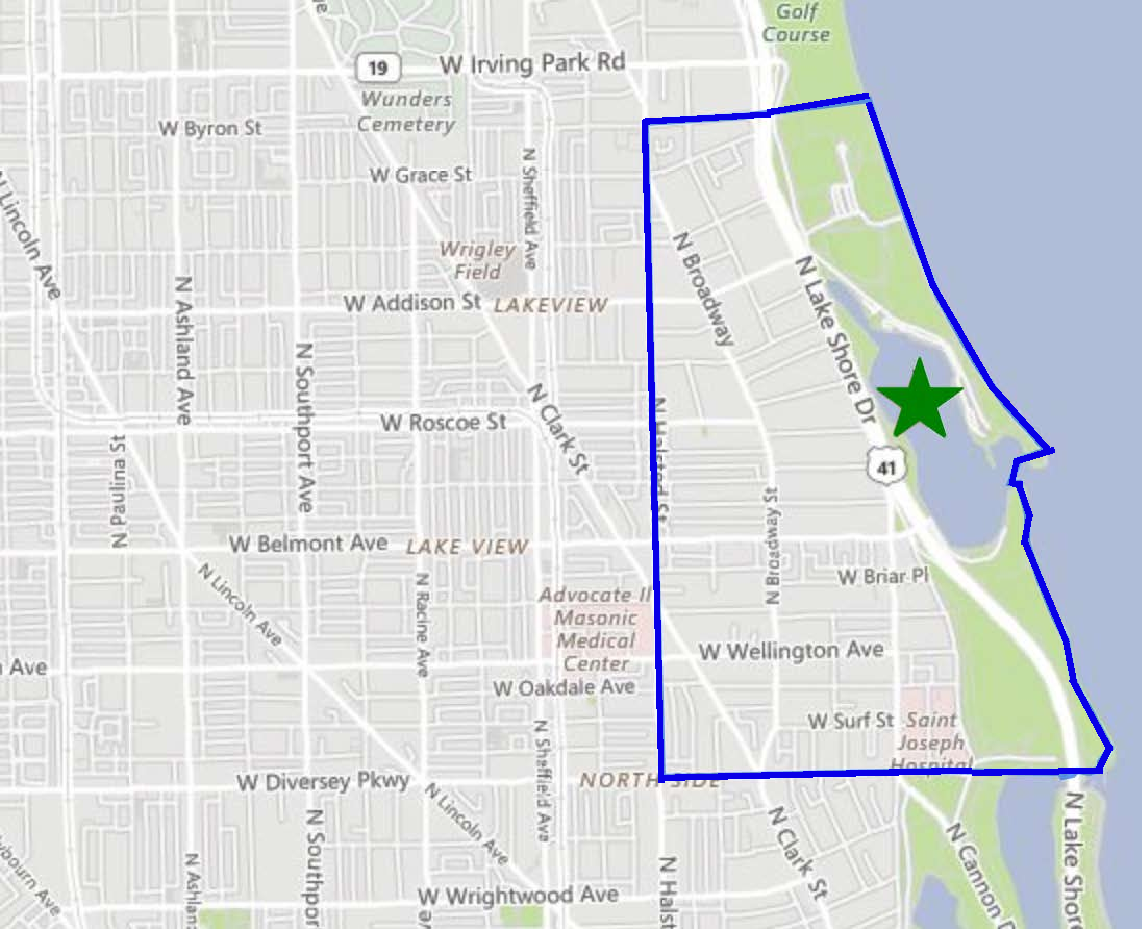
\includegraphics[width=0.34\linewidth]{fig/ca-lakeview-east.pdf}}
\caption{House price prediction case near Belmont Harbor, denoted by green star. (a) Average house price distribution in Chicago under \texttt{Admin} partition. Dotted rectangle denotes region of interest. (b) Region of interest under \texttt{Admin} partition. (c) Region of interest under \texttt{DQN} partition. (d - e) Region of interest according to Zillow. Note that the Belmont Harbor area is split into a separate community, named Lake View East.}
\label{fig:housePrice}
\end{figure*}



\subsubsection{Convergence Study}

We conclude the effectiveness study with a brief comparison of the convergence of three proposed methods. In our method, we track the standard deviation of the $\mathcal{F}$ values from last $50$ iterations. When such standard deviation is less than a pre-defined threshold, we stop. In Figure~\ref{fig:convergence} we visualize log of quality measure, i.e. $ - \mathcal{F}(\mathcal{Z})$, against the number of iterations for three proposed methods on the house price task. 

We observe that \texttt{DQN} finishes in a less than 300 iterations, while \texttt{Naive} and \texttt{Softmax} both take more than 400 iterations. Clearly, we observe that \texttt{DQN} converge to a better optimal solution with higher training gain. Comparing with \texttt{Naive},  \texttt{Softmax} converges faster at the beginning, because of the strong heuristics behind. However, \texttt{Naive} eventually finds a better local optimal solution than that of \texttt{Softmax}, because the heuristics eliminates search space too aggressively, such that the algorithm could not explore search space with better local optimal partitions.









\subsection{Case Studies}

In this section, we present two interesting case studies of the region partitions learned from \texttt{DQN} method.

\smallskip
\textbf{House price prediction case study}. We present a case study near community \#6, Lake View, in the house price prediction task, as shown in Figure~\ref{fig:housePrice}. This case shows that \texttt{DQN} partition is actually superior to the original administrative boundary, because  \texttt{DQN} partition matches better with expert domain knowledge.

We visualize a heat map of house price (per square foot) for the whole city of Chicago in Figure~\ref{fig:housePrice}(a). Warmer colors (red) denote higher prices, while cooler colors (yellow) indicate lower prices. The dotted rectangle in the figure marks the region of interest for our discussion, which is community \#6. A zoom-in view of this area using the administrative boundary is shown in Figure~\ref{fig:housePrice}(b). Notice that all nearby areas have relatively high average house price.


Recall from the Figure~\ref{fig:intro-explain} that east side of community \#6 is different from the rest area of community \#6. We further find the following evidence to support the fact that the east side of community \#6 is different from the rest area. The coastal region of the original community \#6 contains Belmont Harbor, one of Chicago's largest boating areas. Notice that  \texttt{DQN} method divides community area \#6 and groups the coastal tracts surrounding the Belmont Harbor with other coastal areas farther south in community \#7. These areas contain other leisure destinations such as the Lincoln Park Zoo, and numerous beach areas. This semantic argument is bolstered by an independent source: Zillow's own self-defined regions. Figure~\ref{fig:housePrice}(d) shows that the Lake View area does not contain Belmont Harbor. Meanwhile, Zillow assigns Belmont Harbor as a separate region called Lake View East, as shown in Figure~\ref{fig:housePrice}(e). 


Surprisingly,  \texttt{DQN} partition is similar to Zillow's self-defined region in that they both exclude the Belmont Harbor area from the original community \#6 (Lake View neighborhood), as shown in Figure~\ref{fig:housePrice}(c). While the two regions are not exactly the same, it is interesting to note that they both remove the Belmont Harbor area from the original community.



\begin{figure*}[t!]
\centering
\subfigure[All communities]{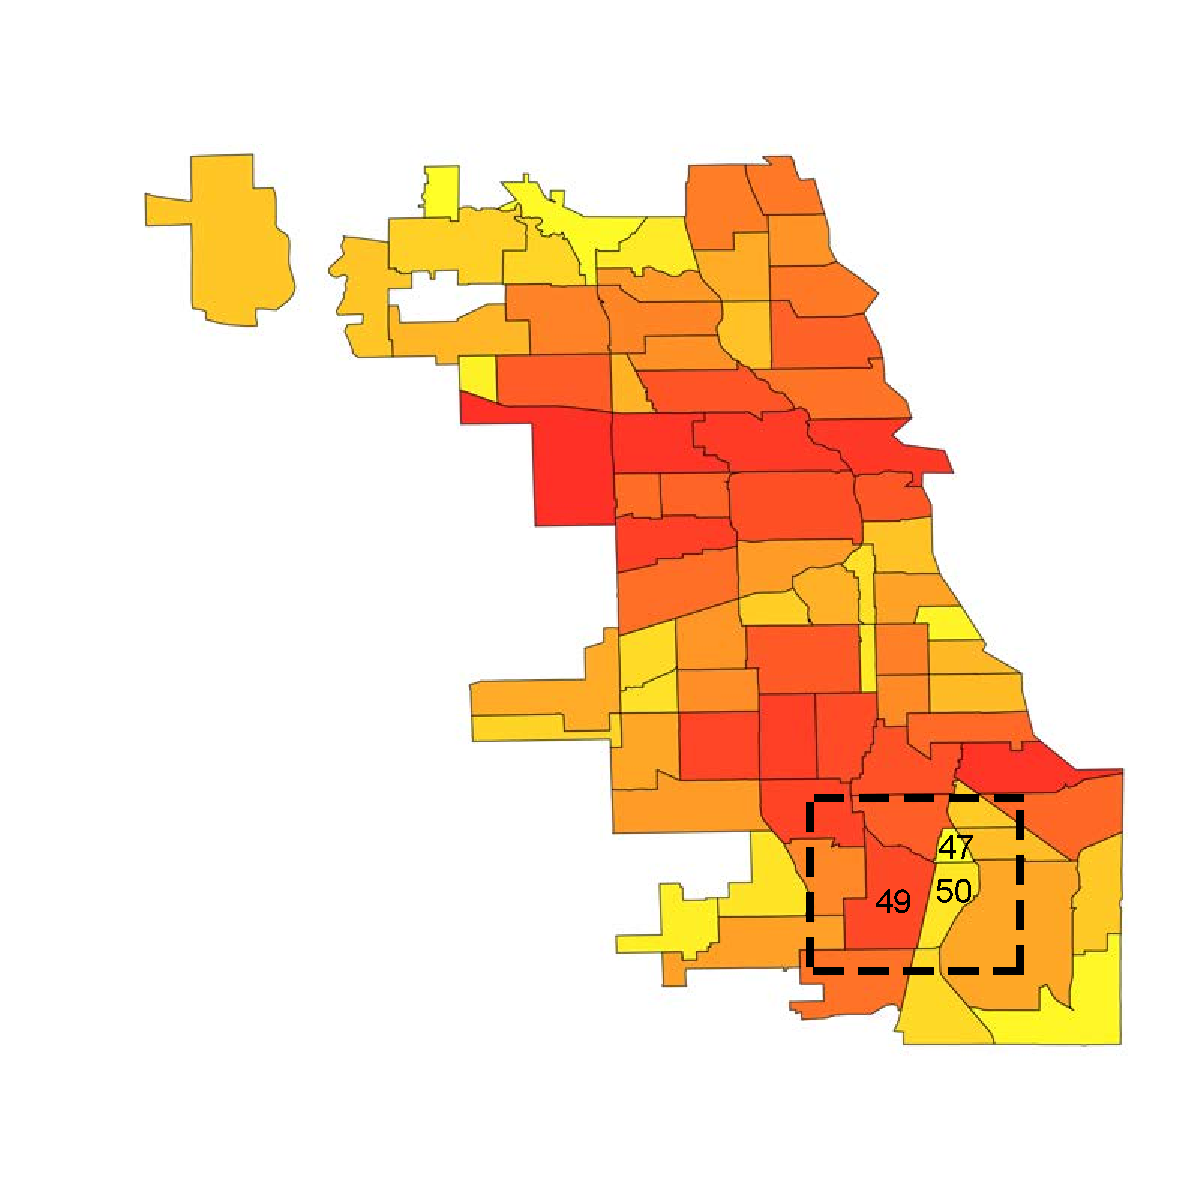
\includegraphics[width=0.3\linewidth]{fig/before-total-all-final.pdf}}
\subfigure[Crime Before]{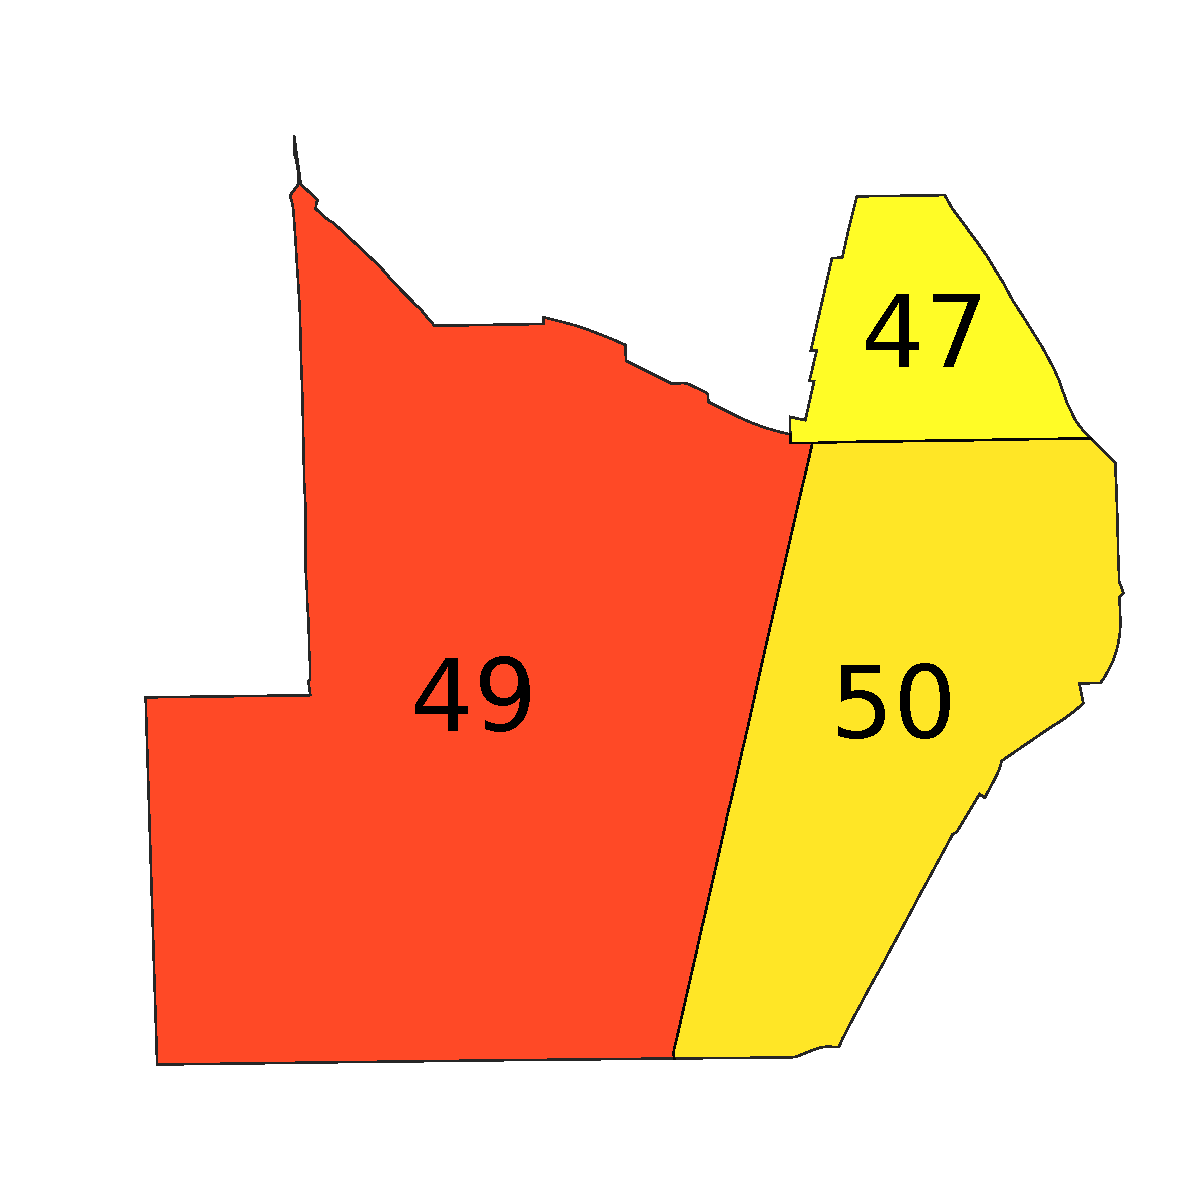
\includegraphics[width=0.28\linewidth]{fig/before-total.pdf}}
\subfigure[Poverty Before]{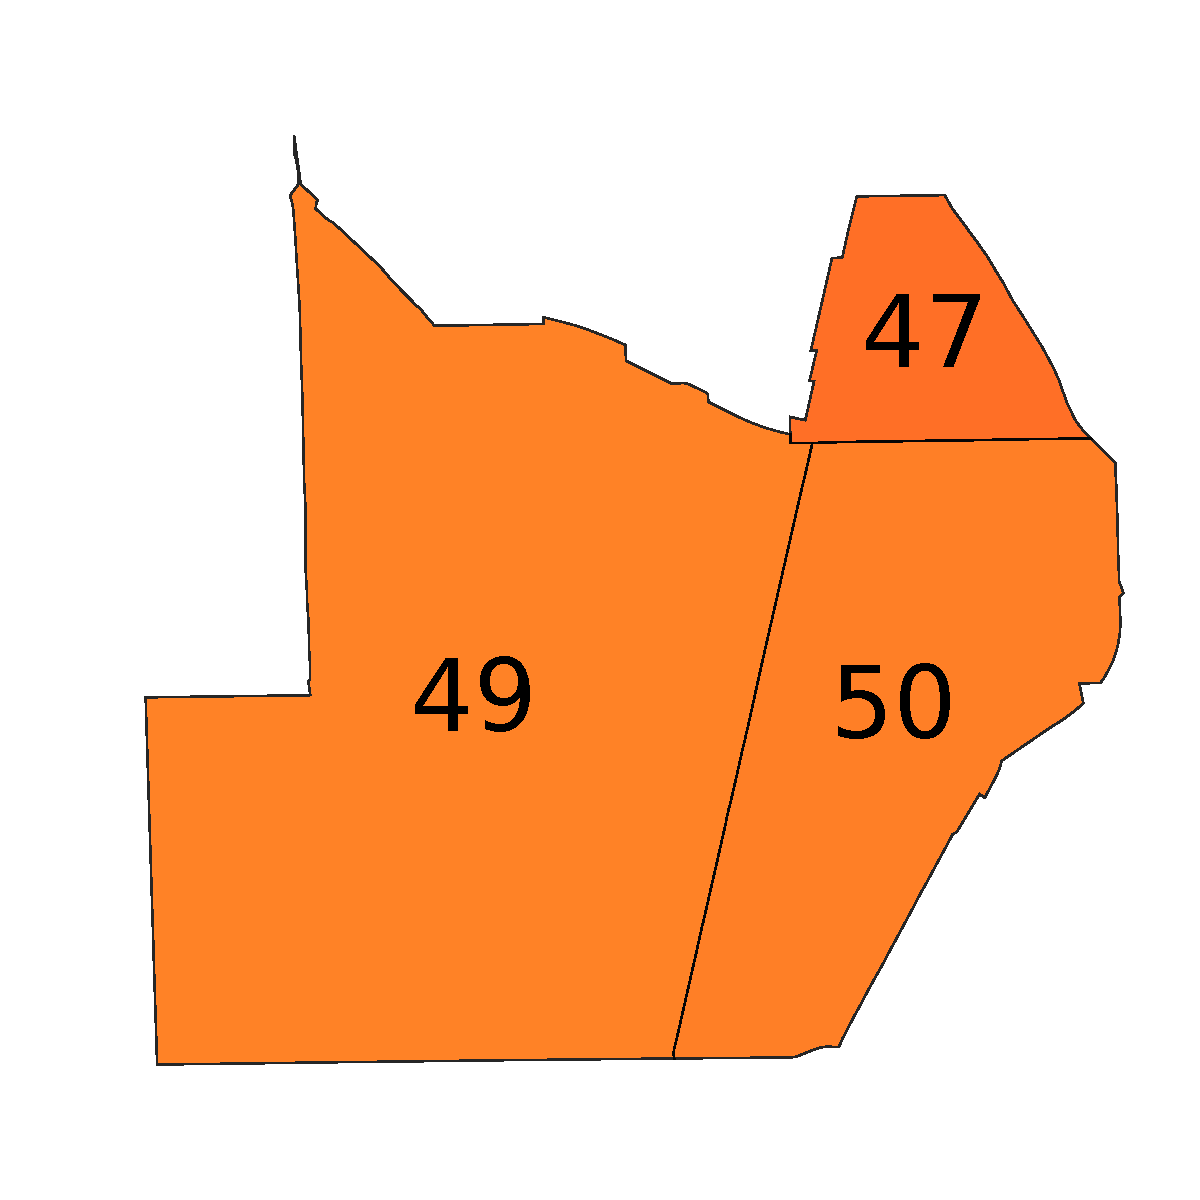
\includegraphics[width=0.28\linewidth]{fig/before-poverty_index.pdf}}
\subfigure[Crime After]{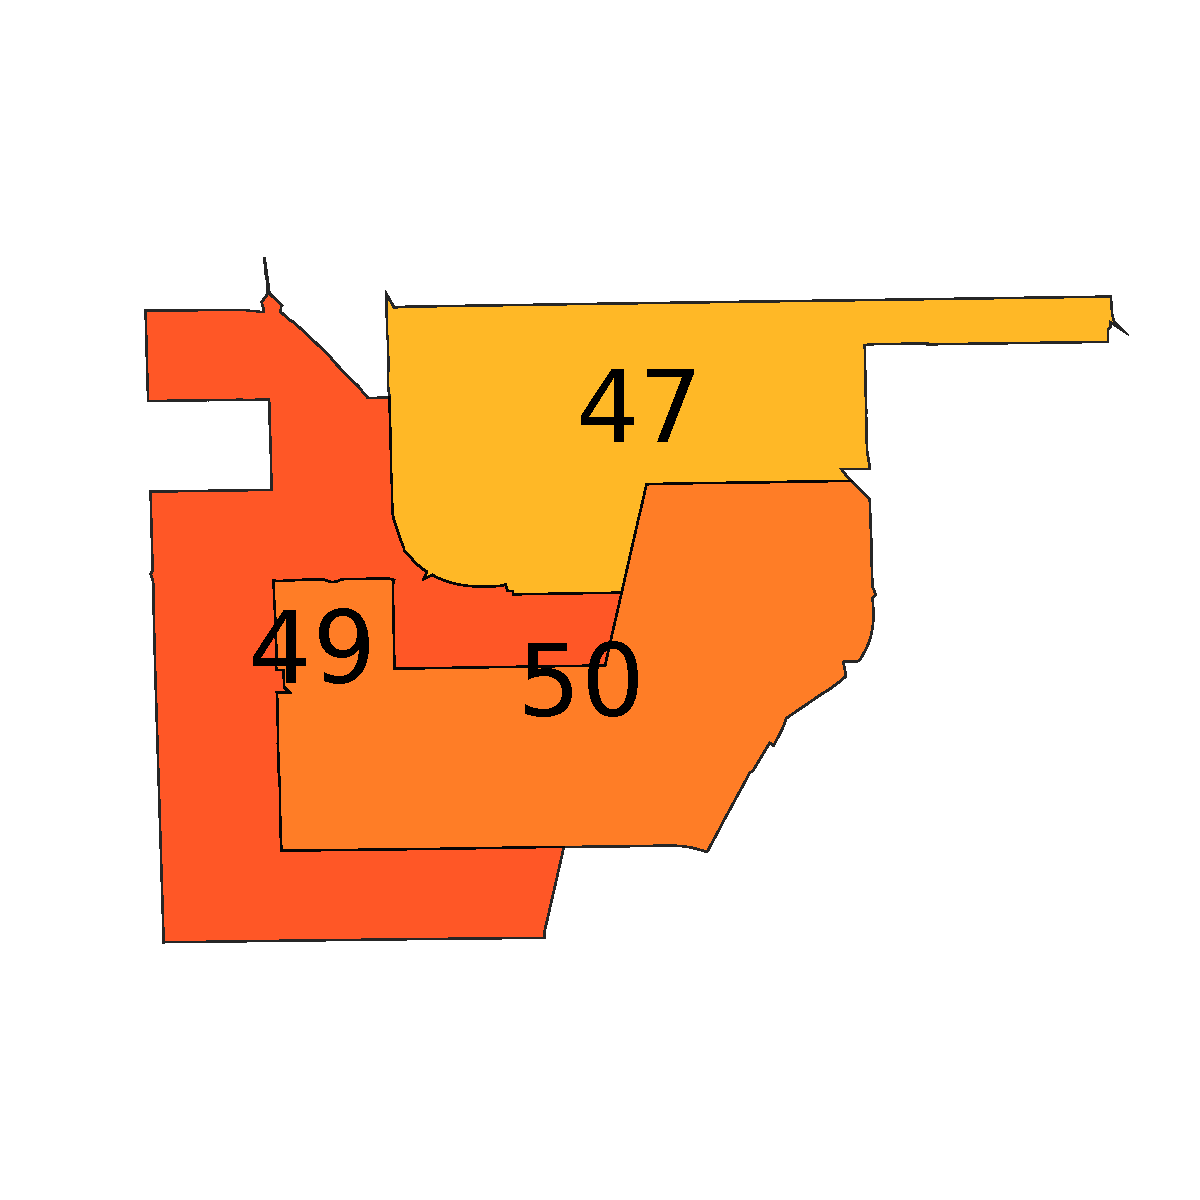
\includegraphics[width=0.32\linewidth]{fig/after-total.pdf}}
\subfigure[Poverty After]{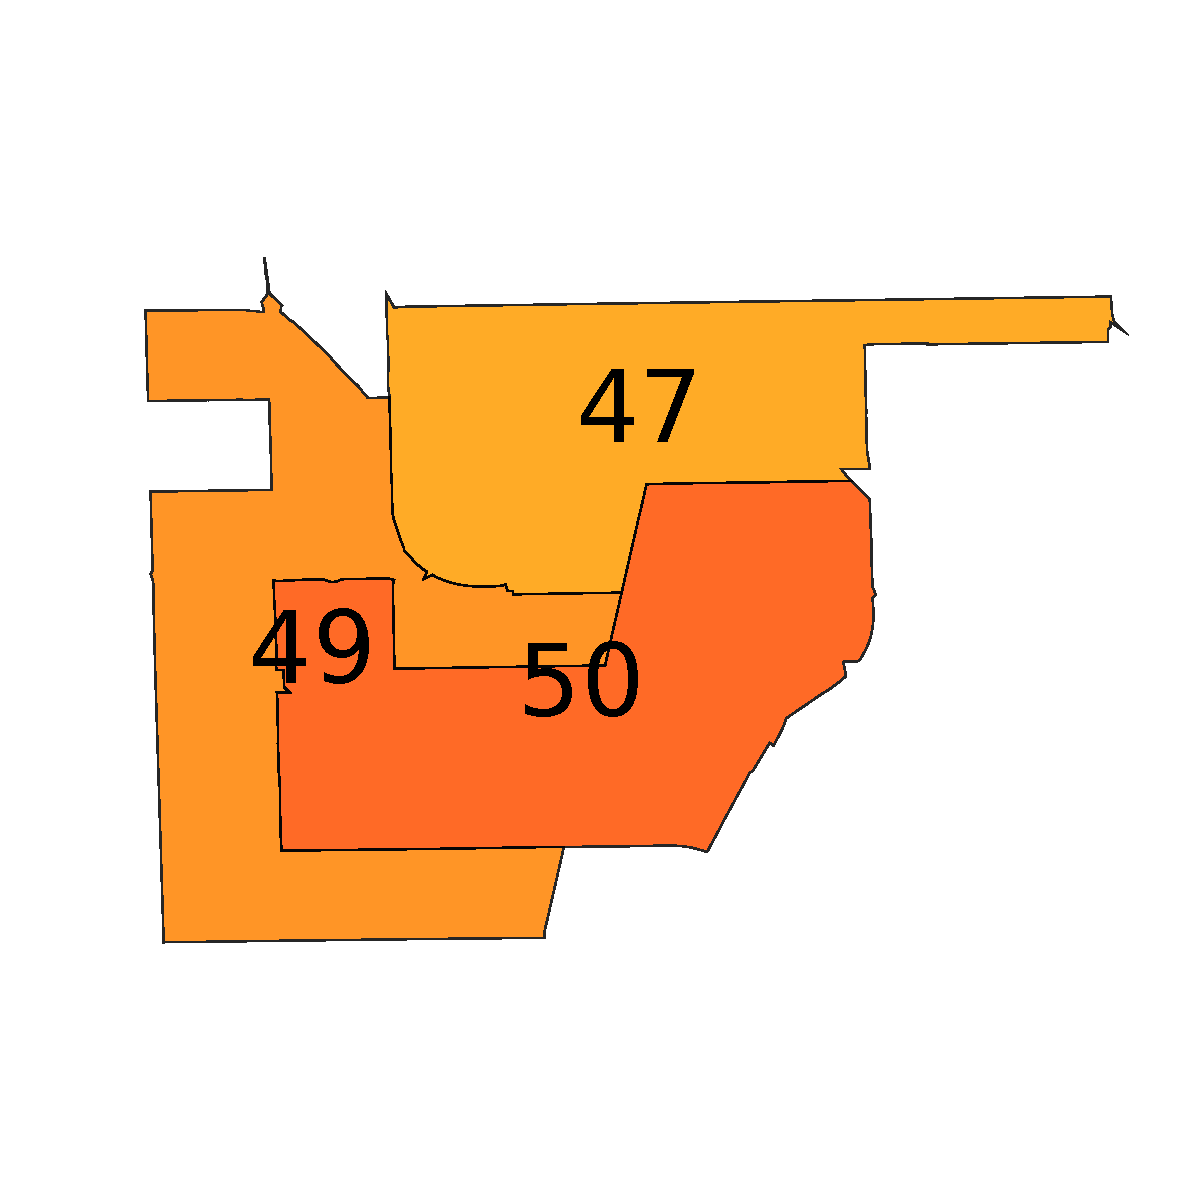
\includegraphics[width=0.32\linewidth]{fig/after-poverty_index.pdf}}
\caption{Crime prediction case near Community \#47. (a) Crime count distribution in Chicago under \texttt{Admin} partition. Dotted rectangle denotes the region of interest. (b) Crime count in region of interest under \texttt{Admin} partition. (c) Poverty index in region of interest under \texttt{Admin} partition. (d) Crime count in region of interest under \texttt{DQN} partition. (e) Poverty index in region of interest under \texttt{DQN} partition.}
\label{fig:crime-case}
\end{figure*}

\smallskip
\textbf{Crime prediction case study}. For crime study, we give the intuition why our partition gives lower prediction errors in the corresponding task. The case is shown in Figure~\ref{fig:crime-case}.

For the purpose of simplicity, we choose a single feature, that reasonably correlates with our variable of interest, namely crime count. The single feature we choose is the poverty index, which is calculated by the percentage of households in a given community whose combined income is less than or equal to \$30, 000. Figure~\ref{fig:crime-case}(a) shows a heat map of crime count by community, using the original administrative boundary. Warmer areas correspond to higher crime counts. We focus on communities \#47, \#49, and \#50, as marked by the dotted rectangle in Figure~\ref{fig:crime-case}(a). 


A zoom-in plot of the crime count by administrative boundary is shown in Figure~\ref{fig:crime-case}(b). Additionally, we construct a similar plot of the poverty index of these three communities, found in Figure~\ref{fig:crime-case}(c). It is clear that under  \texttt{Admin} partition, these communities are nearly identical in poverty index, while their crime counts differ dramatically. Next, we visualize the crime count and poverty index with  \texttt{DQN} partition in Figure~\ref{fig:crime-case}(d) and Figure~\ref{fig:crime-case}(e), respectively. We can see that these three regions of interest still exhibit similar poverty levels, but their crime counts are much closer to each other.


The observation above reveals the intuition of  \texttt{DQN} partition: it attempts to make the spatial distributions of $X$ and $Y$ similar. In other words, this is how  \texttt{DQN} partition reduces the prediction error.

We also note that community \#47 dramatically increased in size under  \texttt{DQN} partition. Community \#47 used to be the smallest community according to the Chicago’s administrative boundary partition, with a population of less than 3,000 people. The variance penalty in our objective function (Equation~\ref{eq:objective}) causes our proposed method to favor regions that are similar in terms of population. It is likely that this community is expanded to yield better correlation between poverty and crime, as well as balance out the population distribution over communities.





\section{Conclusion}
\label{ch4-sec:conclusion}


In this chapter, we proposed a new problem called task-specific region partition. The problem is motivated by the fact that existing administrative boundaries are static regardless of the target variable, and we observed cases where it is necessary to have different partitions for different tasks. The task-specific region partition problem is NP-hard, and hence directly searching for a global optimal is difficult. Three variants of MCMC methods are proposed to solve this combinatorial optimization problem. First, a Naive MCMC that generates the next sample by random sampling. Second, a heuristic-based, Guided MCMC method that prefers to select from community areas with larger errors to generate the next sample. Finally, we employ reinforcement learning to automatically learn a sample strategy. Our methods are evaluated on two prediction tasks, i.e. crime prediction and real estate price prediction. The learned predictions consistently outperform the administrative boundaries in both tasks.

\chapter{Title of the Fifth Chapter}

\section{Introduction}
When in the Course of human events, it becomes necessary for one people  to dissolve the political bands which have connected them with another,  and to assume among the powers of the earth, the separate and equal station  to which the Laws of Nature and of Nature's God entitle them, a decent respect to the opinions of mankind requires that they should declare  the causes which impel them to the separation.

\section{More Declaration}

We hold these truths to be self-evident, that all men are created equal,  that they are endowed by their Creator with certain unalienable Rights,  that among these are Life, Liberty and the pursuit of Happiness. --That to secure these  rights, Governments are instituted among Men, deriving their just powers  from the consent of the governed, --That whenever any Form of Government  becomes destructive of these ends, it is the Right of the People to alter  or to abolish it, and to institute new Government, laying its foundation on  such principles and organizing its powers in such form, as to them shall  seem most likely to effect their Safety and Happiness. Prudence, indeed, will dictate that Governments long established should not  be changed for light and transient causes; and accordingly all experience  hath shewn, that mankind are more disposed to suffer, while evils are  sufferable, than to right themselves by abolishing the forms to which they  are accustomed. But when a long train of abuses and usurpations, pursuing invariably the same  Object evinces a design to reduce them under absolute Despotism, it is their  right, it is their duty, to throw off such Government, and to provide new Guards for their future security. --Such has been the patient sufferance of these Colonies; and such is now the  necessity which constrains them to alter their former Systems of Government.  The history of the present King of Great Britain [George III] is a history  of repeated injuries and usurpations, all having in direct object the  establishment of an absolute Tyranny over these States. To prove this, let Facts be submitted to a candid world.
%%%%%%%%%%%%%%%%%%%%%%%%%%%%%%%%%%%%%%%%%%%%%%%%%%%%%%%%%%%%%%%
% Appendices
%
% Because of a quirk in LaTeX (see p. 48 of The LaTeX
% Companion, 2e), you cannot use \include along with
% \addtocontents if you want things to appear the proper
% sequence.
%%%%%%%%%%%%%%%%%%%%%%%%%%%%%%%%%%%%%%%%%%%%%%%%%%%%%%%%%%%%%%%
\appendix
\titleformat{\chapter}[display]{\fontsize{30}{30}\selectfont\bfseries\sffamily}{Appendix \thechapter\textcolor{gray75}{\raisebox{3pt}{|}}}{0pt}{}{}
% If you have a single appendix, then to prevent LaTeX from
% calling it ``Appendix A'', you should uncomment the following two
% lines that redefine the \thechapter and \thesection:
%\renewcommand\thechapter{}
%\renewcommand\thesection{\arabic{section}}
\Appendix{Title of the First Appendix}

\section{Introduction}
When in the Course of human events, it becomes necessary for one people  to dissolve the political bands which have connected them with another,  and to assume among the powers of the earth, the separate and equal station  to which the Laws of Nature and of Nature's God entitle them, a decent respect to the opinions of mankind requires that they should declare  the causes which impel them to the separation.

\section{More Declaration}

We hold these truths to be self-evident, that all men are created equal,  that they are endowed by their Creator with certain unalienable Rights,  that among these are Life, Liberty and the pursuit of Happiness. --That to secure these  rights, Governments are instituted among Men, deriving their just powers  from the consent of the governed, --That whenever any Form of Government  becomes destructive of these ends, it is the Right of the People to alter  or to abolish it, and to institute new Government, laying its foundation on  such principles and organizing its powers in such form, as to them shall  seem most likely to effect their Safety and Happiness.

\subsection{Some Subsection Title Here}

Prudence, indeed, will dictate that Governments long established should not  be changed for light and transient causes; and accordingly all experience  hath shewn, that mankind are more disposed to suffer, while evils are  sufferable, than to right themselves by abolishing the forms to which they  are accustomed. But when a long train of abuses and usurpations, pursuing invariably the same  Object evinces a design to reduce them under absolute Despotism, it is their  right, it is their duty, to throw off such Government, and to provide new Guards for their future security. --Such has been the patient sufferance of these Colonies; and such is now the  necessity which constrains them to alter their former Systems of Government.  The history of the present King of Great Britain [George III] is a history  of repeated injuries and usurpations, all having in direct object the  establishment of an absolute Tyranny over these States. To prove this, let Facts be submitted to a candid world.
%\Appendix{Title of the Second Appendix}

\section{Introduction}
When in the Course of human events, it becomes necessary for one people  to dissolve the political bands which have connected them with another,  and to assume among the powers of the earth, the separate and equal station  to which the Laws of Nature and of Nature's God entitle them, a decent respect to the opinions of mankind requires that they should declare  the causes which impel them to the separation.

\section{More Declaration}

We hold these truths to be self-evident, that all men are created equal,  that they are endowed by their Creator with certain unalienable Rights,  that among these are Life, Liberty and the pursuit of Happiness. --That to secure these  rights, Governments are instituted among Men, deriving their just powers  from the consent of the governed, --That whenever any Form of Government  becomes destructive of these ends, it is the Right of the People to alter  or to abolish it, and to institute new Government, laying its foundation on  such principles and organizing its powers in such form, as to them shall  seem most likely to effect their Safety and Happiness. Prudence, indeed, will dictate that Governments long established should not  be changed for light and transient causes; and accordingly all experience  hath shewn, that mankind are more disposed to suffer, while evils are  sufferable, than to right themselves by abolishing the forms to which they  are accustomed. But when a long train of abuses and usurpations, pursuing invariably the same  Object evinces a design to reduce them under absolute Despotism, it is their  right, it is their duty, to throw off such Government, and to provide new Guards for their future security. --Such has been the patient sufferance of these Colonies; and such is now the  necessity which constrains them to alter their former Systems of Government.  The history of the present King of Great Britain [George III] is a history  of repeated injuries and usurpations, all having in direct object the  establishment of an absolute Tyranny over these States. To prove this, let Facts be submitted to a candid world.
%\Appendix{Title of the Third Appendix}

\section{Introduction}
When in the Course of human events, it becomes necessary for one people  to dissolve the political bands which have connected them with another,  and to assume among the powers of the earth, the separate and equal station  to which the Laws of Nature and of Nature's God entitle them, a decent respect to the opinions of mankind requires that they should declare  the causes which impel them to the separation.

\section{More Declaration}

We hold these truths to be self-evident, that all men are created equal,  that they are endowed by their Creator with certain unalienable Rights,  that among these are Life, Liberty and the pursuit of Happiness. --That to secure these  rights, Governments are instituted among Men, deriving their just powers  from the consent of the governed, --That whenever any Form of Government  becomes destructive of these ends, it is the Right of the People to alter  or to abolish it, and to institute new Government, laying its foundation on  such principles and organizing its powers in such form, as to them shall  seem most likely to effect their Safety and Happiness. Prudence, indeed, will dictate that Governments long established should not  be changed for light and transient causes; and accordingly all experience  hath shewn, that mankind are more disposed to suffer, while evils are  sufferable, than to right themselves by abolishing the forms to which they  are accustomed. But when a long train of abuses and usurpations, pursuing invariably the same  Object evinces a design to reduce them under absolute Despotism, it is their  right, it is their duty, to throw off such Government, and to provide new Guards for their future security. --Such has been the patient sufferance of these Colonies; and such is now the  necessity which constrains them to alter their former Systems of Government.  The history of the present King of Great Britain [George III] is a history  of repeated injuries and usurpations, all having in direct object the  establishment of an absolute Tyranny over these States. To prove this, let Facts be submitted to a candid world.
%\Appendix{Title of the Fourth Appendix}

\section{Introduction}
When in the Course of human events, it becomes necessary for one people  to dissolve the political bands which have connected them with another,  and to assume among the powers of the earth, the separate and equal station  to which the Laws of Nature and of Nature's God entitle them, a decent respect to the opinions of mankind requires that they should declare  the causes which impel them to the separation.

\section{More Declaration}

We hold these truths to be self-evident, that all men are created equal,  that they are endowed by their Creator with certain unalienable Rights,  that among these are Life, Liberty and the pursuit of Happiness. --That to secure these  rights, Governments are instituted among Men, deriving their just powers  from the consent of the governed, --That whenever any Form of Government  becomes destructive of these ends, it is the Right of the People to alter  or to abolish it, and to institute new Government, laying its foundation on  such principles and organizing its powers in such form, as to them shall  seem most likely to effect their Safety and Happiness. Prudence, indeed, will dictate that Governments long established should not  be changed for light and transient causes; and accordingly all experience  hath shewn, that mankind are more disposed to suffer, while evils are  sufferable, than to right themselves by abolishing the forms to which they  are accustomed. But when a long train of abuses and usurpations, pursuing invariably the same  Object evinces a design to reduce them under absolute Despotism, it is their  right, it is their duty, to throw off such Government, and to provide new Guards for their future security. --Such has been the patient sufferance of these Colonies; and such is now the  necessity which constrains them to alter their former Systems of Government.  The history of the present King of Great Britain [George III] is a history  of repeated injuries and usurpations, all having in direct object the  establishment of an absolute Tyranny over these States. To prove this, let Facts be submitted to a candid world.
%\Appendix{Title of the Fifth Appendix}

\section{Introduction}
When in the Course of human events, it becomes necessary for one people  to dissolve the political bands which have connected them with another,  and to assume among the powers of the earth, the separate and equal station  to which the Laws of Nature and of Nature's God entitle them, a decent respect to the opinions of mankind requires that they should declare  the causes which impel them to the separation.

\pagebreak
Some text.
{\lstset{language=Fortran}
\footnotesize
\begin{lstlisting}
      program chaos
c When a LS Fortran program has been compiled and linked into Mac
c application, all information written to the screen WRITE(6,...) or
c WRITE(*,...) appears in a standard Mac window, complete with basic
c menus.
      external fex, jac
      double precision atol, rtol, rwork, t, tout, h
      double precision ttotal, dtout
      dimension h(3), atol(3), rwork(70), iwork(23)
	  character*8 tstart, tend
      neq = 3
	  
	  call time(tstart)
	  write(6,*) "begin integration at  ", tstart
      write(6,*)
	  
c --- Read in the total initial angular momentum.  The total angular
c     momentum H is always unity due to normalization.
	  open(unit = 2, file = 'chaos.data', status = 'unknown')
      read(2,*) h(1), h(2), h(3)
	  
c --- The integration begins at t = 0 and the values are printed at
c     every tout.  tout is incremented below.  ttotal is the length
c     of the entire integration.  The number of recorded values of
c     the integration is given by npoints.
      t = 0.0d0
      tout = 0.0d0
      write(6,*) 'Duration of integration interval, i.e., tfinal?'
      read(6,*) ttotal
      write(6,*)
      write(6,*) 'Number of points for trajectory plot?'
      read(6,*) npoints
      write(6,*)
      dtout = ttotal/dfloat(npoints)
      tout = tout + dtout
	  
c --- Tolerance parameters used by lsoda.
      itol = 2
      rtol = 1.0d-9
      atol(1) = 1.0d-9
      atol(2) = 1.0d-9
      atol(3) = 1.0d-9
	  
c --- Other parameters used by lsoda.  See below.
      itask = 1
      istate = 1
      iopt = 1
      lrw = 70
      liw = 23
      jt = 1

      do 11 kount = 5,10
         rwork(kount) = 0.0d0
         iwork(kount) = 0
  11  continue
      iwork(6) = 100000
	  
	  open(unit = 3, file = 'traj.dat', disp = 'keep',
     &     status = 'unknown')
	 
c --- The actual integration begins here.  Loop on the value of iout.
      do 40 iout = 1, npoints
	  
         call lsoda(fex,neq,h,t,tout,itol,rtol,atol,itask,istate,
     &              iopt,rwork,lrw,iwork,liw,jdum,jt)
	  
c ------ Write the output to the file traj.dat.
         write(3,20) t, h(1), h(2), h(3)
  20     format(f9.1, 3e15.6)

         if (mod(tout,5000.0d0) .eq. 0.0d0) then
            write(6,*) tout
         end if
  
c ------ Check to see that things are going OK.
         if (istate .lt. 0) go to 80
		 
c ------ Set the time at which the integration is next recorded and
c        continue the do-loop.
  40     tout = tout + dtout
  
      write(6,*) 'number of steps taken: ', iwork(11)
      write(6,*) 'number of f evaluations: ', iwork(12)
      write(6,*) 'number of Jacobian evaluations: ', iwork(13)
      write(6,*) 'method order last used: ', iwork(14)
      write(6,*) 'method last used (2 = stiff): ', iwork(19)
      write(6,*) 'value of t at last method switch: ', rwork(15)
      write(6,*)
	 
	  call time(tend)
	  write(6,*) "end integration at  ", tend
      stop
	  
c --- If there is an error, given by istate < 0, write the following.
  80  write(6,90) istate
  90  format(///22h error halt.. istate =,i3)
  
      stop
      end

\end{lstlisting}
}

%%%%%%%%%%%%%%%%%%%%%%%%%%%%%%%%%%%%%%%%%%%%%%%%%%%%%%%%%%%%%%%
% ESM students need to include a Nontechnical Abstract as the %
% last appendix.                                              %
%%%%%%%%%%%%%%%%%%%%%%%%%%%%%%%%%%%%%%%%%%%%%%%%%%%%%%%%%%%%%%%
% This \include command should point to the file containing
% that abstract.
%\include{nontechnical-abstract}
%%%%%%%%%%%%%%%%%%%%%%%%%%%%%%%%%%%%%%%%%%%
} % End of the \allowdisplaybreak command %
%%%%%%%%%%%%%%%%%%%%%%%%%%%%%%%%%%%%%%%%%%%

%%%%%%%%%%%%%%%%
% BIBLIOGRAPHY %
%%%%%%%%%%%%%%%%
% You can use BibTeX or other bibliography facility for your
% bibliography. LaTeX's standard stuff is shown below. If you
% bibtex, then this section should look something like:
	\begin{singlespace}
	\bibliographystyle{GLG-bibstyle}
	\addcontentsline{toc}{chapter}{Bibliography}
	\bibliography{Biblio-Database}
	\end{singlespace}

%\begin{singlespace}
%\begin{thebibliography}{99}
%\addcontentsline{toc}{chapter}{Bibliography}
%\frenchspacing

%\bibitem{Wisdom87} J. Wisdom, ``Rotational Dynamics of Irregularly Shaped Natural Satellites,'' \emph{The Astronomical Journal}, Vol.~94, No.~5, 1987  pp. 1350--1360.

%\bibitem{G&H83} J. Guckenheimer and P. Holmes, \emph{Nonlinear Oscillations, Dynamical Systems, and Bifurcations of Vector Fields}, Springer-Verlag, New York, 1983.

%\end{thebibliography}
%\end{singlespace}

\backmatter

% Vita
\vita{SupplementaryMaterial/Vita}

\end{document}

